\documentclass[a4paper,twoside]{scrbook}
\usepackage{layout}
\usepackage{amsmath, amsthm}
\usepackage{amssymb, amsrefs}
\usepackage{stmaryrd}
\usepackage{graphicx}
\usepackage{setspace}
\usepackage{textcomp}
\usepackage{esvect}
\usepackage[letterpaper]{geometry}
\usepackage{arydshln}
\usepackage[all]{xy}
\usepackage{etex}

\usepackage[dvipsnames]{xcolor}  


\usepackage{epsfig}
\usepackage{latexsym}
\usepackage{amsthm}

\usepackage{mathrsfs}

\usepackage[colorlinks,citecolor=blue]{hyperref}

\usepackage[latin1]{inputenc}

\usepackage{tikz-cd}
\usetikzlibrary{graphs,graphs.standard}
\usepackage{pgfplots}
\usetikzlibrary{matrix,arrows,decorations.pathmorphing}
\usetikzlibrary{shapes.geometric}
\usepackage{circuitikz}


\newtheorem{theorem}{Theorem}[section]
\newtheorem{lemma}[theorem]{Lemma}
\newtheorem{proposition}[theorem]{Proposition}
\newtheorem{prop}[theorem]{Proposition}
\newtheorem{corollary}[theorem]{Corollary}
\newtheorem{cor}[theorem]{Corollary}

\theoremstyle{definition}
\newtheorem{definition}[theorem]{Definition}
\newtheorem{defn}[theorem]{Definition}
\newtheorem{example}[theorem]{Example}
\newtheorem{problem}[equation]{Problem}
\newtheorem{remark}[theorem]{Remark}
\newtheorem{obs}[theorem]{Observation}



\theoremstyle{definition}
\numberwithin{equation}{section}


\DeclareGraphicsRule{.tif}{png}{.png}{`convert #1 `dirname
#1`/`basename #1 .tif`.png}
\tikzset{
    ncbar angle/.initial=90,
    ncbar/.style={
        to path=(\tikztostart)
        -- ($(\tikztostart)!#1!\pgfkeysvalueof{/tikz/ncbar angle}:(\tikztotarget)$)
        -- ($(\tikztotarget)!($(\tikztostart)!#1!\pgfkeysvalueof{/tikz/ncbar angle}:(\tikztotarget)$)!\pgfkeysvalueof{/tikz/ncbar angle}:(\tikztostart)$)
        -- (\tikztotarget)
    },
    ncbar/.default=0.5cm,
}

\tikzset{square left brace/.style={ncbar=0.5cm}}
\tikzset{square right brace/.style={ncbar=-0.5cm}}

\tikzset{round left paren/.style={ncbar=0.5cm,out=120,in=-120}}
\tikzset{round right paren/.style={ncbar=0.5cm,out=60,in=-60}}

\newcommand{\Q}{\textbf{Question:\ }}
\newcommand{\Sol}{\textbf{Solution:\ }}


\newcommand{\Fisg}{\text{\textnormal{Fisg}}}
\newcommand{\Iisg}{\text{\textnormal{Iisg}}}
\newcommand{\Pisg}{\text{\textnormal{Pisg}}}
\newcommand{\Tisg}{\text{\textnormal{Tisg}}}
\newcommand{\Dom}{\text{\textnormal{Dom}}}
\newcommand{\Img}{\text{\textnormal{Im}}}
\DeclareMathOperator{\id}{id}

\newcommand{\bcup}{\displaystyle\bigcup}
\newcommand{\bcap}{\displaystyle\bigcap}
\newcommand{\dsum}{\displaystyle\sum}
\newcommand{\dint}{\displaystyle\int}



\newcommand{\R}[1]{\mathbb{R}^{#1}}
\newcommand{\C}[1]{\mathbb{C}^{#1}}
\newcommand{\Z}[1]{\mathbb{Z}^{#1}}
\newcommand{\K}[1]{\mathbb{K}^{#1}}
\newcommand{\limit}[2]{\displaystyle{ \lim_{#1 \to #2}}}


\newcommand{\TCB}[1]{\textcolor{blue}{#1}}
\newcommand{\TCR}[1]{\textcolor{red}{#1}}
\newcommand{\TCO}[1]{\textcolor{orange}{#1}}
\newcommand{\TCG}[1]{\textcolor{ForestGreen}{#1}}



\DeclareMathOperator{\Endo}{Endo}
\DeclareMathOperator{\Aut}{Aut}

\DeclareMathOperator{\Hom}{Hom}
\DeclareMathOperator{\Obj}{Obj}

\DeclareMathOperator{\pleat}{\mathcal{P}\ell}



\def \PX {\mathfrak{W}G}

\def \Gph {\mathsf{Gph}}
\def \HoGph {\mathsf{HoGph}}
\def \into {\hookrightarrow}

\def \con {\underline{\phantom{w}}}
\definecolor{laura}{rgb}{.4, 0, .6}


%--------------------------------------------------------------------------------------------------------------------------------------------------

\begin{document}
\title{Finite Mathematics}
\subtitle{A Tour}
\author{Tien Chih}
\date{}
\frontmatter
\maketitle
\tableofcontents
\mainmatter


\chapter{Linear Functions}\label{Chapter:LinearFunctions}

\section*{Introduction}

        In this Chapter, we will introduce the notion of a \textbf{linear function}.  Linear functions are used to model a variety of situations, such as the the revenue generated by selling a product, conversion between units of measurement such as Fahrenheit to Celsius, distance traveled by an entity moving at a constant velocity, demand of a product relative to price and many more.  It is also a good introduction to the theory of functions more generally.


\section{What is a Linear Function?}\label{Section:IntrotoLinear}

A linear function is a function whose inputs and outputs are real numbers, and \textit{the change in output per unit change increase in input is always the same.}  A linear function may always increase, or decrease, or stay the same, but the rate at which it does so will never change.

\begin{example}
Consider a function who takes on the following values:

$$\begin{array}{|c||c|c|c|c|c|}
\hline
x & 1&2&3&4&10\\
\hline
f(x)&10&12&14&16&28\\
\hline
\end{array}
$$

\textbf{Question:} Does this function appear linear?\\

\textbf{Solution:} It certainly takes on the semblance of linearity, if we observe the change from $x=1$ to $x=2$, the change in $f(x)$ or $\Delta f(x)=12-10=2$. 

 When we go from $x=2$ to $x=3$, we again saw that $\Delta f(x)=14-12=2$, and so forth.  
 
 Even when we go from $x=4$ to $x=10$, we say that $\Delta f(x)=28-16=12$, but that was over a change of $\Delta x=10-4=6$.  This is still a change of $12/6=2$ per unit of $x$.  So assuming nothing wild happens between the listed values, this function does seem linear.

Graphically we can visualize this:

$$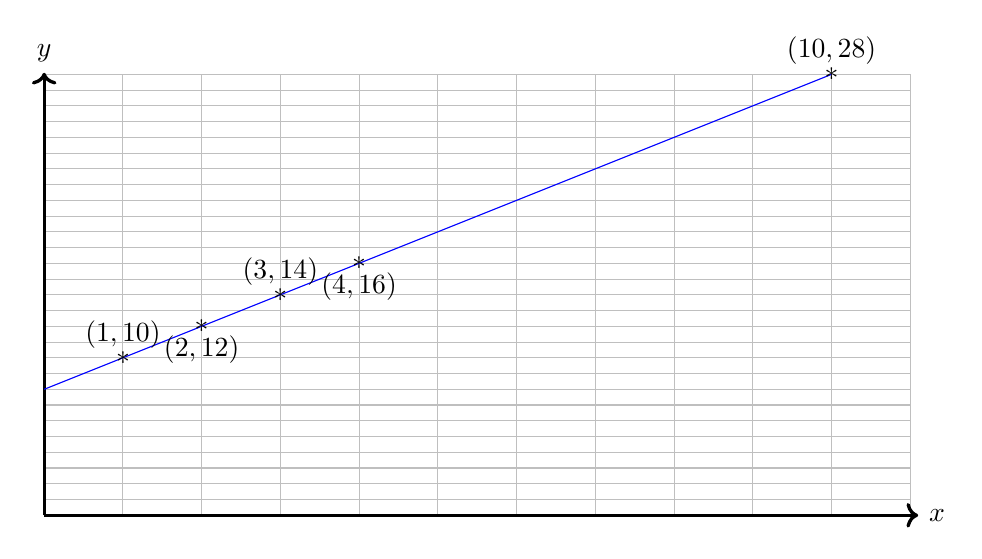
\begin{tikzpicture}[yscale=.2][domain=-0:11]
    \draw[gray!50, thin, step=1] (0,0) grid (11,28);
    \draw[very thick,->] (0,0) -- (11.1,0) node[right] {$x$};
    \draw[very thick,->] (0,0) -- (0,28.1) node[above] {$y$};

%    \foreach \x in {0,...,11} \draw (\x,0.05) -- (\x,-0.05) node[below] {\tiny\x};
%    \foreach \y in {0,...,28} \draw (-0.05,\y) -- (0.05,\y) node[right] {\tiny\y};


  \draw[scale=1,domain=0:10,smooth,variable=\x,blue] plot ({\x},{2*\x+8});

\node at (1,10){$*$};
\draw (1,10) --node[above]{$(1,10)$}(1,10);

\node at (2,12){$*$};
\draw (2,12) --node[below]{$(2,12)$}(2,12);

\node at (3,14){$*$};
\draw (3,14) --node[above]{$(3,14)$}(3,14);

\node at (4,16){$*$};
\draw (4,16) --node[below]{$(4,16)$}(4,16);

\node at (10,28){$*$};
\draw (10,28) --node[above]{$(10,28)$}(10,28);




\end{tikzpicture}$$ % of mbox

An interactive version of this graph may be found here: \url{https://www.desmos.com/calculator/9hocfhhs1m}.


\end{example}


It always helps to illustrate a concept with a \textbf{non}-example.

\begin{example}
Consider a function who takes on the following values:

$$\begin{array}{|c||c|c|c|c|c|}
\hline
x & -2&-1&0&1&2\\
\hline
f(x)&4&1&0&1&4\\
\hline
\end{array}
$$

\textbf{Question:} Does this function appear linear?\\

\textbf{Solution:}If we observe the change from $x=-2$ to $x=-1$, the change in $f(x)$ or $\Delta f(x)=1-4=-3$. 

 However, when we go from $x=-1$ to $x=0$, we see that $\Delta f(x)=0-1=-1$.  Similarly,   when we go from $x=0$ to $x=1$, we see that $\Delta f(x)=1-0=1$, and when we go from $x=1$ to $x=2$, we see that $\Delta f(x)=4-1=3$.
 
 Thus, this function goes from decreasing, to increasing, and the rate at which it does so changes, thus this function is \textbf{not} a linear function.


Graphically we can visualize this:

$$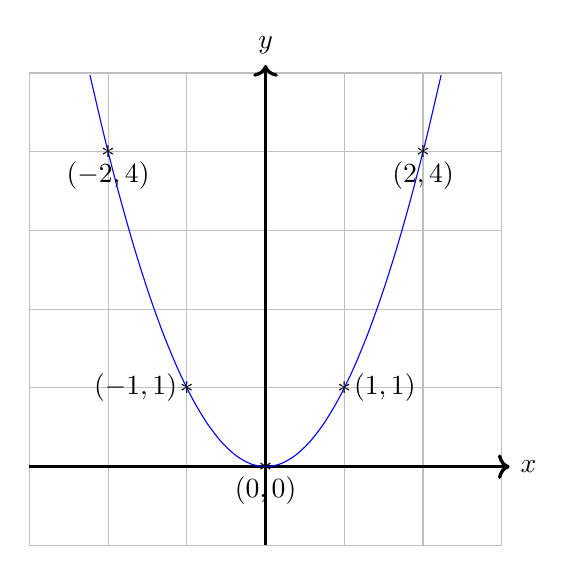
\begin{tikzpicture}[scale=1][domain=-0:11]
    \draw[gray!50, thin, step=1] (-3,-1) grid (3,5);
    \draw[very thick,->] (-3,0) -- (3.1,0) node[right] {$x$};
    \draw[very thick,->] (0,-1) -- (0,5.1) node[above] {$y$};

%    \foreach \x in {0,...,11} \draw (\x,0.05) -- (\x,-0.05) node[below] {\tiny\x};
%    \foreach \y in {0,...,28} \draw (-0.05,\y) -- (0.05,\y) node[right] {\tiny\y};


  \draw[scale=1,domain=-2.23:2.23,smooth,variable=\x,blue] plot ({\x},{\x*\x});

\node at (-2,4){$*$};
\draw (-2,4) --node[below]{$(-2,4)$}(-2,4);

\node at (-1,1){$*$};
\draw (-1,1) --node[left]{$(-1,1)$}(-1,1);

\node at (0,0){$*$};
\draw (0,0) --node[below]{$(0,0)$}(0,0);

\node at (1,1){$*$};
\draw (1,1) --node[right]{$(1,1)$}(1,1);

\node at (2,4){$*$};
\draw (2,4) --node[below]{$(2,4)$}(2,4);




\end{tikzpicture}$$ % of mbox

An interactive version of this graph may be found here: \url{https://www.desmos.com/calculator/za4t3zanlr}.


\end{example}


We can see from the above examples that linear functions are the functions whose graphs may be represented with a straight line.  This is sensible: after all, straight lines move in the same direction, and neither deviate one way nor another, just as linear functions increase, stay constant or decrease at a constant rate.  This is where the name \textbf{linear} functions come from.\\


\section{Standard form and graphs of Linear Functions.}\label{Section:GraphsofLinearFunctions}

Algebraically, linear functions are expressible as:

\begin{eqnarray*}
y&=&mx+b, \text{or}\\
f(x)&=&mx+b.
\end{eqnarray*}
%
Where $m$ is the \textbf{slope}, the rate of change of our linear function, and $b$ is the $\mathbf{y}$\textbf{-intercept}.\\



\textbf{Question:} What are these things, why do they have these names, and what do they signify?\\


\subsection{Slope.}


The \textbf{slope} is the constant rate of change of the linear function.  It is often expressed: $$m=\frac{\Delta y}{\Delta x}, m=\frac{\Delta f(x)}{\Delta x}.$$

These algebraic expressions are just a formal way of saying, ``However much $x$ changes, $y$ or $f(x)$ always changes by a proportional amount, and this amount is $m$."


\begin{example}\label{Example:Slope}
Let $y=-x+4$.  This represents a linear function with $m=-1$ and $b=4$.  To verify, if we compared $x=4$ and $x=1$, we have a change in $x$, $\Delta x=4-1=3$.  To find $\Delta y$, we note that when $x=1, y=-(1)+4=3$ and when $x=4, y=-(4)+4=0$.  Thus $\Delta y=0-3=-3$.  So $m=\frac{\Delta f(x)}{\Delta x}=\frac{-3}{3}=-1$.

This shouldn't depend on which choices of $x$ we made.  If we compared $x=3$ and $x=2$, we have a change in $x$, $\Delta x=3-2=1$.  To find $\Delta y$, we note that when $x=3, y=-(3)+4=1$ and when $x=2, y=-(2)+4=2$.  Thus $\Delta y=1-2=-1$.  So $m=\frac{\Delta f(x)}{\Delta x}=\frac{-1}{1}=-1$.

This can be represented visually:

$$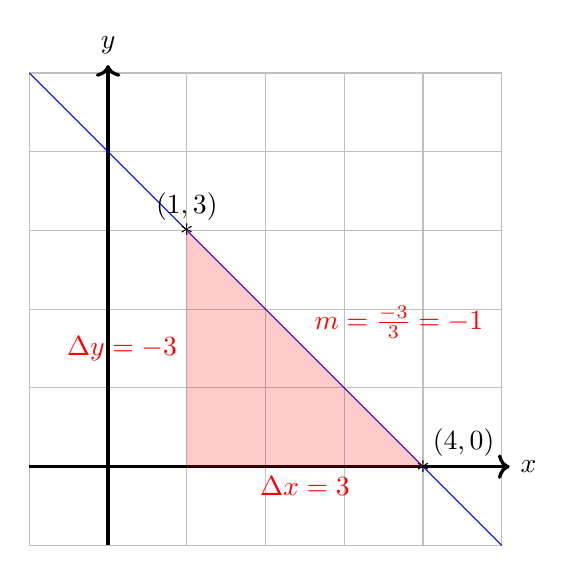
\begin{tikzpicture}[scale=1][domain=-1:5]
    \draw[gray!50, thin, step=1] (-1,-1) grid (5,5);
    \draw[very thick,->] (-1,0) -- (5.1,0) node[right] {$x$};
    \draw[very thick,->] (0,-1) -- (0,5.1) node[above] {$y$};

%    \foreach \x in {0,...,11} \draw (\x,0.05) -- (\x,-0.05) node[below] {\tiny\x};
%    \foreach \y in {0,...,28} \draw (-0.05,\y) -- (0.05,\y) node[right] {\tiny\y};


  \draw[scale=1,domain=-1:5,smooth,variable=\x,blue] plot ({\x},{-1*\x+4});

\node at (1,3){$*$};
\draw (1,3) --node[above]{$(1,3)$}(1,3);

\node at (4,0){$*$};
\draw (4,0) --node[above right]{$(4,0)$}(4,0);

\draw[red, fill, opacity=0.2] (1,3)--(4,0)--(1,0)--(1,3);

\draw[red] (1,1.5) --node[left]{$\Delta y =-3$}(1,1.5);

\draw[red] (2.5,0) --node[below]{$\Delta x =3$}(2.5,0);

\draw[red] (2.5,1.5) --node[above right]{$m=\frac{-3}{3}=-1$}(2.5,1.5);




\end{tikzpicture}%
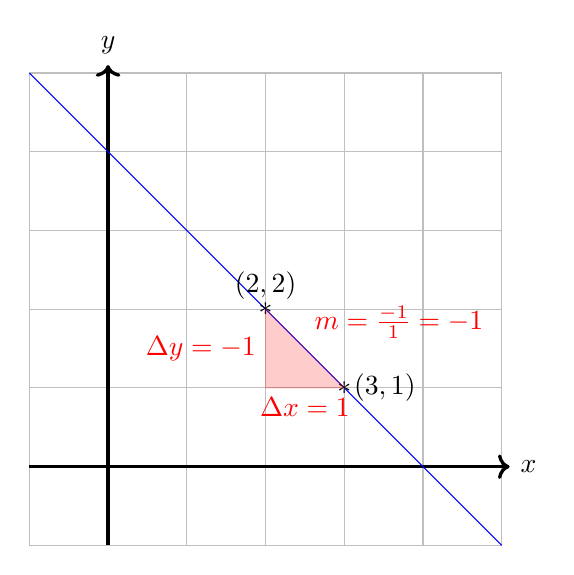
\begin{tikzpicture}[scale=1][domain=-1:5]
    \draw[gray!50, thin, step=1] (-1,-1) grid (5,5);
    \draw[very thick,->] (-1,0) -- (5.1,0) node[right] {$x$};
    \draw[very thick,->] (0,-1) -- (0,5.1) node[above] {$y$};

%    \foreach \x in {0,...,11} \draw (\x,0.05) -- (\x,-0.05) node[below] {\tiny\x};
%    \foreach \y in {0,...,28} \draw (-0.05,\y) -- (0.05,\y) node[right] {\tiny\y};


  \draw[scale=1,domain=-1:5,smooth,variable=\x,blue] plot ({\x},{-1*\x+4});

\node at (2,2){$*$};
\draw (2,2) --node[above]{$(2,2)$}(2,2);

\node at (3,1){$*$};
\draw (3,1) --node[right]{$(3,1)$}(3,1);

\draw[red, fill, opacity=0.2] (2,2)--(3,1)--(2,1)--(2,2);

\draw[red] (2,1.5) --node[left]{$\Delta y =-1$}(2,1.5);

\draw[red] (2.5,1) --node[below]{$\Delta x =1$}(2.5,1);

\draw[red] (2.5,1.5) --node[above right]{$m=\frac{-1}{1}=-1$}(2.5,1.5);




\end{tikzpicture}$$ % of mbox


An interactive version of this graph can be found here:  \url{https://www.desmos.com/calculator/9s3kfotxne}.



\end{example}

\begin{example}\label{Example:NullSlope}
Let $y=3$.  We can re-imagine this as $y=0x+3$, so this represents a linear function with $m=0$ and $b=3$.  Note that no matter what the $x$ values are, $y=3$.  So $\Delta y=0$, and $m=\frac{\Delta y}{\Delta x}=\frac{0}{\Delta x}=0$.  Intuitively, $y$ is always 3 and never changes, so the ``rate of change" is a constant nothing.  This gives us a horizontal line.

This can be represented visually:

$$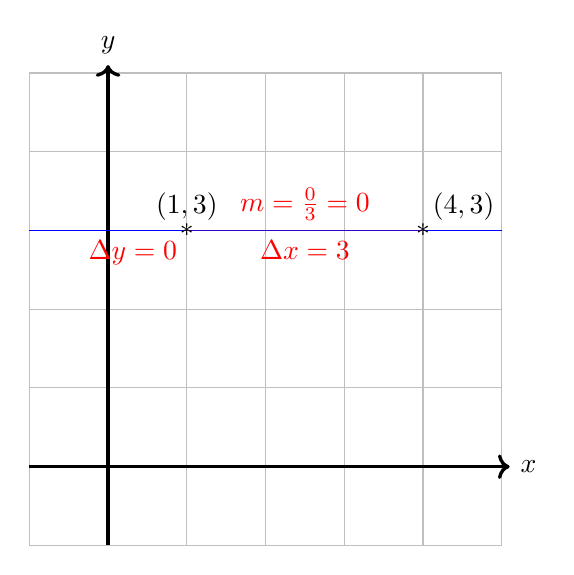
\begin{tikzpicture}[scale=1][domain=-1:5]
    \draw[gray!50, thin, step=1] (-1,-1) grid (5,5);
    \draw[very thick,->] (-1,0) -- (5.1,0) node[right] {$x$};
    \draw[very thick,->] (0,-1) -- (0,5.1) node[above] {$y$};


  \draw[scale=1,domain=-1:5,smooth,variable=\x,blue] plot ({\x},{3});

\node at (1,3){$*$};
\draw (1,3) --node[above]{$(1,3)$}(1,3);

\node at (4,3){$*$};
\draw (4,3) --node[above right]{$(4,3)$}(4,3);

\draw[red, opacity=0.2] (1,3)--(4,3);

\draw[red] (1,3) --node[below left]{$\Delta y =0$}(1,3);

\draw[red] (2.5,3) --node[below]{$\Delta x =3$}(2.5,3);

\draw[red] (2.5,3) --node[above]{$m=\frac{0}{3}=0$}(2.5,3);



\end{tikzpicture}%
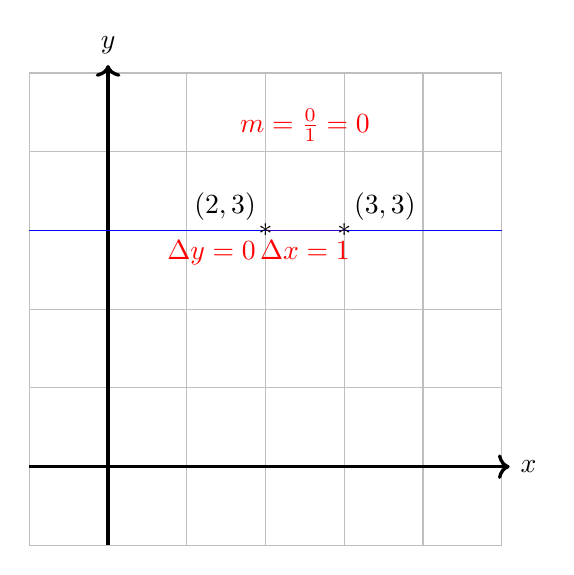
\begin{tikzpicture}[scale=1][domain=-1:5]
    \draw[gray!50, thin, step=1] (-1,-1) grid (5,5);
    \draw[very thick,->] (-1,0) -- (5.1,0) node[right] {$x$};
    \draw[very thick,->] (0,-1) -- (0,5.1) node[above] {$y$};


  \draw[scale=1,domain=-1:5,smooth,variable=\x,blue] plot ({\x},{3});

\node at (2,3){$*$};
\draw (2,3) --node[above left]{$(2,3)$}(2,3);

\node at (3,3){$*$};
\draw (3,3) --node[above right]{$(3,3)$}(3,3);

\draw[red, opacity=0.2] (2,3)--(3,3);

\draw[red] (2,3) --node[below left]{$\Delta y =0$}(2,3);

\draw[red] (2.5,3) --node[below]{$\Delta x =1$}(2.5,3);

\draw[red] (2.5,4) --node[above]{$m=\frac{0}{1}=0$}(2.5,4);




\end{tikzpicture}%
$$ % of mbox


An interactive version of this graph can be found here:  \url{https://www.desmos.com/calculator/pv7m6fbugb}.



\end{example}

\subsection{$\mathbf{y}$-intercept.}

The $\mathbf{y}$\textbf{-intercept} of a linear function $y=mx+b$ is the value $b$.  It is so named because it is the value of the linear function when it \textbf{intercepts} the $y$-axis.  The reason for this is that the $y$-axis is exactly the line $x=0$, and when $x=0$, $y=m(0)+b=b$.


\begin{example}\label{Example:Intercept}
Let us recall Example \ref{Example:Slope} and let $y=-x+4$.  Note that when $x=0, y=-(0)+4=4$.

This can be represented visually:

$$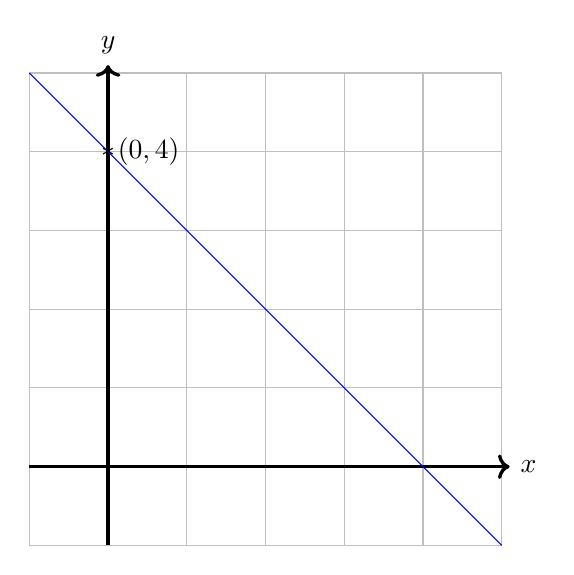
\begin{tikzpicture}[scale=1][domain=-1:5]
    \draw[gray!50, thin, step=1] (-1,-1) grid (5,5);
    \draw[very thick,->] (-1,0) -- (5.1,0) node[right] {$x$};
    \draw[very thick,->] (0,-1) -- (0,5.1) node[above] {$y$};

%    \foreach \x in {0,...,11} \draw (\x,0.05) -- (\x,-0.05) node[below] {\tiny\x};
%    \foreach \y in {0,...,28} \draw (-0.05,\y) -- (0.05,\y) node[right] {\tiny\y};


  \draw[scale=1,domain=-1:5,smooth,variable=\x,blue] plot ({\x},{-1*\x+4});

\node at (0,4){$*$};
\draw (0,4) --node[right]{$(0,4)$}(0,4);





\end{tikzpicture}$$ % of mbox


Note that $4$ is the height of the function when it intercepts the $y$-axis.


\end{example}

\begin{example}\label{Example:Intercept2}
Let us recall Example \ref{Example:NullSlope} and let $y=3=0x+3$.  Note that when $x=0, y=3$.

This can be represented visually:

$$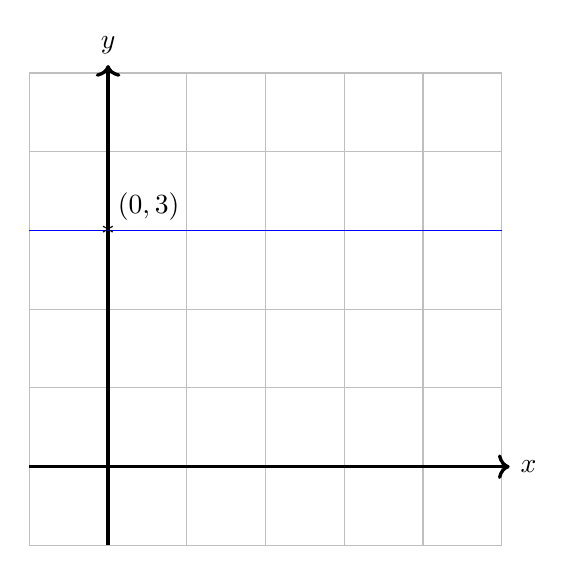
\begin{tikzpicture}[scale=1][domain=-1:5]
    \draw[gray!50, thin, step=1] (-1,-1) grid (5,5);
    \draw[very thick,->] (-1,0) -- (5.1,0) node[right] {$x$};
    \draw[very thick,->] (0,-1) -- (0,5.1) node[above] {$y$};

%    \foreach \x in {0,...,11} \draw (\x,0.05) -- (\x,-0.05) node[below] {\tiny\x};
%    \foreach \y in {0,...,28} \draw (-0.05,\y) -- (0.05,\y) node[right] {\tiny\y};


  \draw[scale=1,domain=-1:5,smooth,variable=\x,blue] plot ({\x},{3});

\node at (0,3){$*$};
\draw (0,3) --node[above right]{$(0,3)$}(0,3);





\end{tikzpicture}$$ % of mbox


Note that $3$ is the height of the function when it intercepts the $y$-axis.


\end{example}


\subsection{Translating from Algebra to Geometry}

We can see in our above examples that linear functions have both an algebraic form and a geometric interpretation.   Both are useful and in fact necessary to understand what's going on with a linear function.  So what we now want to ask ourselves is, given the algebraic expression for a line, how might we find it's geometric representation?\\


Intuitively, we know that if we had a sheet of paper and a ruler, if we drew 2 points on this paper, we could find the line between them.  So to find a geometric representation of a linear function, we should:

\begin{enumerate}
    \item Find a point that must be on thee line.
    \item Identify a second point on the line.
    \item Draw the line between them.
\end{enumerate}

\begin{example}\label{Example:DrawLine}
\textbf{Question:} Draw the line $y=f(x)$ where $f(x)=-\frac{2}{3}x+4$.

\begin{enumerate}
    \item We first identify a point on the line, the easiest to find is probably the $y$-intercept, note that when $x=0, f(x)=-\frac{2}{3}(0)+4=4$, thus $(0,4)$ is on $y=f(x)$.
    \item We have infinitely many choices for a second point, but to make the arithmetic easy, let's let $x=3$, then $f(x)=-\frac{2}{3}(3)+4=-2+4=2$, so $(3,2)$ is on the line.
    
    Note this gives us:
 $$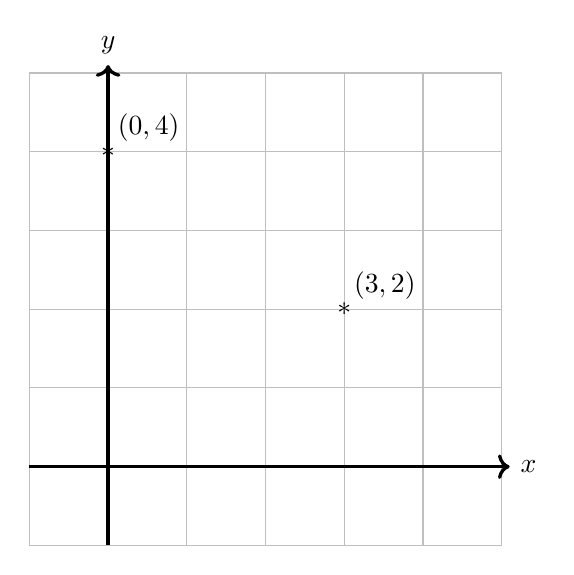
\begin{tikzpicture}[scale=1][domain=-1:5]
    \draw[gray!50, thin, step=1] (-1,-1) grid (5,5);
    \draw[very thick,->] (-1,0) -- (5.1,0) node[right] {$x$};
    \draw[very thick,->] (0,-1) -- (0,5.1) node[above] {$y$};

%    \foreach \x in {0,...,11} \draw (\x,0.05) -- (\x,-0.05) node[below] {\tiny\x};
%    \foreach \y in {0,...,28} \draw (-0.05,\y) -- (0.05,\y) node[right] {\tiny\y};


%  \draw[scale=1,domain=-1:5,smooth,variable=\x,blue] plot ({\x},{(-2/3)*\x+4});

\node at (0,4){$*$};
\draw (0,4) --node[above right]{$(0,4)$}(0,4);

\node at (3,2){$*$};
\draw (3,2) --node[above right]{$(3,2)$}(3,2);




\end{tikzpicture}$$    
    \item We then literally connect the dots:
$$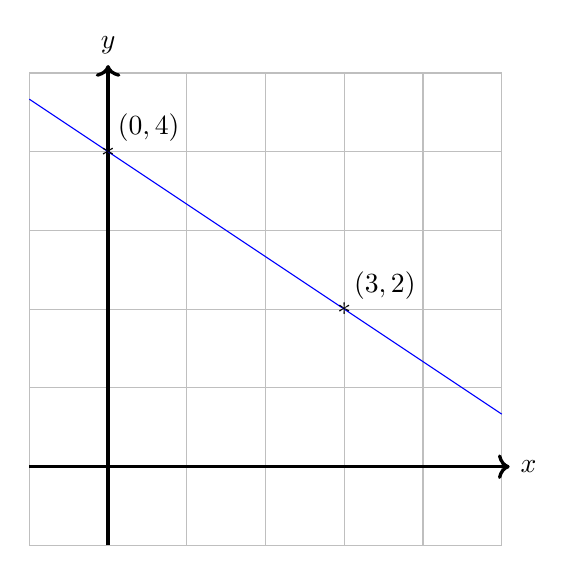
\begin{tikzpicture}[scale=1][domain=-1:5]
    \draw[gray!50, thin, step=1] (-1,-1) grid (5,5);
    \draw[very thick,->] (-1,0) -- (5.1,0) node[right] {$x$};
    \draw[very thick,->] (0,-1) -- (0,5.1) node[above] {$y$};

%    \foreach \x in {0,...,11} \draw (\x,0.05) -- (\x,-0.05) node[below] {\tiny\x};
%    \foreach \y in {0,...,28} \draw (-0.05,\y) -- (0.05,\y) node[right] {\tiny\y};


  \draw[scale=1,domain=-1:5,smooth,variable=\x,blue] plot ({\x},{(-2/3)*\x+4});

\node at (0,4){$*$};
\draw (0,4) --node[above right]{$(0,4)$}(0,4);

\node at (3,2){$*$};
\draw (3,2) --node[above right]{$(3,2)$}(3,2);




\end{tikzpicture}$$      
\end{enumerate}
Modern technology also let's us readily draw these functions: \url{https://www.desmos.com/calculator/gyvulordwz}.
\end{example}

\begin{example}\label{Example:DrawLineOtherForm}
\textbf{Question:} Draw the line $2x+4y=8$.

\begin{enumerate}
    \item We first identify a point on the line.  To make life easy note that when $x=0, 2(0)+4y=8$ and $y=2$, thus $(0,2)$ is on $2x+4y=8$.
    \item Similarly when $y=0, 2x+4(0)=8$ and $x=4$, thus $(4,0)$ is on $2x+4y=8$.
    
    Note this gives us:
 $$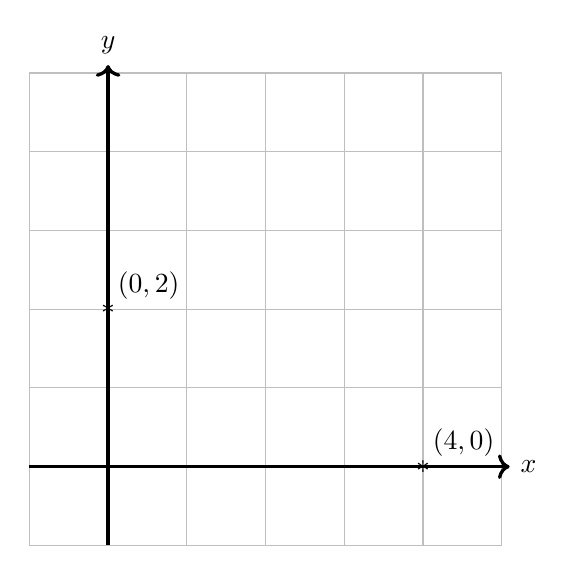
\begin{tikzpicture}[scale=1][domain=-1:5]
    \draw[gray!50, thin, step=1] (-1,-1) grid (5,5);
    \draw[very thick,->] (-1,0) -- (5.1,0) node[right] {$x$};
    \draw[very thick,->] (0,-1) -- (0,5.1) node[above] {$y$};

%    \foreach \x in {0,...,11} \draw (\x,0.05) -- (\x,-0.05) node[below] {\tiny\x};
%    \foreach \y in {0,...,28} \draw (-0.05,\y) -- (0.05,\y) node[right] {\tiny\y};


%  \draw[scale=1,domain=-1:5,smooth,variable=\x,blue] plot ({\x},{(-1/2)*\x+2});

\node at (0,2){$*$};
\draw (0,2) --node[above right]{$(0,2)$}(0,2);

\node at (4,0){$*$};
\draw (4,0) --node[above right]{$(4,0)$}(4,0);




\end{tikzpicture}$$    
    \item We then connect the dots:
$$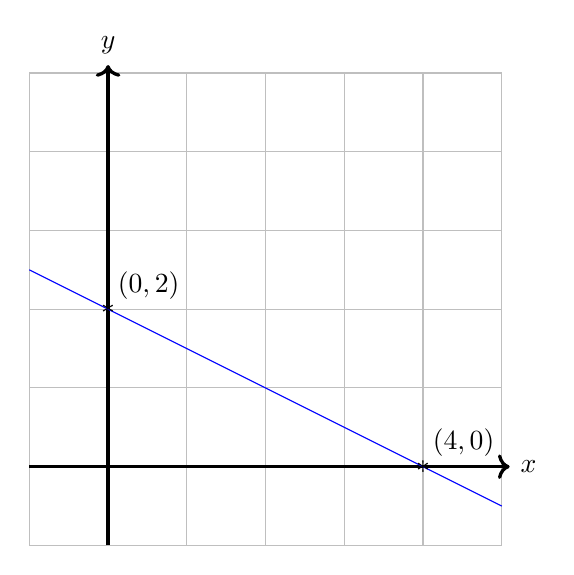
\begin{tikzpicture}[scale=1][domain=-1:5]
    \draw[gray!50, thin, step=1] (-1,-1) grid (5,5);
    \draw[very thick,->] (-1,0) -- (5.1,0) node[right] {$x$};
    \draw[very thick,->] (0,-1) -- (0,5.1) node[above] {$y$};

%    \foreach \x in {0,...,11} \draw (\x,0.05) -- (\x,-0.05) node[below] {\tiny\x};
%    \foreach \y in {0,...,28} \draw (-0.05,\y) -- (0.05,\y) node[right] {\tiny\y};


  \draw[scale=1,domain=-1:5,smooth,variable=\x,blue] plot ({\x},{(-1/2)*\x+2});

\node at (0,2){$*$};
\draw (0,2) --node[above right]{$(0,2)$}(0,2);

\node at (4,0){$*$};
\draw (4,0) --node[above right]{$(4,0)$}(4,0);




\end{tikzpicture}$$          
\end{enumerate}
Again, utilizing technology: \url{https://www.desmos.com/calculator/lprlevpf6q}.\\

Note that we could have taken $2x+4y=8$ and rewritten it:

\begin{eqnarray*}
2x+4y&=&8\\
4y&=&-2x+8\\
y&=&-\frac{1}{2}x+2,
\end{eqnarray*}

and from here, treated it the same way as in Example \ref{Example:DrawLine}.

\end{example}



\section{Identifying a Linear Function from information.}\label{Section:IndentifyLinear}


It is often the case that when one works with a linear function, one will not be given the exact form for the function.  You may for example only know the rate of change, or the value of the function at a few points.  To be able to make the most of this situation, it would be good to be able to still identify the linear function in question, when possible.\\

\textbf{Question:}  What is the minimal amount of information necessary to identify a linear function?\\

Here is where our geometric interpretation of these functions is helpful.  If someone handed you a sheet of paper and asked you to draw a line, how much information would they have to give you so there could be only one like you'd be able to draw?\\

\textbf{Question:}  Is a point enough?\\

If someone drew a dot on a piece of paper, there is certainly a line you could draw through it, but it definitely does seem like there's infinitely many lines you could draw as well.  Take $(2,3)$:

$$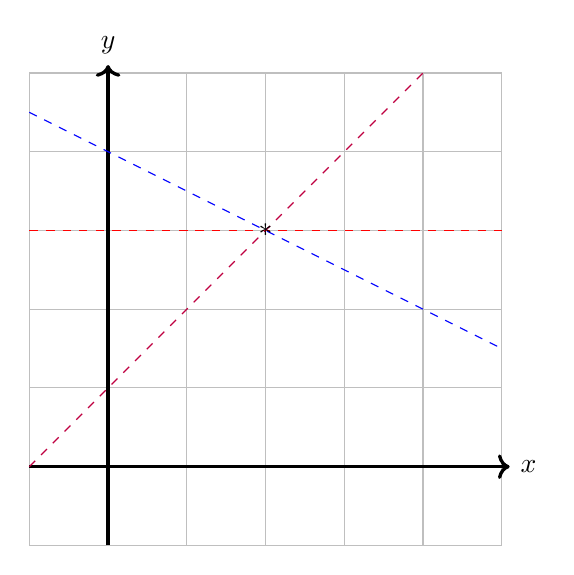
\begin{tikzpicture}[scale=1][domain=-1:5]
    \draw[gray!50, thin, step=1] (-1,-1) grid (5,5);
    \draw[very thick,->] (-1,0) -- (5.1,0) node[right] {$x$};
    \draw[very thick,->] (0,-1) -- (0,5.1) node[above] {$y$};

%    \foreach \x in {0,...,11} \draw (\x,0.05) -- (\x,-0.05) node[below] {\tiny\x};
%    \foreach \y in {0,...,28} \draw (-0.05,\y) -- (0.05,\y) node[right] {\tiny\y};


    \draw[scale=1,domain=-1:5,smooth,variable=\x,blue, dashed] plot ({\x},{(-1/2)*\x+4});
  
    \draw[scale=1,domain=-1:5,smooth,variable=\x,red, dashed] plot ({\x},{3});
    
    \draw[scale=1,domain=-1:4,smooth,variable=\x,purple, dashed] plot ({\x},{\x+1});

\node at (2,3){$*$};

\end{tikzpicture}$$   

Of course there are many more, here's a visualization: \url{https://www.desmos.com/calculator/c3gronrfd3}.



\textbf{Question:}  Is a slope/direction enough?\\

If someone gave you a piece of paper and told you would direction the line should take, there is definitely a line you could draw with that direction, but depending where you start, there's infinitely many lines you could draw as well.  Take $m=\frac{3}{2}$:

$$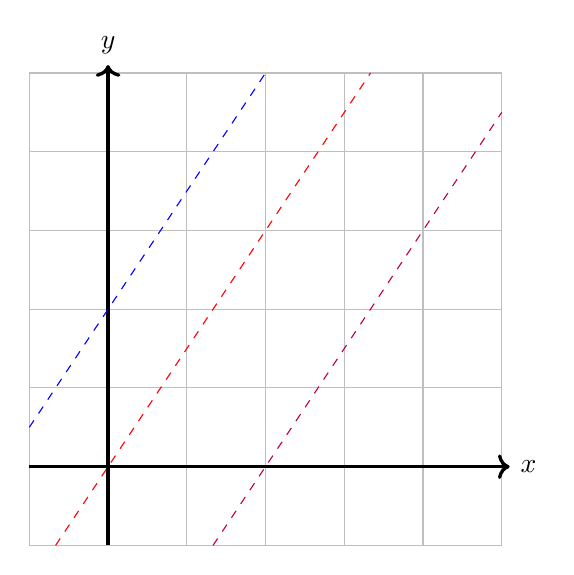
\begin{tikzpicture}[scale=1][domain=-1:5]
    \draw[gray!50, thin, step=1] (-1,-1) grid (5,5);
    \draw[very thick,->] (-1,0) -- (5.1,0) node[right] {$x$};
    \draw[very thick,->] (0,-1) -- (0,5.1) node[above] {$y$};

%    \foreach \x in {0,...,11} \draw (\x,0.05) -- (\x,-0.05) node[below] {\tiny\x};
%    \foreach \y in {0,...,28} \draw (-0.05,\y) -- (0.05,\y) node[right] {\tiny\y};


    \draw[scale=1,domain=-1:2,smooth,variable=\x,blue, dashed] plot ({\x},{(3/2)*\x+2});
  
    \draw[scale=1,domain=-2/3:10/3,smooth,variable=\x,red, dashed] plot ({\x},{(3/2)*\x});
    
    \draw[scale=1,domain=4/3:5,smooth,variable=\x,purple, dashed] plot ({\x},{(3/2)*\x-3});


\end{tikzpicture}$$   

Of course there are many more, here's a visualization: \url{https://www.desmos.com/calculator/iwcjwhen1b}.


So this begs the question, what \textbf{IS} the mininum amount of information that you'd need to uniquely identify a line?

\subsection{Point \& Slope}

If we combined the two pieces of information from the start of the section, would we obtain a unique line?  Intuitively this should make sense, there are infinitely many lines which go through a point, but only one with slope $m=\frac{3}{2}$, similarly, there are infinitely many lines with slope $\frac{3}{2}$, but they all pass through different points, only one of them passes through $(2,3)$.  Again to refer to our geometric ideas, if someone drew a point on a paper, and told you which direction you had to go from there, there's really only one line you could draw.\\

Here are some visualizations:  

$$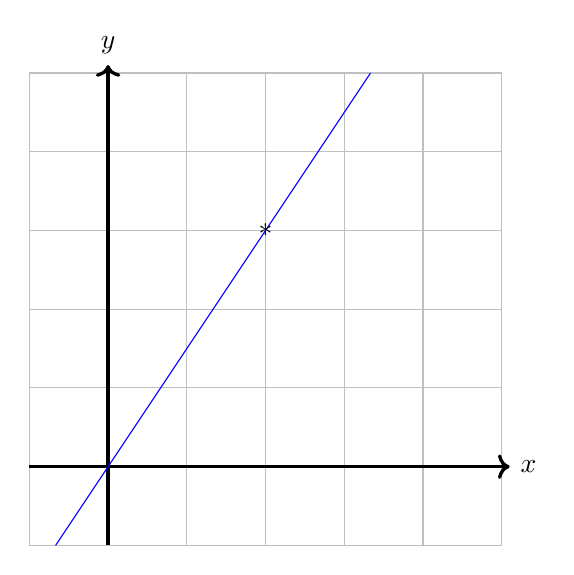
\begin{tikzpicture}[scale=1][domain=-1:5]
    \draw[gray!50, thin, step=1] (-1,-1) grid (5,5);
    \draw[very thick,->] (-1,0) -- (5.1,0) node[right] {$x$};
    \draw[very thick,->] (0,-1) -- (0,5.1) node[above] {$y$};



%    \foreach \x in {0,...,11} \draw (\x,0.05) -- (\x,-0.05) node[below] {\tiny\x};
%    \foreach \y in {0,...,28} \draw (-0.05,\y) -- (0.05,\y) node[right] {\tiny\y};


    \draw[scale=1,domain=-2/3:10/3,smooth,variable=\x,blue] plot ({\x},{(3/2)*\x});
  

\node at (2,3){$*$};

\end{tikzpicture}$$   



\url{https://www.desmos.com/calculator/5ikul0ktn5}, \url{https://www.desmos.com/calculator/hcl8ynd0yp}.

\textbf{Question:} How does this translate Algebraically?

So given a linear function is defined by the slope $m$ and intercept $b$.  By the discussion above, if we are given a slope $\textcolor{red}{m}$ and a pair of points $\textcolor{blue}{(x_0,y_0)}$, we should be able to uniquely identify $b$.

\begin{example}\label{Example:PandS}
\textbf{Question:}  Find the linear function with slope 3 passing through $(2,5)$.\\

Note that we are given $\textcolor{red}{m=3}$ and $\textcolor{blue}{(x_0,y_0)=(2,5)}$.  The general form for a line is $y=mx+b$, thus:

\begin{eqnarray*}
y&=&mx+b\\
\textcolor{blue}{5}&=&\textcolor{red}{3}\cdot\textcolor{blue}{2}+b\\
5&=&6+b\\
b&=&5-6=-1.\\
\end{eqnarray*}

Thus $y=3x-1$ is the linear equation in question, $m=3, b=-1$.

$$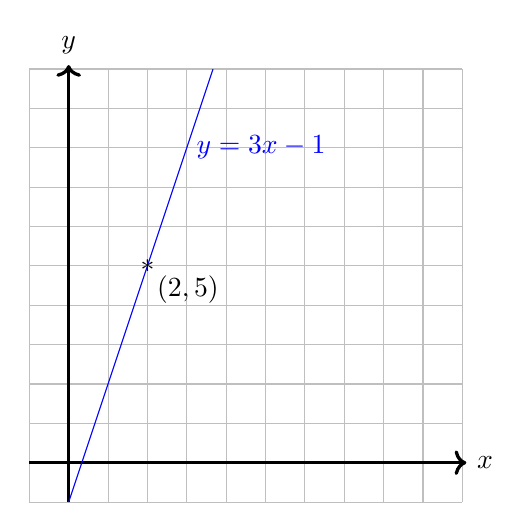
\begin{tikzpicture}[scale=0.5][domain=-1:10]
    \draw[gray!50, thin, step=1] (-1,-1) grid (10,10);
    \draw[very thick,->] (-1,0) -- (10.1,0) node[right] {$x$};
    \draw[very thick,->] (0,-1) -- (0,10.1) node[above] {$y$};

%    \foreach \x in {0,...,11} \draw (\x,0.05) -- (\x,-0.05) node[below] {\tiny\x};
%    \foreach \y in {0,...,28} \draw (-0.05,\y) -- (0.05,\y) node[right] {\tiny\y};


    \draw[scale=1,domain=0:3.666,smooth,variable=\x,blue] plot ({\x},{(3)*\x-1});
  

\node at (2,5){$*$};
\draw (2,5) --node[below right]{$(2,5)$}(2,5);
\draw[blue] (3,8) --node[right]{$y=3x-1$}(3,8);



\end{tikzpicture}$$   
\url{https://www.desmos.com/calculator/w3nixbtfrs}.

We can verify that this line has slope $m=3$ and when $x=2, y=3\cdot 2-1=6-1=5$.

\end{example}


\subsection{Point-Slope form.}

So, typically lines are defined in the form $y=mx+b$, where $m$ is the slope and $b$ is the $y$-intercept.  It can be convenient to also define a line in the form $$y-y_0=m(x-x_0),$$ where $(x_0, y_0)$ is a point that falls on your line.\\

Why would we care about a second formulation, and how do we know it's even a line?  To answer the first question, we recall that ANY geometric object defined by an equation is the set of points that make the equation true.  So given the equation $y-y_0=m(x-x_0)$, if we plug in $(x_0, y_0)$, we would get $y_0-y_0=m(x_0-x_0)$ or $0=0$ which is definitely a true statement.  So whatever shape we get from $y-y_0=m(x-x_0)$, it contains $(x_0, y_0)$.\\

We know it's a line because:

\begin{eqnarray*}
y-y_0&=&m(x-x_0)\\
y&=&mx-mx_0+y_0\\
y&=&mx+(y_0-mx_0)
\end{eqnarray*}

so if we let $b=y_0-mx_0$, we get the standard form for a line.


\begin{example}\label{Example:PandSagain}
\textbf{Question:} Find the line with slope 3 passing through $(2,5)$, again.\\

Using the point-slope form, knowing that $\textcolor{blue}{(2,5)}$ lies on the line, and that $\textcolor{red}{m}$:

\begin{eqnarray*}
y-y_0&=&m(x-x_0)\\
y-\textcolor{blue}{5}&=&\textcolor{red}{3}(x-\textcolor{blue}{2})\\
y&=&3x-6+5\\
y&=&3x-1.
\end{eqnarray*}

Either way, you obtain the same line, with slope 3, passing through (2,5).

\end{example}

\subsection{Two Points}

On the other hand, instead of giving you a point and a direction, one could be given two points to traverse through.  If you imagine any two dots on a piece of paper, one can imagine that you may draw a line between them.  The exact way we do this also follows intuitively.  If you were at home, and you had to go to the store, the natural steps you would take to do so are:

\begin{enumerate}
\item Figure out which way to the store.
\item Go there.
\end{enumerate}

So we have to figure out the direction between these points, which in our analogy means the slope between the points.  Remember the slope measures how much $y$ changes per change in $x$, or $m=\frac{\Delta y}{\Delta x}$.  So, the measurement of slope follows from the change in $y$ over the change in $x$.  So to measure this, if we have points $(x_0, y_0), (x_1, y_1)$, we want to see how much $y$ changes over how much $x$ changes, or:

$$m=\frac{\Delta y}{\Delta x}=\frac{y_1-y_0}{x_1-x_0}$$
or equivalently $m=\frac{y_0-y_1}{x_0-x_1}$.


\begin{example}\label{Example:PandP}
What line passes between $(2,3)$ and $(4,1)$?\\

So we note then that $\textcolor{red}{m=\frac{1-3}{4-2}=-1}$ (also $\textcolor{red}{m=\frac{3-1}{2-4}=-1}$).  Once the slope is identified, we can use any point, and any method to find the line.  Once we pick a point, We have a problem that follows the form of Examples \ref{Example:PandS}, \ref{Example:PandSagain}.

We won't go through all the possibilities but if we considered the point $\textcolor{blue}{(2,3)}$:

\begin{eqnarray*}
y&=&mx+b\\
\textcolor{blue}{3}&=&\textcolor{red}{-1}\cdot \textcolor{blue}{2}+b\\
b&=&3+2=5\\
y&=&-x+5.
\end{eqnarray*}

Or if we picked $\textcolor{blue}{(1,4)}$:

\begin{eqnarray*}
y-y_0&=&m(x-x_0)\\
y-\textcolor{blue}{1}&=&\textcolor{red}{-1}\cdot(x-\textcolor{blue}{4})\\
y&=&-x+4+1\\
y&=&-x+5.
\end{eqnarray*}

Either way, we identify the same line:

$$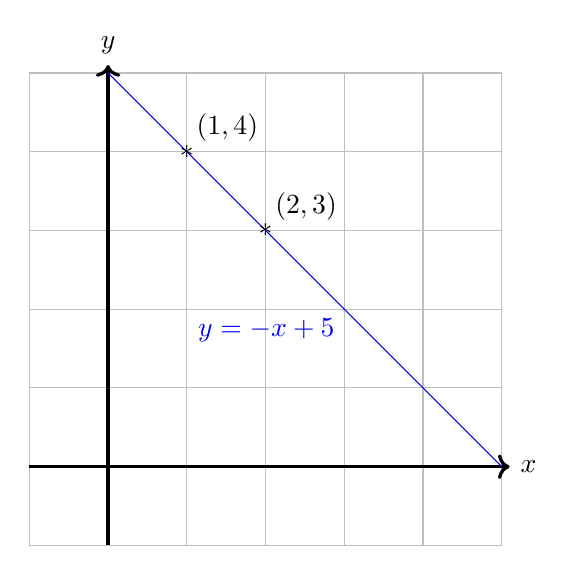
\begin{tikzpicture}[scale=1][domain=-1:5]
    \draw[gray!50, thin, step=1] (-1,-1) grid (5,5);
    \draw[very thick,->] (-1,0) -- (5.1,0) node[right] {$x$};
    \draw[very thick,->] (0,-1) -- (0,5.1) node[above] {$y$};

%    \foreach \x in {0,...,11} \draw (\x,0.05) -- (\x,-0.05) node[below] {\tiny\x};
%    \foreach \y in {0,...,28} \draw (-0.05,\y) -- (0.05,\y) node[right] {\tiny\y};


    \draw[scale=1,domain=0:5,smooth,variable=\x,blue] plot ({\x},{(-1)*\x+5});
  

\node at (2,3){$*$};
\draw (2,3) --node[above right]{$(2,3)$}(2,3);

\node at (1,4){$*$};
\draw (1,4) --node[above right]{$(1,4)$}(1,4);

\draw[blue] (3,2) --node[below left]{$y=-x+5$}(3,2);


\end{tikzpicture}$$  

\url{https://www.desmos.com/calculator/yohrdbuwuc}

\end{example}

\section{Utilizing the Linear Function}\label{Section:UtilityLinear}

Once you obtain a linear function, this gives you a relationship between the $x$ and $y$ variables.  It allows you to identify, given an $x$ or $y$ value, the other value:

\begin{example}\label{Example:LinearFindValue}
Consider the linear function $y=2x-3$.
\begin{enumerate}
\item When $y=0$, what is $x$?
\item When $x=3$ what is $y$?
\end{enumerate}

These can be identified algebraically:
\begin{enumerate}
\item When $\textcolor{ForestGreen}{y=0}$, we have:
\begin{eqnarray*}
y&=&2x-3\\
\textcolor{ForestGreen}{0}&=&2x-3\\
3&=&2x\\
x&=&1.5.
\end{eqnarray*}
\item If $\textcolor{orange}{x=3}$:
\begin{eqnarray*}
y&=&2x-3\\
y&=&2(\textcolor{orange}{3})-3\\
y&=&6-3=3.
\end{eqnarray*}
We can identify both points graphically as well:



\url{https://www.desmos.com/calculator/gukgr4sjfm}.
\end{enumerate}

$$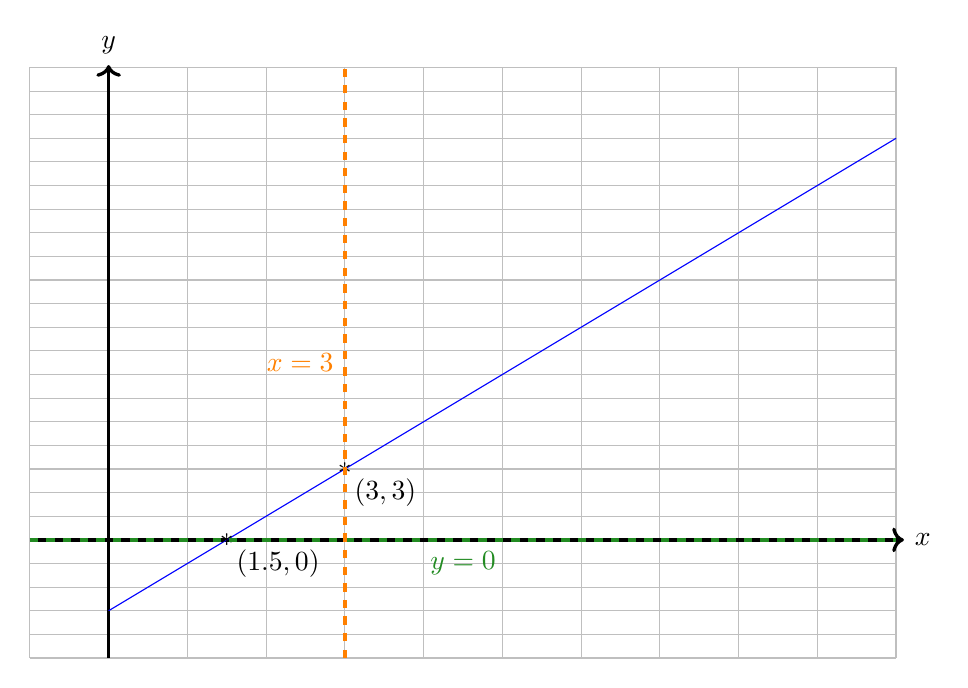
\begin{tikzpicture}[yscale=0.3][domain=-1:10]
    \draw[gray!50, thin, step=1] (-1,-5) grid (10,20);
    \draw[very thick,->] (-1,0) -- (10.1,0) node[right] {$x$};
    \draw[very thick,->] (0,-5) -- (0,20.1) node[above] {$y$};

%    \foreach \x in {0,...,11} \draw (\x,0.05) -- (\x,-0.05) node[below] {\tiny\x};
%    \foreach \y in {0,...,28} \draw (-0.05,\y) -- (0.05,\y) node[right] {\tiny\y};


    \draw[scale=1,domain=0:10,smooth,variable=\x,blue] plot ({\x},{(2)*\x-3});
  

\node at (1.5,0){$*$};
\draw (1.5,0) --node[below right]{$(1.5,0)$}(1.5,0);

\node at (3,3){$*$};
\draw (3,3) --node[below right]{$(3,3)$}(3,3);

\draw[ForestGreen, dashed, ultra thick] (-1,0) --node[below]{$y=0$}(10,0);

\draw[orange, dashed, ultra thick] (3,-5) --node[left]{$x=3$}(3,20);


\end{tikzpicture}$$  

\end{example}


\section{Applications of Linear Functions}\label{Section:ApplicationsLinear}

Up until this point, we've been treating linear functions as somewhat disembodied Mathematical entities.  In this section, we'll give a few examples to show how they appear and are applied in practice.


\begin{example}\label{Example:LinearTemp}

\Q The freezing point of water is $0^\circ$ Celsius and $32^\circ$ Fahrenheit.  The boiling point of water is $100^\circ$ Celsius and $212^\circ$ Fahrenheit.

\begin{enumerate}
    \item Find a linear function $T(F)=C$ that converts Fahrenheit into Celsius.
    \item When it's 10 degrees Fahrenheit, what is the temperature in Celsius?
    \item When it's 30 degrees Celsius, what is the temperature in Fahrenheit?
\end{enumerate}

\Sol We are given that $T(32)=0$ and $T(212)=100$.  This gives us points $(32,0)$ and $(212,100)$, so this bears some similarity to Example \ref{Example:PandP}.

\begin{enumerate}
    \item We first identify the slope of the function: $$m=\frac{\Delta C}{\Delta F}=\frac{100-0}{212-32}=\frac{100}{180}=\TCR{\frac{5}{9}}.$$
Then choosing either point, say $\TCB{(32,0)}$, and point slope form, we have:
\begin{eqnarray*}
C-C_0&=&m(F-F_0)\\
C-\TCB{0}&=&\TCR{\frac{5}{9}}(F-\TCB{32})\\
C&=&\frac{5}{9}F-\frac{160}{9}.
\end{eqnarray*}

Thus $T(F)=\frac{5}{9}F-\frac{160}{9}$

$$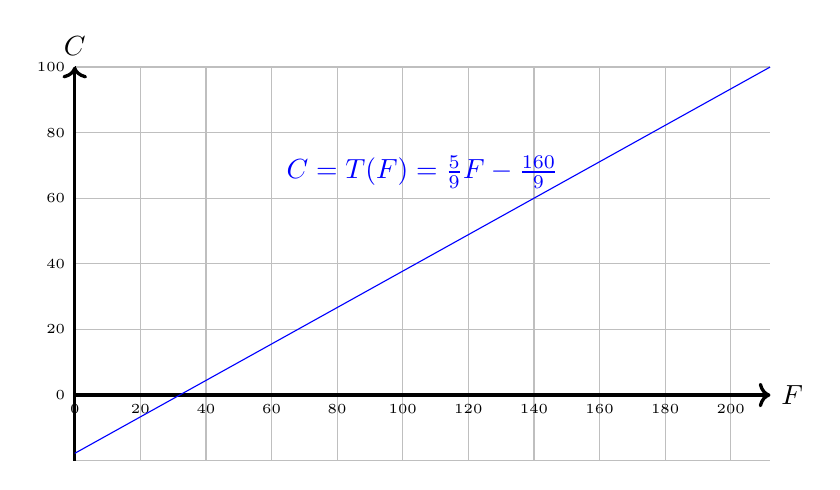
\begin{tikzpicture}[yscale=1/24, xscale=1/24][domain=-1:10]
    \draw[gray!50, thin, step=20] (0,-20) grid (212,100);
    \draw[very thick,->] (0,0) -- (212.1,0) node[right] {$F$};
    \draw[very thick,->] (0,-20) -- (0,100.1) node[above] {$C$};

    \foreach \x in {0,20,...,200} \draw (\x,0.05) -- (\x,-0.05) node[below] {\tiny\x};
    \foreach \y in {0,20,...,100} \draw (-0.05,\y) -- (0.05,\y) node[left] {\tiny\y};


    \draw[scale=1,domain=0:212,smooth,variable=\x,blue] plot ({\x},{(5/9)*\x-160/9});
  

\draw[blue] (106,60) --node[above]{$C=T(F)=\frac{5}{9}F-\frac{160}{9}$}(106,60);


\end{tikzpicture}$$ 

\item When it's 10 degrees, we have that $\TCG{F=10}$ and so:

\begin{eqnarray*}
C&=&\frac{5}{9}F-\frac{160}{9}\\
C&=&\frac{5}{9}\cdot\TCG{10}-\frac{160}{9}\\
C&=&\frac{50}{9}-\frac{160}{9}\\
C&=&-\frac{110}{9}\approx-12.2222.
\end{eqnarray*}
So 10 degrees Fahrenheit is $-\frac{110}{9}\approx-12.2222$ degrees Celsius.

$$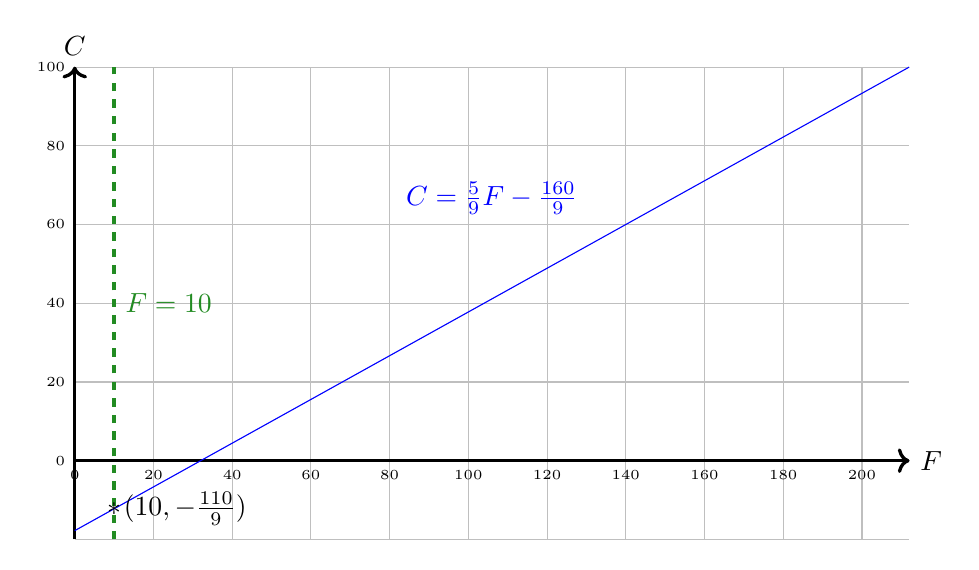
\begin{tikzpicture}[yscale=1/20, xscale=1/20][domain=-1:10]
    \draw[gray!50, thin, step=20] (0,-20) grid (212,100);
    \draw[very thick,->] (0,0) -- (212.1,0) node[right] {$F$};
    \draw[very thick,->] (0,-20) -- (0,100.1) node[above] {$C$};

    \foreach \x in {0,20,...,200} \draw (\x,0.05) -- (\x,-0.05) node[below] {\tiny\x};
    \foreach \y in {0,20,...,100} \draw (-0.05,\y) -- (0.05,\y) node[left] {\tiny\y};


    \draw[scale=1,domain=0:212,smooth,variable=\x,blue] plot ({\x},{(5/9)*\x-160/9});
  

\draw[blue] (106,60) --node[above]{$C=\frac{5}{9}F-\frac{160}{9}$}(106,60);
\draw[ultra thick, dashed, ForestGreen] (10,-20) --node[right]{$F=10$} (10,100);

\node at (10,-12.22222){$*$};
\draw (10,-12.22222) --node[right]{$(10,-\frac{110}{9})$}(10,-12.22222);



\end{tikzpicture}$$ 

\item When it's 30 degrees Celsius i.e.\ $\TCO{C=30}$ we have:

\begin{eqnarray*}
C&=&\frac{5}{9}F-\frac{160}{9}\\
\TCO{30}&=&\frac{5}{9}F-\frac{160}{9}\\
30+\frac{160}{9}&=&\frac{5}{9}F\\
\frac{430}{9}&=&\frac{5}{9}F\\
F&=&\frac{430}{5}=86.
\end{eqnarray*}

So when it's 30 degrees Celsius, it is 86 degrees Fahrenheit.

$$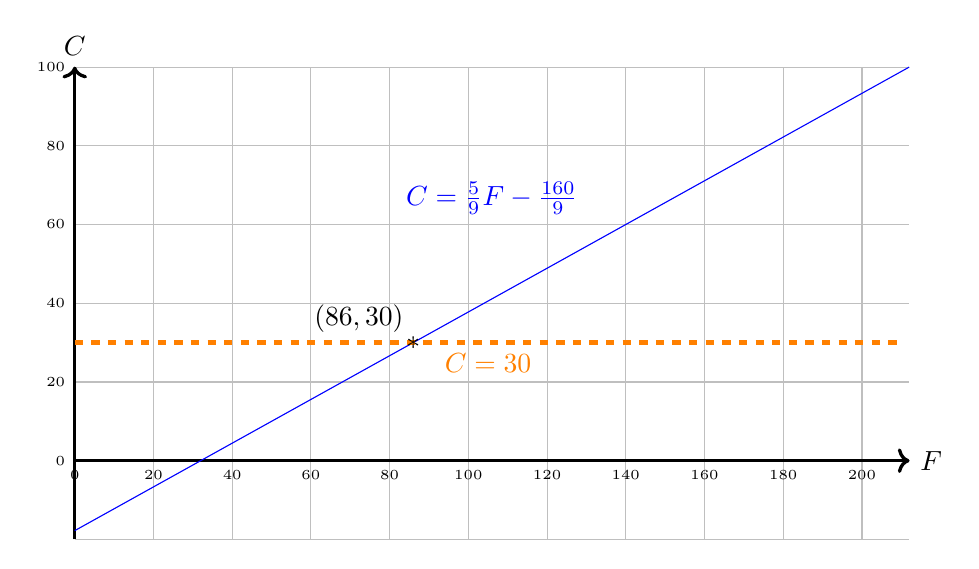
\begin{tikzpicture}[yscale=1/20, xscale=1/20][domain=-1:10]
    \draw[gray!50, thin, step=20] (0,-20) grid (212,100);
    \draw[very thick,->] (0,0) -- (212.1,0) node[right] {$F$};
    \draw[very thick,->] (0,-20) -- (0,100.1) node[above] {$C$};

    \foreach \x in {0,20,...,200} \draw (\x,0.05) -- (\x,-0.05) node[below] {\tiny\x};
    \foreach \y in {0,20,...,100} \draw (-0.05,\y) -- (0.05,\y) node[left] {\tiny\y};


    \draw[scale=1,domain=0:212,smooth,variable=\x,blue] plot ({\x},{(5/9)*\x-160/9});
  

\draw[blue] (106,60) --node[above]{$C=\frac{5}{9}F-\frac{160}{9}$}(106,60);
\draw[ultra thick, dashed, orange] (0,30) --node[below]{$C=30$} (210,30);

\node at (86,30){$*$};
\draw (86,30) --node[above left]{$(86,30)$}(86,30);



\end{tikzpicture}$$ 


\end{enumerate}

Desmos representation here: \url{https://www.desmos.com/calculator/tyoznzrk53}.


\end{example}

\begin{example}\label{Example:Proft}
\Q Suppose you were selling widgets for \$5 a unit, they have a marginal cost of \$3 per unit, and a fixed cost of production of \$20.

\begin{enumerate}
    \item Find the Cost, Revenue and Profit functions of producing $x$ widgets ($C(x), R(x), P(x)$) in dollars.
    \item For each widget sold, how much does your profit increase?
    \item  What is the cost of producing 30 widgets?
    \item What is the break even point?  (Zero profit).
\end{enumerate}

\Sol

\begin{enumerate}
    \item We break these down one at a time.
    \begin{enumerate}
        \item The marginal cost or cost per widget is \$3, and the cost for producing no widgets is the fixed cost of \$20.  Thus $C(x)=3x+20$.
        \item You get \$5 per widget sold, and clearly do not get any money for selling nothing, so $R(x)=5x+0=5x$.
        \item Profit is Revenue (money generated) minus Costs (money spent).  Thus $P(x)=R(x)-C(x)=5x-(3x+20)=2x-20$.
    \end{enumerate}
    $$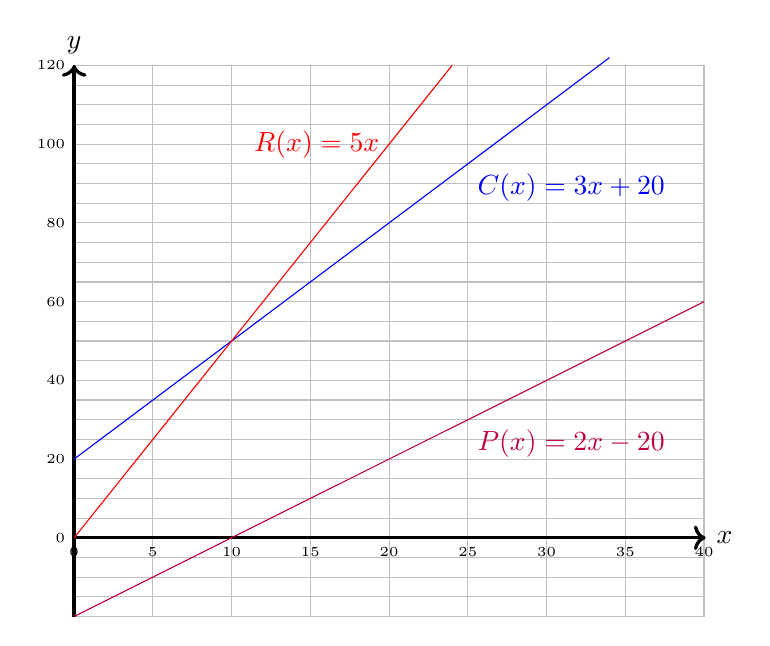
\begin{tikzpicture}[yscale=1/20, xscale=1/5]
    \draw[gray!50, thin, step=5] (0,-20) grid (40,120);
    \draw[very thick,->] (0,0) -- (40.1,0) node[right] {$x$};
    \draw[very thick,->] (0,-20) -- (0,120.1) node[above] {$y$};

    \foreach \x in {0,5,...,40} \draw (\x,0.05) -- (\x,-0.05) node[below] {\tiny\x};
    \foreach \y in {0,20,...,120} \draw (-0.05,\y) -- (0.05,\y) node[left] {\tiny\y};


    \draw[scale=1,domain=0:34,smooth,variable=\x,blue] plot ({\x},{3*\x+20});
  
    \draw[scale=1,domain=0:24,smooth,variable=\x,red] plot ({\x},{5*\x});

    \draw[scale=1,domain=0:40,smooth,variable=\x,purple] plot ({\x},{2*\x-20});

\draw[blue] (25,95) --node[below right]{$C(x)=3x+20$}(25,95);
\draw[red] (20,100) --node[left]{$R(x)=5x$}(20,100);
\draw[purple] (25,30) --node[below right]{$P(x)=2x-20$}(25,30);



\end{tikzpicture}$$ 

\url{https://www.desmos.com/calculator/d6l9b3kqho}

\item Since $P(x)=2x-20$, the change per unit of $x$ or profit per widget is the slope, or \$2/widget.

\item When you produce $\TCG{x=30}$ widgets, the cost will be:

\begin{eqnarray*}
C(x)&=&3x+20\\
C(x)&=&3\cdot\TCG{30}+20\\
C(x)&=&90+20\\
C(x)&=&110.\\
\end{eqnarray*}
The cost of producing 30 widgets is \$110.

 $$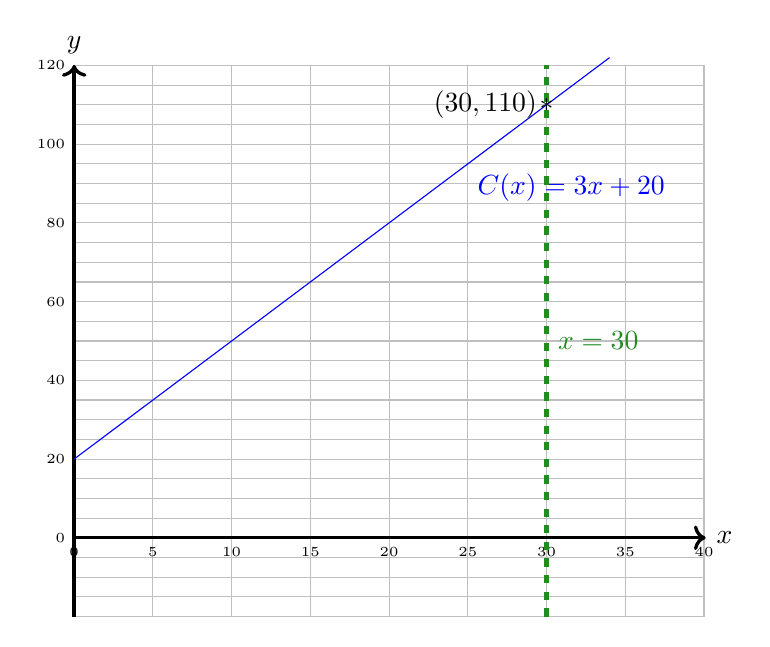
\begin{tikzpicture}[yscale=1/20, xscale=1/5]
    \draw[gray!50, thin, step=5] (0,-20) grid (40,120);
    \draw[very thick,->] (0,0) -- (40.1,0) node[right] {$x$};
    \draw[very thick,->] (0,-20) -- (0,120.1) node[above] {$y$};

    \foreach \x in {0,5,...,40} \draw (\x,0.05) -- (\x,-0.05) node[below] {\tiny\x};
    \foreach \y in {0,20,...,120} \draw (-0.05,\y) -- (0.05,\y) node[left] {\tiny\y};


    \draw[scale=1,domain=0:34,smooth,variable=\x,blue] plot ({\x},{3*\x+20});
  
%    \draw[scale=1,domain=0:24,smooth,variable=\x,red] plot ({\x},{5*\x});

%    \draw[scale=1,domain=0:40,smooth,variable=\x,purple] plot ({\x},{2*\x-20});

\draw[blue] (25,95) --node[below right]{$C(x)=3x+20$}(25,95);
%\draw[red] (20,100) --node[left]{$R(x)=5x$}(20,100);
%\draw[purple] (25,30) --node[below right]{$P(x)=2x-20$}(25,30);

\draw[ultra thick, dashed, ForestGreen] (30,-20) --node[right]{$x=30$} (30,120);

\node at (30,110){$*$};
\draw (30,110) --node[left]{$(30,110)$}(30,110);


\end{tikzpicture}$$ 
\url{https://www.desmos.com/calculator/cmoor2agyv}

\item The break even occurs when the profit is zero, $\TCO{P(x)=0}$.

\begin{eqnarray*}
P(x)&=&2x-20\\
\TCO{0}&=&2x-20\\
2x&=&20\\
x&=&10.
\end{eqnarray*}
The break even point occurs when $x=10$ widgets are sold.

 $$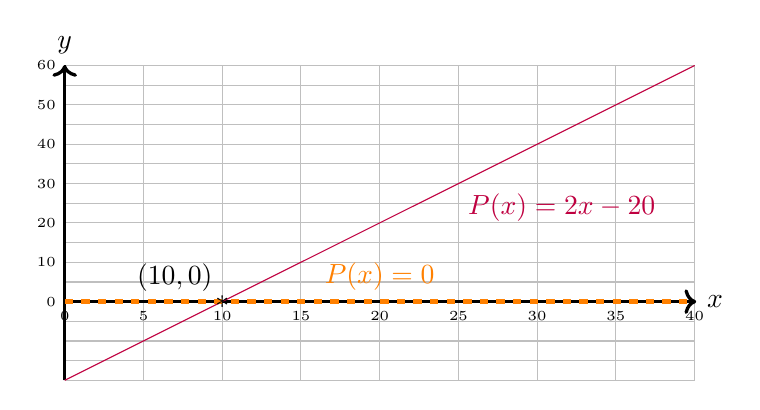
\begin{tikzpicture}[yscale=1/20, xscale=1/5]
    \draw[gray!50, thin, step=5] (0,-20) grid (40,60);
    \draw[very thick,->] (0,0) -- (40.1,0) node[right] {$x$};
    \draw[very thick,->] (0,-20) -- (0,60.1) node[above] {$y$};

    \foreach \x in {0,5,...,40} \draw (\x,0.05) -- (\x,-0.05) node[below] {\tiny\x};
    \foreach \y in {0,10,...,60} \draw (-0.05,\y) -- (0.05,\y) node[left] {\tiny\y};


%    \draw[scale=1,domain=0:34,smooth,variable=\x,blue] plot ({\x},{3*\x+20});
  
%    \draw[scale=1,domain=0:24,smooth,variable=\x,red] plot ({\x},{5*\x});

    \draw[scale=1,domain=0:40,smooth,variable=\x,purple] plot ({\x},{2*\x-20});

%\draw[blue] (25,95) --node[below right]{$C(x)=3x+20$}(25,95);
%\draw[red] (20,100) --node[left]{$R(x)=5x$}(20,100);
\draw[purple] (25,30) --node[below right]{$P(x)=2x-20$}(25,30);

\draw[ultra thick, dashed, orange] (0,0) --node[above]{$P(x)=0$} (40,0);

\node at (10,0){$*$};
\draw (10,0) --node[above left]{$(10,0)$}(10,0);


\end{tikzpicture}$$ 
\url{https://www.desmos.com/calculator/bdtdeqzqqa}

\end{enumerate}



\end{example}



\begin{example}
\Q Dr.\ Johnson is traveling to visit her mother for a holiday.  She drives at a constant speed of 75 mph.  After 3 hours, she passes a landmark that she knows is 200 miles from her mom's house.
\begin{enumerate}
    \item Find a function $D(t)$ that gives Dr.\ Johnson's distance to her mother house, in miles, after $t$ hours.
    \item How far away was she when she started driving?
    \item How many hours did it take from start to finish to complete this drive?
\end{enumerate}

\Sol 
\begin{enumerate}
    \item Since she is driving towards her mom's house, the distance from her to the house decreases at a rate of 75 miles per hour.  Thus $\TCR{m=-75}$.  At $t=3$ hours, her distance was 200 miles away.  Thus $\TCB{(3,200)}$ falls on the line representing this function.  Recall the techniques from Examples \ref{Example:PandS}, \ref{Example:PandSagain}.
     \begin{eqnarray*}
    D(t)&=&-75t+b\\
    \TCB{200}&=&\TCR{-75}\cdot\TCB{3}+b\\
    200&=&-225+b\\
    b&=&200+225=425.
    \end{eqnarray*}
    Thus $D(t)=-75t+425$.   
 $$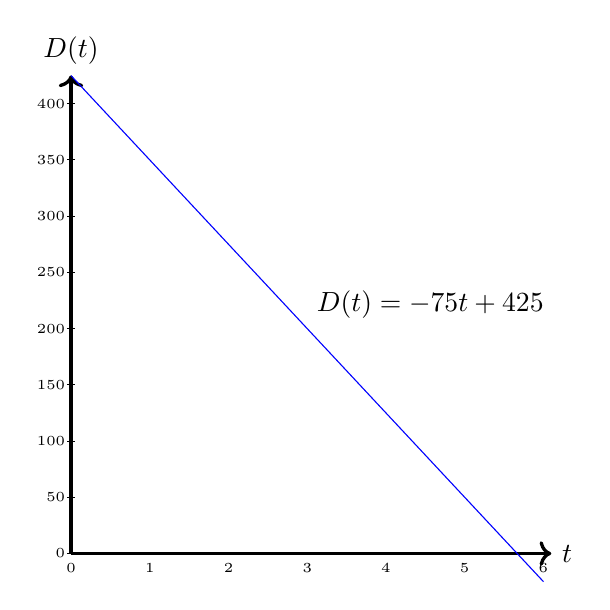
\begin{tikzpicture}[yscale=1/70]
    %\draw[gray!50, thin, step=5] (0,-20) grid (40,60);
    \draw[very thick,->] (0,0) -- (6.1,0) node[right] {$t$};
    \draw[very thick,->] (0,0) -- (0,425.1) node[above] {$D(t)$};

    \foreach \x in {0,1,...,6} \draw (\x,0.05) -- (\x,-0.05) node[below] {\tiny\x};
    \foreach \y in {0,50,...,425} \draw (-0.05,\y) -- (0.05,\y) node[left] {\tiny\y};



    \draw[scale=1,domain=0:6,smooth,variable=\x,blue] plot ({\x},{-75*\x+425});

\draw (3,200) --node[above right]{$D(t)=-75t+425$}(3,200);


%\node at (10,0){$*$};
%\draw (10,0) --node[above left]{$(10,0)$}(10,0);


\end{tikzpicture}$$ 
\url{https://www.desmos.com/calculator/uoul2cdsjs}
    \item At the start of the journey, $\TCG{t=0}$, and so she was $D(\TCG{0})=-75\cdot\TCG{0}+425=425$ miles from her mother's house.
\url{https://www.desmos.com/calculator/xuzh7xcgwk}    
    \item When she arrives, her distance from her mothers house is $\TCO{D(t)=0}$ miles and so:
     \begin{eqnarray*}
    D(t)&=&-75t+425\\
    \TCO{0}&=&-75t+425\\
    75t&=&425\\
    t&=&\frac{425}{75}\approx 5.6667.
    \end{eqnarray*}
So the trip takes $t=\frac{425}{75}\approx 5.6667$ hours or 5 hours and 40 minutes.    
 
$$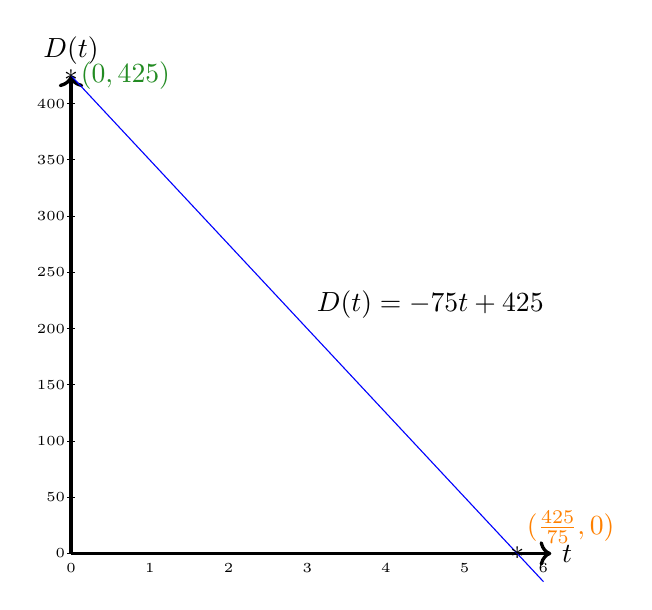
\begin{tikzpicture}[yscale=1/70]
    %\draw[gray!50, thin, step=5] (0,-20) grid (40,60);
    \draw[very thick,->] (0,0) -- (6.1,0) node[right] {$t$};
    \draw[very thick,->] (0,0) -- (0,425.1) node[above] {$D(t)$};

    \foreach \x in {0,1,...,6} \draw (\x,0.05) -- (\x,-0.05) node[below] {\tiny\x};
    \foreach \y in {0,50,...,425} \draw (-0.05,\y) -- (0.05,\y) node[left] {\tiny\y};



    \draw[scale=1,domain=0:6,smooth,variable=\x,blue] plot ({\x},{-75*\x+425});

\draw (3,200) --node[above right]{$D(t)=-75t+425$}(3,200);


\node at (0,425){$*$};
\draw[ForestGreen] (0,425) --node[right]{$(0,425)$}(0,425);

\node at (17/3,0){$*$};
\draw[orange] (17/3,0) --node[above right]{$(\frac{425}{75},0)$}(17/3,0);


\end{tikzpicture}$$  
 \url{https://www.desmos.com/calculator/dilrensiar}
    
\end{enumerate}


\end{example}


\begin{example}\label{Example:}
\Q Consider the following graphs of functions $q=S(p), D(p)$, where $p$ is the price of a product, and $q$ is the quantity demanded.

$$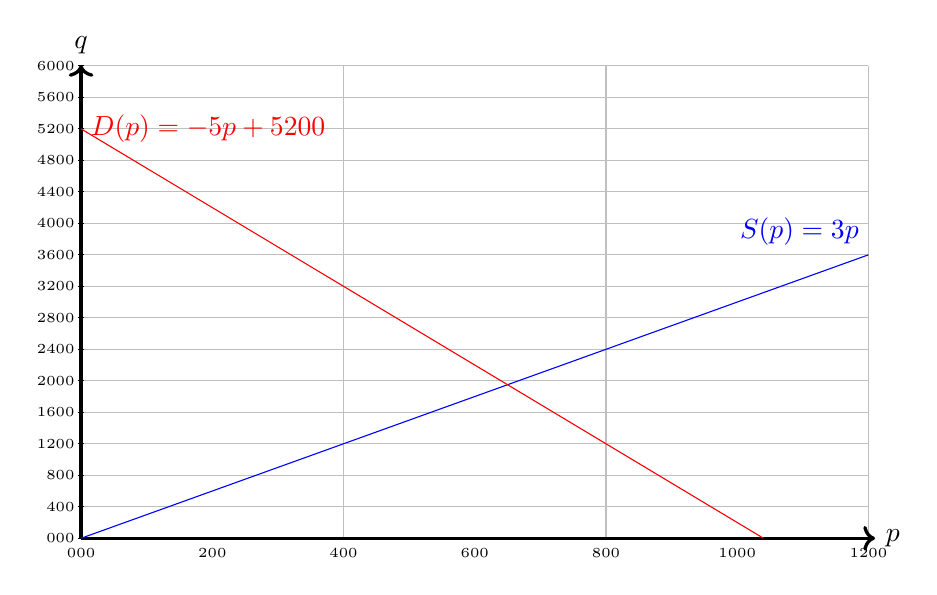
\begin{tikzpicture}[yscale=6/60, xscale=10/12]
    \draw[gray!50, thin, step=4] (0,0) grid (12,60);
    \draw[very thick,->] (0,0) -- (12.1,0) node[right] {$p$};
    \draw[very thick,->] (0,0) -- (0,60.1) node[above] {$q$};

    \foreach \x in {0,2,...,12} \draw (\x,0.05) -- (\x,-0.05) node[below] {\tiny\x00};
    \foreach \y in {0,4,...,60} \draw (-0.05,\y) -- (0.05,\y) node[left] {\tiny\y00};



    \draw[scale=1,domain=0:12,smooth,variable=\x,blue] plot ({\x},{3*\x});

    \draw[scale=1,domain=0:10.4,smooth,variable=\x,red] plot ({\x},{-5*\x+52});

\draw[red] (0,52) --node[right]{$D(p)=-5p+5200$}(0,52);
\draw[blue] (12,36) --node[above left]{$S(p)=3p$}(12,36);



\end{tikzpicture}$$

\begin{enumerate}
    \item Find the equations for the supply and demand curves $q=S(p), q=D(p)$, where $p$ is the price in dollars and $q$ is the quantity, either demanded or supplied.
    \item If \$350 is charged for this product, What is the surplus or deficit of products produced?
    \item Where is the equilibrium point (where supply and demand are the same)?
\end{enumerate}

\Sol

\begin{enumerate}
    \item It helps if we can identify some points on these lines.  We will work on them one at a time.
    \begin{enumerate}
        \item Graphically, we can see that $S(0)=0$, thus $(0,0)$ is on the supply line.  This also tells us the $q$-intercept, $b=0$.  We can also see that when $p=400, S(400)=1200$, thus $(400,1200)$ is also on this line.  Thus: $$m=\frac{1200-0}{400-0}=3.$$  So $S(p)=3p$.
        
        \item Graphically, we can see that $D(0)=5200$, thus $(0,5200)$ is on the demand line.  This also tells us the $q$-intercept, $b=5200$.  We can also see that when $p=400, D(400)=3200$, thus $(400,3200)$ is also on this line.  Thus: $$m=\frac{3200-5200}{400-0}=\frac{-2000}{400}=-5.$$  So $D(p)=-5p+5200$.
    \end{enumerate}
    \item When $p=350$, we will have $S(350)=3*350=1050$ products supplied, but $D(350)=-5*250+5200=3450$ demanded.  Thus there is a deficit of $3450-1050=2400$ products demanded that are not supplied, since demand exceeds supply.
    $$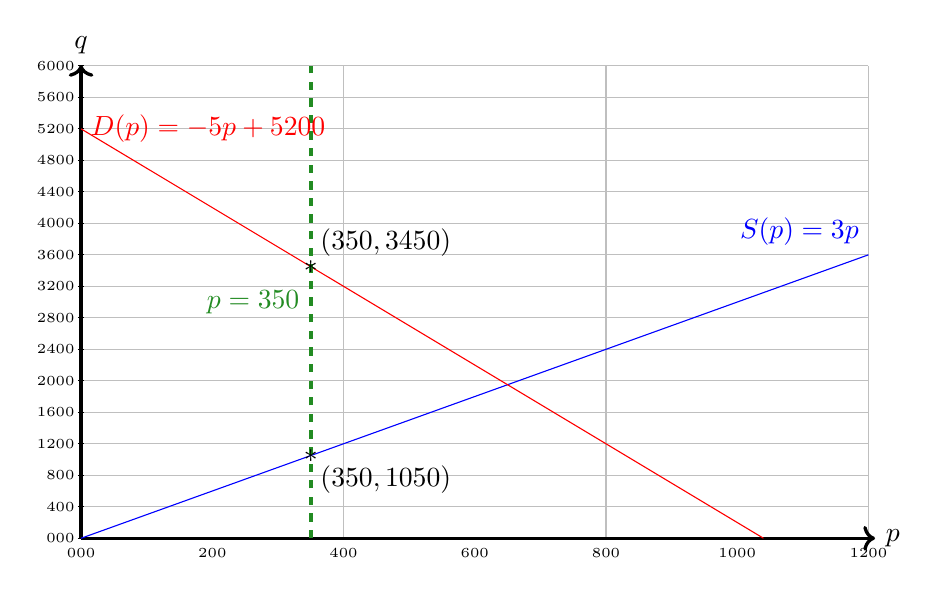
\begin{tikzpicture}[yscale=6/60, xscale=10/12]
    \draw[gray!50, thin, step=4] (0,0) grid (12,60);
    \draw[very thick,->] (0,0) -- (12.1,0) node[right] {$p$};
    \draw[very thick,->] (0,0) -- (0,60.1) node[above] {$q$};

    \foreach \x in {0,2,...,12} \draw (\x,0.05) -- (\x,-0.05) node[below] {\tiny\x00};
    \foreach \y in {0,4,...,60} \draw (-0.05,\y) -- (0.05,\y) node[left] {\tiny\y00};



    \draw[scale=1,domain=0:12,smooth,variable=\x,blue] plot ({\x},{3*\x});

    \draw[scale=1,domain=0:10.4,smooth,variable=\x,red] plot ({\x},{-5*\x+52});

    \draw[dashed, ultra thick, ForestGreen] (3.5,0) --node[left]{$p=350$} (3.5,60);

    \draw[red] (0,52) --node[right]{$D(p)=-5p+5200$}(0,52);
    \draw[blue] (12,36) --node[above left]{$S(p)=3p$}(12,36);
    
    \node at (3.5,34.5){$*$};
\draw (3.5,34.5) --node[above right]{$(350,3450)$}(3.5,34.5);

    \node at (3.5,10.5){$*$};
\draw (3.5,10.5) --node[below right]{$(350,1050)$}(3.5,10.5);


\end{tikzpicture}$$
\url{https://www.desmos.com/calculator/dee7rqh07j}

\item The equilibrium point is the point where the quantity supplied and demanded are the same.  Algebraically, this means $D(p)=S(p)$, and so:

\begin{eqnarray*}
-5p+5200&=&3p\\
5200&=&8p\\
p&=&\frac{5200}{8}=650.
\end{eqnarray*}

So the equilibrium happens when $p=650$ that is \$650 per unit.  Then, we note that $S(650)=3*650=1950$ and $D(p)=-5*650+5200=1950$, so the equilibrium point is $(650, 1950)$ or $\$650$ per unit, and 1950 units sold.

$$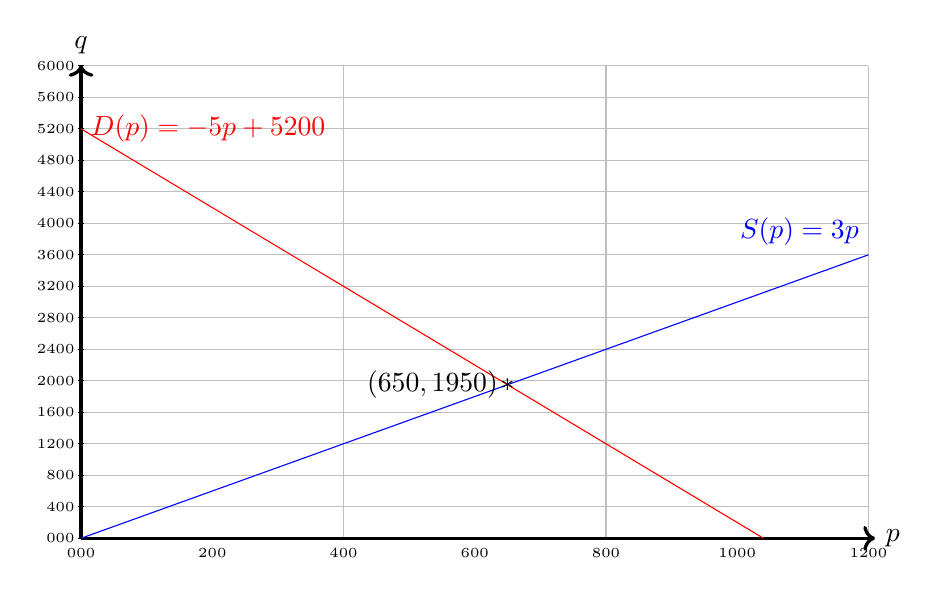
\begin{tikzpicture}[yscale=6/60, xscale=10/12]
    \draw[gray!50, thin, step=4] (0,0) grid (12,60);
    \draw[very thick,->] (0,0) -- (12.1,0) node[right] {$p$};
    \draw[very thick,->] (0,0) -- (0,60.1) node[above] {$q$};

    \foreach \x in {0,2,...,12} \draw (\x,0.05) -- (\x,-0.05) node[below] {\tiny\x00};
    \foreach \y in {0,4,...,60} \draw (-0.05,\y) -- (0.05,\y) node[left] {\tiny\y00};



    \draw[scale=1,domain=0:12,smooth,variable=\x,blue] plot ({\x},{3*\x});

    \draw[scale=1,domain=0:10.4,smooth,variable=\x,red] plot ({\x},{-5*\x+52});

\draw[red] (0,52) --node[right]{$D(p)=-5p+5200$}(0,52);
\draw[blue] (12,36) --node[above left]{$S(p)=3p$}(12,36);

    \node at (6.5,19.5){$*$};
\draw (6.5,19.5) --node[left]{$(650,1950)$}(6.5,19.5);



\end{tikzpicture}$$
\url{https://www.desmos.com/calculator/aywru3gvxu}
\end{enumerate}

\end{example}

These examples barely scratch the surface on how linear functions may be applied, but hopefully they gave you some sense on what sort of things they can be used to model, what sort of questions one can answer with them, and how to address them when the time comes.

\section{Linear Regression}\label{Section:LinearRegression}


\subsection{Philosophy of Linear Regression}

It turns out that it's fairly rare to find variables in the world that are truly independent of each other.  The world is full of variables that have hidden connections and part of understanding the universe we exist in is uncovering all these connections.  This is true since the first cave person stood near a fire and realized that standing near a fire made them warmer, thus uncovering a connection between standing near fires and warmth.\\

However, since the world is an interconnected web of hidden influences, it's rare to see two variables that can be solely and completely determined by one another.  In the example of our erstwhile caveperson, it's certain that standing near fire could make you warm, but so could standing in sunlight, so could wearing more furs.  There are a lot of factors that go into determining warmth besides proximity to flames.\\

Our goal here then is to take observations and determine whether or not they are connected, and what the connection is so we could potentially use one as a predictor for the other.  But moreover, we also want to measure how strong this connection is so that we can asses how accurate these predictions might be, and what other variables may be influencing these outcomes.


\subsection{Basic Mechanics of Linear Regression}

Wee begin with an illustrative example.

\begin{example}\label{Example:BasicRegression}

\Q Consider the data set:

$$\begin{array}{c|c}
x&y\\
\hline
1&2\\
2&2\\
3&4\\
4&4\\
5&6
\end{array}$$


If we were to plot this data, it would look like:

$$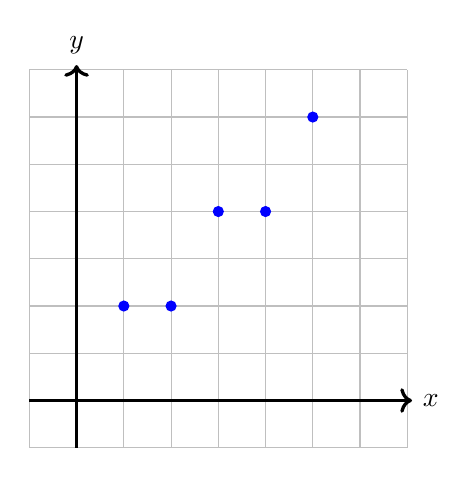
\begin{tikzpicture}[scale=.6][domain=-1:7]
    \draw[gray!50, thin, step=1] (-1,-1) grid (7,7);
    \draw[very thick,->] (-1,0) -- (7.1,0) node[right] {$x$};
    \draw[very thick,->] (0,-1) -- (0,7.1) node[above] {$y$};

%    \foreach \x in {-4,...,10} \draw (\x,0.05) -- (\x,-0.05) node[below] {\tiny\x};
%    \foreach \y in {-2,...,2} \draw (-0.05,\y) -- (0.05,\y) node[right] {\tiny\y};

\draw[blue, fill] (1,2) circle (3pt);
\draw[blue, fill] (2,2) circle (3pt);
\draw[blue, fill] (3,4) circle (3pt);
\draw[blue, fill] (4,4) circle (3pt);
\draw[blue, fill] (5,6) circle (3pt);

%  \draw[scale=1,domain=-2:2,smooth,variable=\x,blue] plot ({\x},{\x*\x*\x-3*\x}) node[above]{$y=f(x)$};


\end{tikzpicture}$$ % of mbox

Our goal here is to find a linear relationship between $x$ and $y$.  Graphically that means we want to draw a line that best fits the data we present here.  Of course, there is no line that can pass through all these points.  Our goal is to find the line that best fits these points, and to measure how well this line predicts actual values from the data.\\

\end{example}


We now commence with listing the basic arithmetic mechanics for finding a regression line.  Note that demonstrating why these formulations generate the best-fit line is beyond the scope of this text.  The most important thing to remember is: \\

``Given a bunch of points $(x_1, y_1), \ldots, (x_n, y_n)$, and a linear equation $\ell(x)=mx+b$ the \textbf{error} of each point is $e_i=\ell(x_i)-y_i$, that is the difference between the actual $y$ values, and what $\ell$ predicts should bee the $y$ values.  We are trying to find $m, b$ so that the sum of the errors squared $\sum e_i^2$ is minimized."\\

Why minimize $\sum e_i^2$?  Squaring the data erases the distinction between positive and negative error, between  over and under shoot.  Then, we want the total accumalated data to be as small as possible.




\begin{itemize}
\item $SS_X=\sum(x_i-\bar{x})^2=\sum x_i^2-\frac{(\sum x_i)^2}{n}$
\item $SS_Y=\sum(y_i-\bar{y})^2=\sum y_i^2-\frac{(\sum y_i)^2}{n}$
\item $SS_{XY}=\sum(x_i-\bar{x})(y_i-\bar{y})=\sum x_iy_i-\frac{(\sum x_i)(\sum y_i)}{n}$
\end{itemize}

The slope of the regression line will be:

$$\beta_1:=\frac{SS_{XY}}{SS_{X}}$$

If we recall, a line needs not just a slope, but a $y$ intercept.  So how can we figure out what the $y$ intercept should be?  Well, given the slope $\beta_1$, ON AVERAGE, given some $x_i$, we should get that $y_i=\beta_1x_i+\beta_0$, where $\beta_0$ is our yet-unknown $y$-intercept.  Again, this won't happen every time, or possibly ever, but it should be the average result, so the way we find $\beta_0$ is:

\begin{eqnarray*}
\bar{y}&=&\beta_1\bar{x}+\beta_0\\
\beta_0&=&\bar{y}-\beta_1\bar{x}.
\end{eqnarray*}

The above constructions are necessary to produce the best fit line.  In order to measure how good of a fit this line is, we introduce the \textbf{correlation coefficient}, usually denoted $r$.  This value is computed as follows:

$$r=\frac{n(\sum x_iy_i)-(\sum x_i)(\sum y_i)}{\sqrt{(n\sum x_i^2) - (\sum x_i)^2}\cdot \sqrt{n(\sum y_i^2)-(\sum y_i)^2}}.$$

This value measures the correction between the $x$ and $y$ values, with $r$ ranging from $-1$ to $1$.  The way we should interpret the $r$ values is as follows:

\begin{enumerate}
    \item Positive $r$ means positive correlation, meaning as $x$ goes up, $y$ tends to go up.  Negative $r$ means the opposite, as $x$ goes up, $y$ tends to go down.  Correlation of 0 means $x$'s change does not predict whether or not $y$ goes up or down.
    
    \item The closer $r$ is to 0, the weaker the correlation, meaning the ability to predict $y$ from $x$ is weak, the closer to $-1$ or $1$, the better our ability to predict $y$ from $x$.
\end{enumerate}

\begin{example}\label{Example:visualizecorr}
Consider the following plots of points.  Whether the points tend to have an upward or downward trend determines the sign of $r$, how well the best fit line predicts the points determines how close $r$ is to either $-1$ or $1$.

$$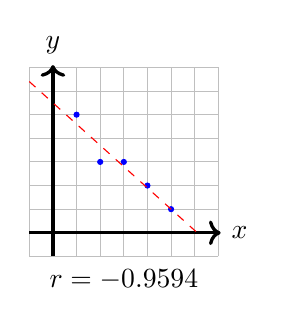
\begin{tikzpicture}[scale=.3][domain=-1:7]
    \draw[gray!50, thin, step=1] (-1,-1) grid (7,7);
    \draw[very thick,->] (-1,0) -- (7.1,0) node[right] {$x$};
    \draw[very thick,->] (0,-1) -- (0,7.1) node[above] {$y$};

%    \foreach \x in {-4,...,10} \draw (\x,0.05) -- (\x,-0.05) node[below] {\tiny\x};
%    \foreach \y in {-2,...,2} \draw (-0.05,\y) -- (0.05,\y) node[right] {\tiny\y};

\draw[blue, fill] (1,5) circle (3pt);
\draw[blue, fill] (2,3) circle (3pt);
\draw[blue, fill] (3,3) circle (3pt);
\draw[blue, fill] (4,2) circle (3pt);
\draw[blue, fill] (5,1) circle (3pt);

  \draw[scale=1,domain=-1:6.111,smooth,variable=\x,red, dashed] plot ({\x},{-0.9*\x+5.5});

\draw (3, -2) --node{$r=-0.9594$} (3,-2);

\end{tikzpicture}
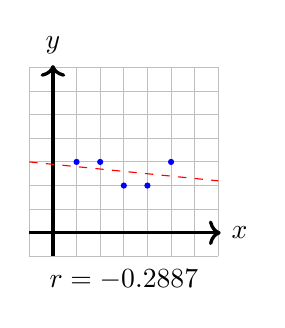
\begin{tikzpicture}[scale=.3][domain=-1:7]
    \draw[gray!50, thin, step=1] (-1,-1) grid (7,7);
    \draw[very thick,->] (-1,0) -- (7.1,0) node[right] {$x$};
    \draw[very thick,->] (0,-1) -- (0,7.1) node[above] {$y$};

%    \foreach \x in {-4,...,10} \draw (\x,0.05) -- (\x,-0.05) node[below] {\tiny\x};
%    \foreach \y in {-2,...,2} \draw (-0.05,\y) -- (0.05,\y) node[right] {\tiny\y};

\draw[blue, fill] (1,3) circle (3pt);
\draw[blue, fill] (2,3) circle (3pt);
\draw[blue, fill] (3,2) circle (3pt);
\draw[blue, fill] (4,2) circle (3pt);
\draw[blue, fill] (5,3) circle (3pt);

  \draw[scale=1,domain=-1:7,smooth,variable=\x,red, dashed] plot ({\x},{-0.1*\x+2.9});

\draw (3, -2) --node{$r=-0.2887$} (3,-2);

\end{tikzpicture}
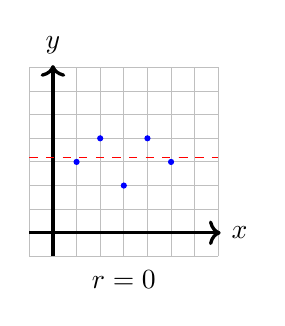
\begin{tikzpicture}[scale=.3][domain=-1:7]
    \draw[gray!50, thin, step=1] (-1,-1) grid (7,7);
    \draw[very thick,->] (-1,0) -- (7.1,0) node[right] {$x$};
    \draw[very thick,->] (0,-1) -- (0,7.1) node[above] {$y$};

%    \foreach \x in {-4,...,10} \draw (\x,0.05) -- (\x,-0.05) node[below] {\tiny\x};
%    \foreach \y in {-2,...,2} \draw (-0.05,\y) -- (0.05,\y) node[right] {\tiny\y};

\draw[blue, fill] (1,3) circle (3pt);
\draw[blue, fill] (2,4) circle (3pt);
\draw[blue, fill] (3,2) circle (3pt);
\draw[blue, fill] (4,4) circle (3pt);
\draw[blue, fill] (5,3) circle (3pt);

  \draw[scale=1,domain=-1:7,smooth,variable=\x,red, dashed] plot ({\x},{3.2});

\draw (3, -2) --node{$r=0$} (3,-2);

\end{tikzpicture}
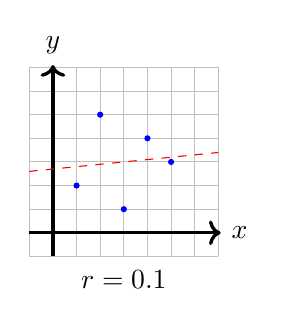
\begin{tikzpicture}[scale=.3][domain=-1:7]
    \draw[gray!50, thin, step=1] (-1,-1) grid (7,7);
    \draw[very thick,->] (-1,0) -- (7.1,0) node[right] {$x$};
    \draw[very thick,->] (0,-1) -- (0,7.1) node[above] {$y$};

%    \foreach \x in {-4,...,10} \draw (\x,0.05) -- (\x,-0.05) node[below] {\tiny\x};
%    \foreach \y in {-2,...,2} \draw (-0.05,\y) -- (0.05,\y) node[right] {\tiny\y};

\draw[blue, fill] (1,2) circle (3pt);
\draw[blue, fill] (2,5) circle (3pt);
\draw[blue, fill] (3,1) circle (3pt);
\draw[blue, fill] (4,4) circle (3pt);
\draw[blue, fill] (5,3) circle (3pt);

  \draw[scale=1,domain=-1:7,smooth,variable=\x,red, dashed] plot ({\x},{0.1*\x+2.7});

\draw (3, -2) --node{$r=0.1$} (3,-2);

\end{tikzpicture}
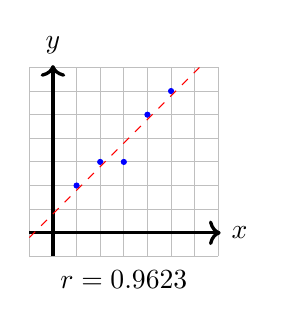
\begin{tikzpicture}[scale=.3][domain=-1:7]
    \draw[gray!50, thin, step=1] (-1,-1) grid (7,7);
    \draw[very thick,->] (-1,0) -- (7.1,0) node[right] {$x$};
    \draw[very thick,->] (0,-1) -- (0,7.1) node[above] {$y$};

%    \foreach \x in {-4,...,10} \draw (\x,0.05) -- (\x,-0.05) node[below] {\tiny\x};
%    \foreach \y in {-2,...,2} \draw (-0.05,\y) -- (0.05,\y) node[right] {\tiny\y};

\draw[blue, fill] (1,2) circle (3pt);
\draw[blue, fill] (2,3) circle (3pt);
\draw[blue, fill] (3,3) circle (3pt);
\draw[blue, fill] (4,5) circle (3pt);
\draw[blue, fill] (5,6) circle (3pt);

  \draw[scale=1,domain=-1:6.2,smooth,variable=\x,red, dashed] plot ({\x},{\x+0.8});

\draw (3, -2) --node{$r=0.9623$} (3,-2);

\end{tikzpicture}
$$
$$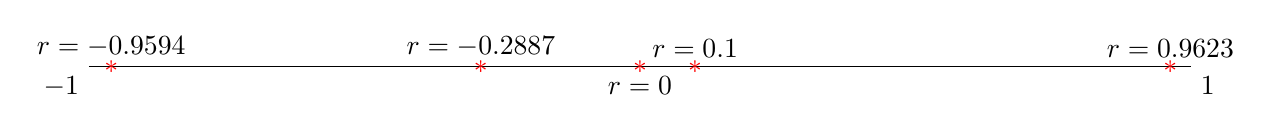
\begin{tikzpicture}[scale=7]
    \draw (-1,0)--(1,0);
    \draw (-1,0)--node[below left]{$-1$}(-1,0);
    \draw (1,0)--node[below right]{$1$}(1,0);  
    \draw[red]( 0.9623,0)--node{$*$}( 0.9623,0);
    \draw( 0.9623,0)--node[above]{$r=0.9623$}( 0.9623,0);
    \draw[red]( 0.1,0)--node{$*$}( 0.1,0);
    \draw( 0.1,0)--node[above]{$r=0.1$}( 0.1,0);
    \draw[red]( 0.0,0)--node{$*$}( 0.0,0);
    \draw( 0.0,0)--node[below]{$r=0$}( 0.0,0);
     \draw[red]( -0.2887,0)--node{$*$}( -0.2887,0);
    \draw( -0.2887,0)--node[above]{$r=-0.2887$}( -0.2887,0);
     \draw[red]( -0.9594,0)--node{$*$}( -0.9594,0);
    \draw( -0.9594,0)--node[above]{$r=-0.9594$}( -0.9594,0);
\end{tikzpicture}
$$
\end{example}

We further note that the closer $r$ is to either $-1, 1$ the closer $r^2$ is to 1, and similarly the closer $r$ is to 0, the closer $r^2$ is to 1.  Thus, we use $r^2$ as an overall measure of the strength of the correlation.  In fact, we say that $y$ is $r^2$ predicted by $x$, that is the values of $y$ are $r^2$ determinable by the values of $x$, the rest by other, as of yet undetermined variables.



\begin{example}\label{Example:BasicRegressionContd}
We continue from Example \ref{Example:BasicRegression}:

\begin{eqnarray*}
\bar{x}&=&\frac{1+2+3+4+5}{5}=3\\
\bar{y}&=&\frac{2+2+4+4+6}{5}=3.6\\
SS_X&=&(1-3)^2+(2-3)^2+(3-3)^2+(4-3)^2+(5-3)^2=10\\
SS_Y&=&(2-3.5)^2+(2-3.5)^2+(4-3.5)^2+(4-3.5)^2+(6-3.5)^2=11.25\\
SS_{XY}&=&(1-3)(2-3.5)+(2-3)(2-3.5)+(3-3)(4-3.5)+\\
&&(4-3)(4-3.5)+(5-3)(6-3.5)=10\\
\beta_1&=&\frac{10}{10}=1\\
\beta_0&=&3.6-(1)(3)=0.6
\end{eqnarray*}

So our best fit line is $y=1x+0.6$.



$$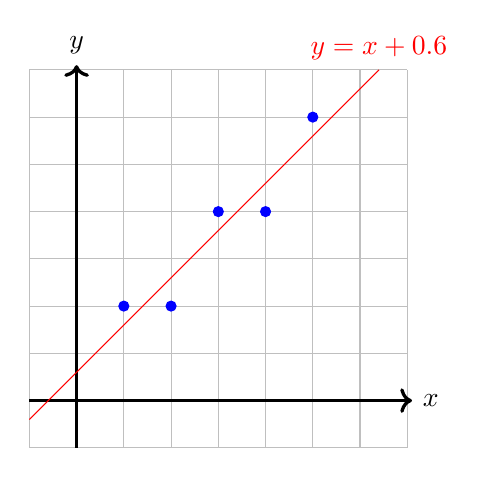
\begin{tikzpicture}[scale=.6][domain=-1:7]
    \draw[gray!50, thin, step=1] (-1,-1) grid (7,7);
    \draw[very thick,->] (-1,0) -- (7.1,0) node[right] {$x$};
    \draw[very thick,->] (0,-1) -- (0,7.1) node[above] {$y$};

%    \foreach \x in {-4,...,10} \draw (\x,0.05) -- (\x,-0.05) node[below] {\tiny\x};
%    \foreach \y in {-2,...,2} \draw (-0.05,\y) -- (0.05,\y) node[right] {\tiny\y};

\draw[blue, fill] (1,2) circle (3pt);
\draw[blue, fill] (2,2) circle (3pt);
\draw[blue, fill] (3,4) circle (3pt);
\draw[blue, fill] (4,4) circle (3pt);
\draw[blue, fill] (5,6) circle (3pt);

  \draw[scale=1,domain=-1:6.4,smooth,variable=\x,red] plot ({\x},{\x+0.6}) node[above]{$y=x+0.6$};


\end{tikzpicture}$$

Again, notice that none of the points actually fall on this line, but no possible line could have accomplished all of the points falling on it.  What we have instead is a line that passes through the points as closely as possible.  Define $e_i$ to be the error in prediction for $y_i$, that is let $e_i=y_i-(1\cdot x_i+0.6)$, then we see that:

\begin{eqnarray*}
e_1&=&2-(1+.6)=0.4\\
e_2&=&2-(2+.6)=-0.6\\
e_3&=&4-(3+.6)=0.4\\
e_4&=&4-(4+.6)=-0.6\\
e_5&=&6-(5+.6)=0.4
\end{eqnarray*}

$$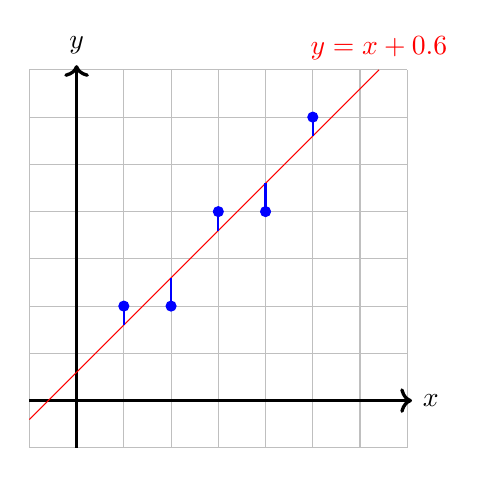
\begin{tikzpicture}[scale=.6][domain=-1:7]
    \draw[gray!50, thin, step=1] (-1,-1) grid (7,7);
    \draw[very thick,->] (-1,0) -- (7.1,0) node[right] {$x$};
    \draw[very thick,->] (0,-1) -- (0,7.1) node[above] {$y$};

%    \foreach \x in {-4,...,10} \draw (\x,0.05) -- (\x,-0.05) node[below] {\tiny\x};
%    \foreach \y in {-2,...,2} \draw (-0.05,\y) -- (0.05,\y) node[right] {\tiny\y};

\draw[blue, fill] (1,2) circle (3pt);
\draw[blue, fill] (2,2) circle (3pt);
\draw[blue, fill] (3,4) circle (3pt);
\draw[blue, fill] (4,4) circle (3pt);
\draw[blue, fill] (5,6) circle (3pt);

  \draw[scale=1,domain=-1:6.4,smooth,variable=\x,red] plot ({\x},{\x+0.6}) node[above]{$y=x+0.6$};

\draw[blue, thick](1, 1.6) -- (1,2);
\draw[blue, thick](2, 2.6) -- (2,2);
\draw[blue, thick](3, 3.6) -- (3,4);
\draw[blue, thick](4, 4.6) -- (4,4);
\draw[blue, thick](5, 5.6) -- (5,6);


\end{tikzpicture}$$


But $$e_1+e_2+e_3+e_4+e_5=(0.4)+(-0.6)+(0.4)+(0.6)+(0.4)=0.$$

This tells us this line passes through the ``middle" of the points.  Is it the best possible line?  Notice that $$\sum e_i^2=(0.4)^2+(-0.6)^2+(0.4)^2+(0.6)^2+(0.4)^2=1.2.$$  Is this the best we can do?  Again, a formal verification of this is beyond this text, but following this link: \url{https://www.desmos.com/calculator/gruczlkyyf}, you can see that by adjusting the parameters $m$ and $b$, that the sum of squares being 1.2 is the smallest error sum you can achieve.\\

To find $r$ we note that:

\begin{eqnarray*}
r&=&\frac{n(\sum x_iy_i)-(\sum x_i)(\sum y_i)}{\sqrt{(n\sum x_i^2) - (\sum x_i)^2}\cdot \sqrt{n(\sum y_i^2)-(\sum y_i)^2}}\\
&=&\frac{5(64)-(15)(18)}{\sqrt{5(55) - (15)^2}\cdot \sqrt{5(76)-(18)^2}}\\
&\approx&0.9449.
\end{eqnarray*}
So we can see that this fit is fairly close, and $x$ is a good predictor of $y$.  Since $r^2\approx 0.8929$, we can say that $y$'s value are 89.29\% determinable by $x$'s values.
\end{example}

\subsection{Good thing we don't live in the stone age.}

We should all agree that this was quite a lot of work to find these parameters for 5 values, and most data sets of work, have dozens, if not hundreds or thousands of data points.  It's simply impractical to do this by hand.\\

On the other hand a quick use of Desmos: \url{https://www.desmos.com/calculator/ir10f1wwzr} and entering the data points into the table, produces the best fit line, a plot, and the correlation coefficients.\\

Try entering your own data, adding or removing rows, and see how quickly and readily it will obtain our best fit lines and correlation coefficients!



\subsection{Applications}

\begin{example}
From fbi.gov from 2004-2013, the murder rates per 100,000 people are listed below:

$$\begin{array}{c|c}
\text{Years after 2000} & \text{Murders per 100,000 people}\\
x&y\\
\hline
4&5.5\\
5&5.6\\
6&5.8\\
7&5.7\\
8&5.4\\
9&5\\
10&4.8\\
11&4.7\\
12&4.7\\
13&4.5
\end{array}$$
\begin{enumerate}
\item Determine the best fit line for murders (per 100,000 people) $x$ years after 2000.
\item How much of a factor is the year in predictiung the number of murders?
\item Predict the murder rate in 2018.
\end{enumerate}

Entering this data in desmos: \url{https://www.desmos.com/calculator/em6xkq7udn}

\begin{enumerate}
\item It seems that the best fit line is $y=-0.144848x+6.40121$.
\item Since $r^2=0.8318$, we can say the murder rate is 83.18\% predictable by the year.
\item In 2018, the murder rate should be $-0.144848(18)+6.40121=3.793946$ or roughly 3.8 murders per 100,000 people in 2018.
\end{enumerate}




\end{example}



\begin{example}\label{Example:CorrQuizTest}
I personally wondered in quiz scores are a good predictor of test scores in Calculus.  I pulled out some data from this semester, and here are the average quiz and test scores of my students, anonymously of course:


$$\begin{array}{c|c}
\text{Quiz Average} & \text{Test Average}\\
x&y\\
\hline
87.5&100\\
76.13&94\\
75.83&93.5\\
53.53&83.5\\
76.13&83\\
71.13&78.85\\
56.13&76.5\\
73.57&70\\
66.13&69.5\\
66.13&63
\end{array}$$



\end{example}
\begin{enumerate}
\item Find the linear relationship between Quiz grades and Test grades.
\item Are Quiz grades a good predictor of Test grades?
\item If someone has an 80 average on Quizzes, predict their Test grade.
\end{enumerate}

So, once again:  \url{https://www.desmos.com/calculator/atipunytb1}

\begin{enumerate}
\item The relationship here is: $y=0.639883x+36.2168$, so there is a positive correlation, which we expect.
\item $r^2=0.2906$, so Test grades 29.06\% predictable by Quiz grades, which one would also expect, some people perform better in the Exam situation and some people perform worse.
\item We would have an expected test grade of $y=0.639883(80)+36.2168=87.40744$ or about 87.41\%.  But of course with an $r^2$ that small we shouldn't expect this to be terribly accurate.
\end{enumerate}


\subsection{Correlation $\neq$ Causation!}

A common misconception about correlated variables is that a strong correlation means that the $x$ variables \textbf{causes} the $y$ variable.  This is sometimes the case, but very often not true.\\

It is just as possible that $y$ causes $x$, or that $x$ and $y$ \textbf{share} common causes, or there's always complete coincidence.\\

In Example \ref{Example:CorrQuizTest}, if I had simply given everyone 100 on the quizzes without looking at them, and graded the exams in normal way, they likely would not have done any better.  One could argue that they would have done worse as a result.  So a positive correlation between the variables doesn't mean that one will rise simply by virtue of the other rising.\\

The bottom line is that correlations measure the strength and form of a relationship between variables, but not the nature of the relationship.











\chapter{Systems of Linear Equations and Matrices}


\section*{Introduction}

In this chapter, we introduce the notion of Linear Systems.  Linear Systems occur whenever we have collections of variables with linear relations with each other.  For example, we may want to eat a diet which contains certain levels of protein and fiber, and we wonder how much chicken and kale we should eat to achieve this?  Or we have Business, English and Math students, each of whom take different number of these courses, if we knew how many of each major there were, could we compute how many credits of each type of course would be taught?  This chapter will focus on the techniques and tools to model and address these types of situations.



\section{Systems of Linear  Equations}

A system of equations with unknowns $x_1,\ldots,x_n$ is a collection of first degree equations:

\begin{eqnarray*}
a_{1,1}x_1+a_{1,2}x_2+\cdots+a_{1,n}x_n&=&b_1\\
a_{2,1}x_1+a_{2,2}x_2+\cdots+a_{2,n}x_n&=&b_1\\
\vdots &=&\vdots\\
a_{m,1}x_1+a_{m,2}x_2+\cdots+a_{m,n}x_n&=&b_1\\
\end{eqnarray*}



\subsection{What Exactly is  a Solution to a System of Linear Equations?}

To answer the question that is the name of this section, we should kinda back up here and ask ``What is a solution to an equation?"\\

For example, what is a solution to $y=2x+3$? After dealing with linear equations in Chapter 1, we should have some sense as to what $y=2x+3$ looks like, that is a line with slope 2 and $y$-intercept $(0,3)$.  But what IS this line?  It's the collection of all points $(x,y)$ that make the above equation true.  So $(0,3), (-1,1)$ and $(2,7)$ are all on this line because they make the equation true ($3=2(0)+3, 1=2(-1)+3, 7=2(2)+3$).  A point like $(1,1)$ is NOT on this line because $1\neq 2(1)+3$.  \\

So a solution to an equation is \textbf{any point which makes the equation true}.\\

A \textit{System of Equations} is a collection of equations.  Thus, a solution to a system of equations is \textbf{any point which makes \underline{all} the equations true}.

\subsection{What are the Types of Solutions that we can have?}

So a solution to the system:

\begin{eqnarray*}
2x+3y&=&15\\
x-y&=&0
\end{eqnarray*}
is a collection of points that satisfy the first AND the second linear equalities.  The first equation describes the line: $y=-\frac{2}{3}x+5$, whereas the second describes the line $y=x$.  Each of these equations represent lines, so each individually has infinitely many solutions.  The question is, how many solutions do these lines have in common?\\

There are a number of ways to find out, but the most straight forward is simply to graph the system:

$$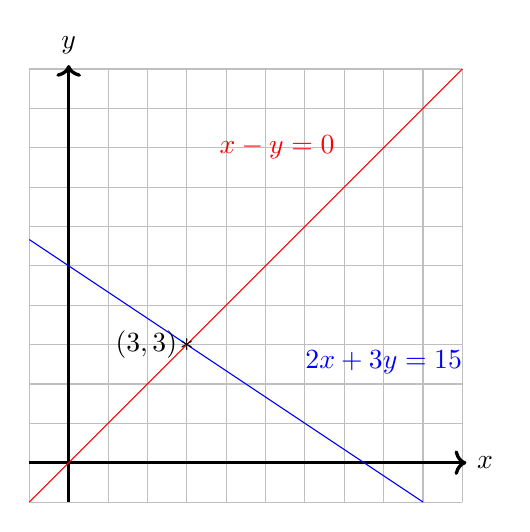
\begin{tikzpicture}[scale=0.5][domain=-1:10]
    \draw[gray!50, thin, step=1] (-1,-1) grid (10,10);
    \draw[very thick,->] (-1,0) -- (10.1,0) node[right] {$x$};
    \draw[very thick,->] (0,-1) -- (0,10.1) node[above] {$y$};

%    \foreach \x in {0,...,11} \draw (\x,0.05) -- (\x,-0.05) node[below] {\tiny\x};
%    \foreach \y in {0,...,28} \draw (-0.05,\y) -- (0.05,\y) node[right] {\tiny\y};


    \draw[scale=1,domain=-1:9,smooth,variable=\x,blue] plot ({\x},{(-2/3)*\x+5});
   \draw[scale=1,domain=-1:10,smooth,variable=\x,red] plot ({\x},{\x});

\node at (3,3){$*$};
\draw (3,3) --node[left]{$(3,3)$}(3,3);
\draw[blue] (8,2) --node[above]{$2x+3y=15$}(8,2);
\draw[red] (7,8) --node[left]{$x-y=0$}(7,8);



\end{tikzpicture}$$   


\url{https://www.desmos.com/calculator/cdrgyxm2al}.

As one can see, although each line has infinitely many points, the only solution they have in common is the point $(3,3)$.  To verify this, we note that $2(3)+3(3)=15$ and $3-3=0$, so both equations are satisfied.  This system has \textbf{a unique solution}\\

What else could happen when solving a system of equations?  Well, consider:


\begin{eqnarray*}
x+y&=&5\\
2x+2y&=&10.
\end{eqnarray*}

If we look at the graph of both lines, we only see one actual line:
 $$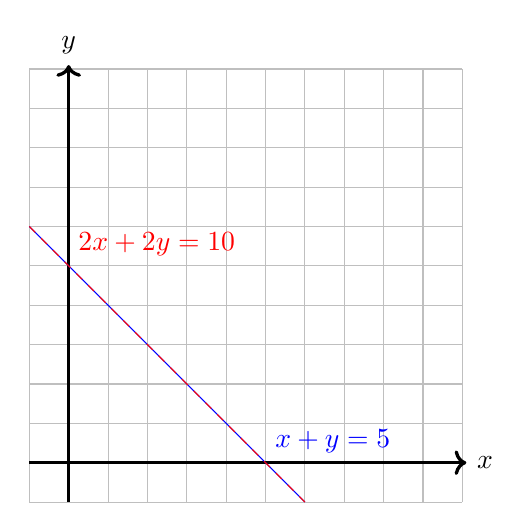
\begin{tikzpicture}[scale=0.5][domain=-1:10]
    \draw[gray!50, thin, step=1] (-1,-1) grid (10,10);
    \draw[very thick,->] (-1,0) -- (10.1,0) node[right] {$x$};
    \draw[very thick,->] (0,-1) -- (0,10.1) node[above] {$y$};

%    \foreach \x in {0,...,11} \draw (\x,0.05) -- (\x,-0.05) node[below] {\tiny\x};
%    \foreach \y in {0,...,28} \draw (-0.05,\y) -- (0.05,\y) node[right] {\tiny\y};


    \draw[scale=1,domain=-1:6,smooth,variable=\x,blue] plot ({\x},{(-1)*\x+5});
   \draw[scale=1,domain=-1:6,smooth,variable=\x,red, dashed] plot ({\x},{-1*\x+5});


\draw[blue] (5,0) --node[above right]{$x+y=5$}(5,0);
\draw[red] (0,5) --node[above right]{$2x+2y=10$}(0,5);


\end{tikzpicture}$$   


\url{https://www.desmos.com/calculator/oaqbrkruhl}. 

This is because both equations describe the same line.  After all, whenever $x+y=5$, it would have to be true that $2(x+y)=5\cdot2$ and thus $2x+2y=10$.  So ANY point that is a solution to one equation is a solution to the other, this system has \textbf{infinitely many solutions}.\\

Another possibility arises from the following example:


\begin{eqnarray*}
x+y&=&5\\
x+y&=&6\end{eqnarray*}

If we graph these lines side by side:

$$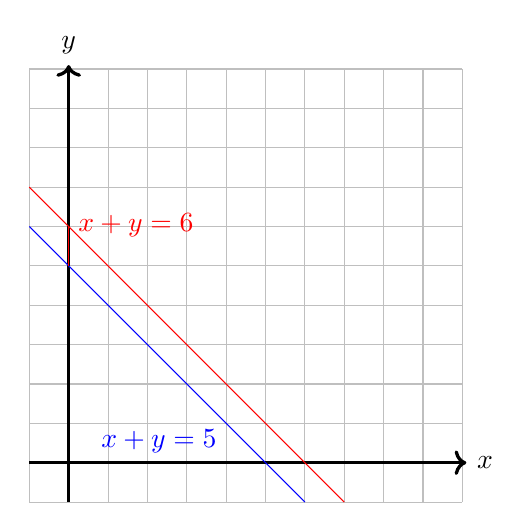
\begin{tikzpicture}[scale=0.5][domain=-1:10]
    \draw[gray!50, thin, step=1] (-1,-1) grid (10,10);
    \draw[very thick,->] (-1,0) -- (10.1,0) node[right] {$x$};
    \draw[very thick,->] (0,-1) -- (0,10.1) node[above] {$y$};

%    \foreach \x in {0,...,11} \draw (\x,0.05) -- (\x,-0.05) node[below] {\tiny\x};
%    \foreach \y in {0,...,28} \draw (-0.05,\y) -- (0.05,\y) node[right] {\tiny\y};


    \draw[scale=1,domain=-1:6,smooth,variable=\x,blue] plot ({\x},{(-1)*\x+5});
   \draw[scale=1,domain=-1:7,smooth,variable=\x,red] plot ({\x},{-1*\x+6});


\draw[blue] (4,0) --node[above left]{$x+y=5$}(4,0);
\draw[red] (0,6) --node[above right]{$x+y=6$}(0,5);


\end{tikzpicture}$$   


\url{https://www.desmos.com/calculator/djqxxge4ce}. 

We can see that these lines are parallel and do not actually have any points in common.  After all, how many pairs of numbers $x$ and $y$ sum to both 5 AND 6?  It should be clear that this system has \textbf{no solutions}.\\

Of course, these have all been Systems of Linear Equations in 2 variables.  When we increase the number of variables, we increase the dimensionality of the potential solution space, and what it means to be ``linear" changes somewhat.  Nevertheless, these examples illustrate the 3 possible outcomes of a system of linear equations in any dimension:

\begin{itemize}
\item There is a unique Solution.
\item There are infinitely many Solutions.
\item There are no Solutions.
\end{itemize}



\subsection{How do we find the Solution(s)/know we have No Solutions?}

In 2 variables, it's simple enough we can just graph, as we did above.  But we should try to develop some algebraic techniques as well, since this will be harder to do when we increase the dimensions of our problems.\\


What we introduce here is the Echelon Method, the general goal is to take non-zero multiples of our equations and use them to eliminate variables in the other equations so that a solution to a variable can be made known.  This process should also reveal if there are infinitely many or no solutions.\\


\begin{example}
\begin{eqnarray*}
2x+3y&=&1\\
x+y&=&0
\end{eqnarray*}

We note that whatever the solutions to this are, they should be the same as the solutions to:

\begin{eqnarray*}
x+\frac{3}{2}y&=&\frac{1}{2}\\
x+y&=&0
\end{eqnarray*}

We've divided the first equation in half, but we haven't actually changed what points will make that equation true.  Then:

\begin{eqnarray*}
x+\frac{3}{2}y&=&\frac{1}{2}\\
x+y-(x+\frac{3}{2}y)&=&0-\frac{1}{2}
\end{eqnarray*}

Must also be true, since we can add and subtract the same values from 2 sides of an equation and preserve the solutions.  By doing this, we kill off the $x$ in the second equation and we can solve for $y$:

\begin{eqnarray*}
x+\frac{3}{2}y&=&\frac{1}{2}\\
-\frac{1}{2}y&=&-\frac{1}{2}
\end{eqnarray*}

So $y=1$ based on the second line.  

\begin{eqnarray*}
x+\frac{3}{2}y&=&\frac{1}{2}\\
y&=&1
\end{eqnarray*}


If we take $-\frac{3}{2}$ times the second line and add it to the first:

\begin{eqnarray*}
x+\frac{3}{2}y-\frac{3}{2}(y)&=&\frac{1}{2}-\frac{3}{2}(1)\\
y&=&1
\end{eqnarray*}

We obtain:

\begin{eqnarray*}
x&=&-1\\
y&=&1
\end{eqnarray*}

We can verify that if we consider the original system:


\begin{eqnarray*}
2x+3y&=&1\\
x+y&=&0
\end{eqnarray*}
 then by evaluating at $x=-1, y=1$:
 
\begin{eqnarray*}
2(-1)+3(1)=-2+3&=&1\\
-1+1&=&0
\end{eqnarray*}
 


\end{example}

\begin{example} So if we consider:

\begin{eqnarray*}
x+y&=&2\\
2x+2y&=&4.
\end{eqnarray*}

Just like before, we want to kill the $x$ in the second equation:

\begin{eqnarray*}
x+y&=&2\\
2x+2y-2(x+y)&=&4-2(2).
\end{eqnarray*}

Which gives us:

\begin{eqnarray*}
x+y&=&2\\
0&=&0.
\end{eqnarray*}

Well..., certainly that second line doesn't contribute much, zero is always equal to itself.  So the solutions are just whenever $x+y=2$, which happens for infinitely many possible pairs.


\end{example}

\begin{example}


 Lastly, when we look at:

\begin{eqnarray*}
x+y&=&0\\
x+y&=&1.
\end{eqnarray*}

We can try to kill the $x$ in the second line as before:

\begin{eqnarray*}
x+y&=&0\\
x+y-(x+y)&=&1-0.
\end{eqnarray*}

Where we get:

\begin{eqnarray*}
x+y&=&0\\
0&=&1.
\end{eqnarray*}

So all you have to do is find a pair $(x,y)$ so that $0=1$... which is not ever going to happen.  So this will never have a solution.


\end{example}



\section{Representing a System of Linear Equations as a Matrix}

Given a system of equations, we can try to encode that information in a matrix:

So for example the system of equations:

\begin{eqnarray*}
2x+3y+z&=&3\\
-2x+4y+2z&=&0\\
x-y+2z&=&3
\end{eqnarray*}

Would have matrix representation:

$$ \left( \begin{array}{rrr|r}
2 & 3 & 1& 3\\
-2 & 4 & 2 & 0\\
1 & -1 & 2 & 3
\end{array}\right).$$

A \textbf{matrix} is a rectangular array of numbers, each number is an \textbf{entry} of the matrix.  In the above example, the vertical line is a visual reminder to separate the constant terms from the variables.  A matrix displayed this way is an \textbf{augmented matrix}.

By letting each column of a matrix represent a different variable or constant and arranging the linear equations into rows, one can write any linear system of equations as an augmented matrix.   Conversely, if you have a matrix:

$$ \left( \begin{array}{rr|r}
1 & 2 & 4\\
3 & 3  & 9\\
\end{array}\right)$$

This represent the system of equations:


\begin{eqnarray*}
x+2y&=&4\\
3x+3y&=&9
\end{eqnarray*}

\subsection{Solving Systems of Linear Equations}

So let's consider the above system/matrix:

$$ \left( \begin{array}{rr|r}
1 & 2 & 4\\
3 & 3  & 9\\
\end{array}\right)$$



We are allowed to manipulate this matrix in a number of ways.  Remembering that each row represents a linear equation:

\begin{enumerate}
\item \textbf{You can multiply any row by a non-zero multiple}.\\ 

We can do this because say, the solutions to $x+2y=4$ are the same as the solutions to $-x-2y=-4$ or $2x+4y=8$, so we're not adding in new solutions or removing existing solutions.

\item \textbf{You can add to any row, the multiple of any row.}\\

Adding a linear equality to another linear equality preserves the solutions to both equations.

\item \textbf{You can rearrange the rows.}\\

The solutions to a system of equations does not depend on the order in which they appear.

\end{enumerate}


So our goal here is to change this system into one where it's much easier to see what the solution is.  The best way to do this, is to not have all these x's and y's, I want 2 equations: $x=?, y=??$.

So:

\begin{eqnarray*}
\left( \begin{array}{rr|r}
1 & 2 & 4\\
3 & 3  & 9\\
\end{array}\right)&&\\
(1/3)R_2\mapsto R_2 \left( \begin{array}{rr|r}
1 & 2 & 4\\
1 & 1  & 3\\
\end{array}\right)&&\\
(-1)R_1+R_2\mapsto R_2 \left( \begin{array}{rr|r}
1 & 2 & 4\\
0 & -1  & -1\\
\end{array}\right)&&\\
(-1)R_2\mapsto R_2 \left( \begin{array}{rr|r}
1 & 2 & 4\\
0 & 1  & 1\\
\end{array}\right)&&\\
(-2)R_2+R_1\mapsto R_1 \left( \begin{array}{rr|r}
1 & 0 & 2\\
0 & 1  & 1\\
\end{array}\right)&&\\
\end{eqnarray*}





What system of equations of this?  It is:

\begin{eqnarray*}
x+0y&=&2\\
0x+y&=&1
\end{eqnarray*}

Which must mean: $x=2, y=1$, alright!  By the way, one can test your answers to see if they are correct!

$$1(2)+2(1)=4, 3(1)+3(2)=9$$ so it checks out.

A matrix with 1's across the diagonal, and 0's above and below these 1's (as above) is called \textbf{reduced row-echelon form}.  A process to obtain a reduced row echelon form matrix  is called the \textbf{Gauss-Jordan Method}.  The methodology is:

\begin{enumerate}
    \item Starting with the first row, multiply by a number so it's leading (leftmost) value is 1.
    \item Multiply and add copies of this row to all rows below so that every entry below this leading 1 is a 0.
    \item Repeat steps (1) and (2) for subsequent rows until the last row.
    \item Starting with the bottom row working up, repeat steps (1)-(3) except working upwards and making entries \textbf{above} the leading 1's 0.
\end{enumerate}

\begin{example}\label{Example:GaussJordan}
Solve the linear system:

\begin{eqnarray*}
3x+2y+z&=&1\\
x+y-z&=&3\\
2x-y+2z&=&-2\\
\end{eqnarray*}

This corresponds to augmented matrix:


$$\left( \begin{array}{rrr|r}
3 & 2 & 1 & 1\\
1 & 1  & -1 & 3\\
2 & -1 & 2 & -2
\end{array}\right)$$

So applying Gauss-Jordan:

\begin{eqnarray*}
\frac{1}{3}R_1\to R_1 \left( \begin{array}{rrr|r}
3 & 2 & 1 & 1\\
1 & 1  & -1 & 3\\
2 & -1 & 2 & -2
\end{array}\right)&&\\
\frac{1}{3}R_1\to R_1 \left( \begin{array}{rrr|r}
1 & \frac{2}{3} & \frac{1}{3} & \frac{1}{3}\\
1 & 1  & -1 & 3\\
2 & -1 & 2 & -2
\end{array}\right)&&\\
-1R_1+R_2\to R_2\left( \begin{array}{rrr|r}
1 & \frac{2}{3} & \frac{1}{3} & \frac{1}{3}\\
0 & -\frac{1}{3}  & -\frac{4}{3} & \frac{8}{3}\\
2 & -1 & 2 & -2
\end{array}\right)&&\\
-3R_2\to R_2\left( \begin{array}{rrr|r}
1 & \frac{2}{3} & \frac{1}{3} & \frac{1}{3}\\
0 & 1  & 4 & -8\\
2 & -1 & 2 & -2
\end{array}\right)&&\\
-2R_1+R_3\to R_3\left( \begin{array}{rrr|r}
1 & \frac{2}{3} & \frac{1}{3} & \frac{1}{3}\\
0 & 1  & 4 & -8\\
0 & -\frac{7}{3} & \frac{4}{3} & -\frac{8}{3}
\end{array}\right)&&\\
\frac{3}{7}R_2+R_3\to R_3\left( \begin{array}{rrr|r}
1 & \frac{2}{3} & \frac{1}{3} & \frac{1}{3}\\
0 & 1  & 4 & -8\\
0 & 0 & \frac{64}{21} & -\frac{128}{21}
\end{array}\right)&&\\
\frac{21}{64}R_3\to R_3\left( \begin{array}{rrr|r}
1 & \frac{2}{3} & \frac{1}{3} & \frac{1}{3}\\
0 & 1  & 4 & -8\\
0 & 0 & 1 & -2
\end{array}\right)&&\\
\end{eqnarray*}

Then we work from bottom back up:

\begin{eqnarray*}
-4R_3 + R_2\to R_2\left( \begin{array}{rrr|r}
1 & \frac{2}{3} & \frac{1}{3} & \frac{1}{3}\\
0 & 1  & 0 & 0\\
0 & 0 & 1 & -2
\end{array}\right)&&\\
-\frac{1}{3}R_3 + R_1\to R_1\left( \begin{array}{rrr|r}
1 & \frac{2}{3} & 0 & 1\\
0 & 1  & 0 & 0\\
0 & 0 & 1 & -2
\end{array}\right)&&\\
-\frac{2}{3}R_2 + R_1\to R_1\left( \begin{array}{rrr|r}
1 & 0 & 0 & 1\\
0 & 1  & 0 & 0\\
0 & 0 & 1 & -2
\end{array}\right)&&\\
\end{eqnarray*}

Which corresponds to the linear system:


\begin{eqnarray*}
1x+0y+0z&=&1\\
0x+1y+0z&=&0\\
0x+0y+z&=&-2\\
\end{eqnarray*}

Which has solution $x=1, y=0, z=2$.  To verify this works, we can check:

\begin{eqnarray*}
3(1)+2(0)+(-2)&=&1\\
(1)+(0)-(-2)&=&3\\
2(1)-(0)+2(-2)&=&-2\\
\end{eqnarray*}

and we have solved our linear system.


\end{example}

\subsection{Reduced Row Echelon Form using Technology.}

Suppose we wanted to solve the system associated with the augmented matrix:

$$ \left( \begin{array}{rrr|r}
2 & 3 & 1& 3\\
-2 & 4 & 2 & 0\\
1 & -1 & 2 & 3
\end{array}\right).$$

We could solve this the same way we did Example \ref{Example:GaussJordan}, but your first thought here is probably ``I don't want to do this."  Yeah, me neither.  One thing to note is that this process of finding a reduced row echelon form of a matrix is fairly mechanical.  So, we should be able to do this with a machine.

Following this link to an independent sagecell:  \url{https://sagecell.sagemath.org/?z=eJxztM1NLCnKrNAIDNRRiI420jHWMdQxjtWJ1jXSMdEx0jEAMg11dA2BTOPYWE1eroKizLwSDUcES6-oKDVNQ1MTAN6nE6M=&lang=sage}.  You see the following code:

\begin{verbatim}
A=matrix(QQ, [[2,3,1,3],[-2,4,2,0],[1,-1,2,3]])
print(A)
print(A.rref())
\end{verbatim}

The first line defines the matrix $A$ with the rows identical to the rows we defined in our above matrix.  Then the code returns a printout of that matrix, and it's reduced row echelon form:


$$ \left( \begin{array}{rrr|r}
1 & 0 & 0& 1\\
0 & 1 & 0 & 0\\
0 & 0 & 1 & 1
\end{array}\right)$$

So $x=1, y=0, z=1$.  Is this right?  Well, 

\begin{eqnarray*}
2(1)+3(0)+1&=&3\\
-2(1)+4(0)+2(1)&=&0\\
1-0+2(1)&=&3
\end{eqnarray*}

Works for me.

By the way, if you enter the matrix from Example \ref{Example:GaussJordan}, and replace the first line with:

\begin{verbatim}
A=matrix(QQ, [[3,2,1,1],[1,1,1,3],[2,-1,2,-2]])
\end{verbatim}

You should have the reduced row echelon matrix we achieved earlier.






\subsection{Infinitely many solutions}

Consider the system:


\begin{eqnarray*}
x+2y+z&=&3\\
-x+y+0z&=&0\\
0x+3y+z&=&3
\end{eqnarray*}

Then by using rref using as $A$:


\begin{verbatim}
A=matrix(QQ, [[1,2,1,3],[-1,1,0,0],[0,3,1,3]])
\end{verbatim}

We would obtain:


$$ \left( \begin{array}{rrr|r}
1 & 0 & 1/3& 1\\
0 & 1 & 1/3 & 1\\
0 & 0 & 0 & 0
\end{array}\right)$$

Which gives us the system:

\begin{eqnarray*}
x+0y+(1/3)z&=&1\\
0x+y+(1/3)z&=&1\\
0x+0y+0z&=&0\\
\end{eqnarray*}

Well, the last line is useless, it basically says that $0=0$, which is true but useless.  Let's break down the remaining equations:

\begin{eqnarray*}
x+(1/3)z&=&1\\
y+(1/3)z&=&1
\end{eqnarray*}

Which can be thought of as:

\begin{eqnarray*}
x&=&1-(1/3)z\\
y&=&1-(1/3)z
\end{eqnarray*}

So basically what this is saying, no matter what $z$ is, you can fin $x$ and $y$.  So if $z=0$, then $x,y=1$. But if $z=6$, then $x,y=-1$.  Well, what is $z$?  Apparently it can be whatever we want, both of the above triplets provide perfectly legitimate solutions to the original system.  What you see described is a line of solutions.  The 3 equations describe 3 planes in 3 dimensional ($x,y,z)$ space and they intersect at this line which can be describes as the solution to this equation.

\subsection{No Solutions}


Consider a similar system:



\begin{eqnarray*}
x+2y+z&=&3\\
-x+y+0z&=&0\\
0x+3y+z&=&0
\end{eqnarray*}

Then by using rref using as $A$:


\begin{verbatim}
A=matrix(QQ, [[1,2,1,3],[-1,1,0,0],[0,3,1,0]])
\end{verbatim}

We would obtain:


$$ \left( \begin{array}{rrr|r}
1 & 0 & 1/3& 1\\
0 & 1 & 1/3 & 1\\
0 & 0 & 0 & 0
\end{array}\right)$$

Which gives us the system:

\begin{eqnarray*}
x+0y+(1/3)z&=&1\\
0x+y+(1/3)z&=&1\\
0x+0y+0z&=&1\\
\end{eqnarray*}


Well, what does this last line mean?  It says that $0=1$.  When will this happen?  Well basically never, no choice of $x,y,z$ will ever make this true, our 3 planes do not intersect at a point or line or at all, so there is no solution.  


\subsection{Applications}

\begin{example}
A new airline has recently purchased a fleet of Airbus A330-300s, Boeing 767-300ERs, and Boeing Dreamliner 787-9s to meet an estimated demand for 9,300 seats. The A330-300s seat 330 passengers and cost \$250 million each, the 767-300ERs seat 270 passengers and cost \$200 million each, while the 787-9s seat 240 passengers and cost \$250 million each. The total cost of the fleet, which had twice as many 787-9s as 767s, was \$8,100 million. How many of each type of aircraft did the company purchase?\\

It helps perhaps if we organize some of this information in a table.

$$\begin{tabular}{|r||c|c|c||c|}
\hline
& A330-300s &  767-300ERs & 787-9s & Total\\
\hline
\hline
\textbf{Capacity} & 330 & 270 & 240 & \textbf{9,300}\\
\hline
\textbf{Cost (\$ million)} & 250 & 200 & 250 & \textbf{8,100}\\
\hline
\end{tabular}
$$

By letting $x$ denote the numbere of A330-300's, $y$ denote the number of 767-300ERs and $z$ denote the number of 787-9s, we obtain the following linear equalities:

First, the total capacity is 9,300 seats: $$330x+270y+240z=9300.$$

Next, the total cost is \$8,100 million: $$250x+200y+250z=8100.$$

Finally, there are twice as many 787-9s as 767-300ERs: %
\begin{eqnarray*}
z&=&2y\\
-2y+z&=&0.
\end{eqnarray*}

Giving us a system:

\begin{eqnarray*}
330x+270y+240z&=&9300\\
250x+200y+250z&=&8100\\
-2y+z&=&0
\end{eqnarray*}
and corresponding augmented matrix:

$$ \left( \begin{array}{rrr|r}
330 & 270 & 240& 9300\\
250 & 200 & 250 & 8100\\
0 & -2 & 1 & 0
\end{array}\right).$$

Using any method we'd like, we find row reduced echelon form:

$$ \left( \begin{array}{rrr|r}
1 & 0 & 0& 10\\
0 & 1 & 0 & 8\\
0 & 0 & 1 & 16
\end{array}\right)$$

which corresponds to $x=10, y=8, z=16$ or 10 A330-300s, 8 767300ERs and 16 787-9s.

To verify that this is a legitimate solution, check:

\begin{eqnarray*}
330(10)+270(8)+240(16)&=&9300\\
250(10)+200(8)+250(16)&=&8100\\
-2(8)+16&=&0.
\end{eqnarray*}



\end{example}


\begin{example}\label{Example:Vitamin}
Margo needs 200mg of vitamin A, 100mg of vitamin D, and 140mg of vitamin E per week. She has three supplements: the first contains 20\% vitamin A, 20\% vitamin D and 20\%
vitamin E; the second contains 10\% vitamin A, 30\% vitamin D and 40\% vitamin E; the third contains 50\% vitamin A, 10\% vitamin D and 20\% vitamin E. How much of each
supplement should she eat each week?\\

Let $x,y,z$ denote the quantities of supplements 1,2 and 3 she takes each week.  She needs 200mg of vitamin A, which gives us: $$0.2x+0.1y+0.5z=200.$$  Similarly, for 100mg of vitamin D: $$0.2x+0.3y+0.1z=100$$ and for 140mg of vitamin E: $$0.2x+0.2y+0.4z=140.$$

This gives us the system:


\begin{eqnarray*}
0.2x+0.1y+0.5z&=&200\\
0.2x+0.3y+0.1z&=&100\\
0.2x+0.4y+0.2z&=&140
\end{eqnarray*}
 with corresponding matrix:

$$ \left( \begin{array}{rrr|r}
0.2 & 0.1 & 0.5& 200\\
0.2 & 0.3 & 0.1 & 100\\
0.2 & 0.4 & 0.2 & 140
\end{array}\right).$$

This has reduced row echelon form:

$$ \left( \begin{array}{rrr|r}
1 & 0 & 0& 200\\
0 & 1 & 0 & 100\\
0 & 0 & 1 & 300
\end{array}\right)$$

which corresponds to solution $x=200, y=100, z=300$ or 200 mg of supplement 1, 100mg of supplement 2 and 300mg of supplement 3.


\end{example}


\begin{example}

Suppose an event with 300 people ends, and the attendees walk from the venue to two restaurants, Xavier's and Yoneda's. They walk along streets Anderson, Birmingham and Central, which are all one way.  When the night ends, there are 75 people and Xavier's and 225 at Yoneda's.

$$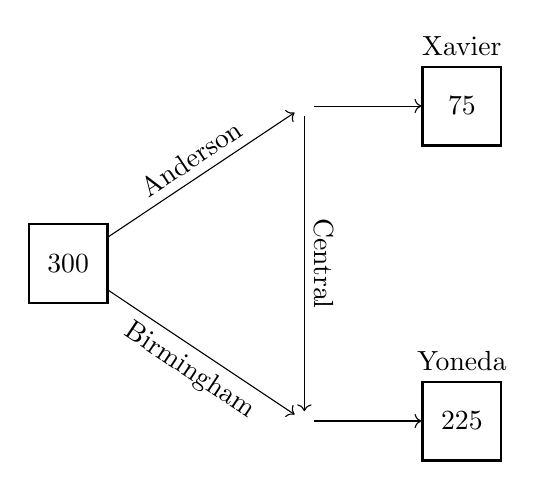
\begin{tikzpicture}
\node (V) at (0,0) [draw,thick,minimum width=1cm,minimum height=1cm] {$300$};

\node (I1) at (3,2) {};
\node (I2) at (3,-2) {};


\draw[->] (V) -- (I1)node[midway,sloped,above]{Anderson};;
\draw[->] (V) -- (I2) node[midway,sloped,below]{Birmingham};
\draw[->] (I1) -- (I2) node[midway,sloped,above]{Central};

\node[label={Xavier}] (X) at (5,2) [draw,thick,minimum width=1cm,minimum height=1cm] {75};

\node[label={Yoneda}] (Y) at (5,-2) [draw,thick,minimum width=1cm,minimum height=1cm] {225};

\draw[->] (I1)--(X);
\draw[->] (I2)--(Y);


\end{tikzpicture}$$

Let $a,b,c$ denote the number of people walking along Anderson, Birmingham and Central.

\begin{enumerate}
    \item Find an expression for the amount of people walking along each street.\\
    
    We first set up our systems of equations.  We first note that all 300 people have to walk either along either Anderson or Birmingham, so $$a+b=300.$$  Next, the 75 at Xavier is the however many people walked down Anderson, and take away whoever veered off onto Central so: $$a-c=75.$$  The 225 people at Yoneda is everyone coming across Birmingham and Central so $$b+c=225.$$  Thus the system is:
    
    \begin{eqnarray*}
    a+b&=&300\\
    a-c&=&75\\
    b+c&=&225,\\
    \end{eqnarray*}
    
    with associated augmented matrix:
    
    $$ \left( \begin{array}{rrr|r}
1 & 1 & 0& 300\\
1 & 0 & -1 & 75\\
0 & 1 & 1 & 225
\end{array}\right).$$
    
So the reduced row echelon form of this is:

    $$ \left( \begin{array}{rrr|r}
1 & 0 & -1 & 75\\
0 & 1 & 1 & 225\\
0 & 0 & 0& 0
\end{array}\right).$$

What this tells us is that there is not a unique solution, as the system associated with this matrix is:

    \begin{eqnarray*}
    a-c&=&75\\
    b+c&=&225,\\
    \end{eqnarray*}

Which is two of the original equations.  So, depending on what $c$ is, this will determine how many people traverse Anderson and Birmingham.

\item If 50 people crossed central, how many people crossed Anderson and Birmingham?\\

So letting $c=50$, we would have:

    \begin{eqnarray*}
    a-c&=&75\\
    a-50&=&75\\
    a&=&125\\
    b+c&=&225\\
    b+50&=&225\\
    b&=&175,
    \end{eqnarray*}
So 125 people across Anderson and 175 across Birmingham.\\

Another way to do this would be to add an equation $c=50$ to our system:

$$ \left( \begin{array}{rrr|r}
1 & 1 & 0& 300\\
1 & 0 & -1 & 75\\
0 & 1 & 1 & 225\\
0 & 0 & 1 & 50
\end{array}\right).$$
    
    Which has reduced row echelon form:
 
 $$ \left( \begin{array}{rrr|r}
1 & 0 & 0 & 125\\
0 & 1 & 0 & 175\\
0 & 0 & 1& 50\\
0 & 0 & 0& 0
\end{array}\right).$$   

That is $a=125, b=125, c=50$ which is our solution above.

\item If 100 people go through Anderson, how many go through Birmingham or Central?\\

We can revisit our linear system from (a):

    \begin{eqnarray*}
    a-c&=&75\\
    100-c&=&75\\
    c&=&25\\
    b+c&=&225\\
    b+25&=&225\\
    b&=&200,
    \end{eqnarray*}
so 200 across Birmingham and 25 across Central.\\

We can also add the linear equation $a=100$:

$$ \left( \begin{array}{rrr|r}
1 & 1 & 0& 300\\
1 & 0 & -1 & 75\\
0 & 1 & 1 & 225\\
1 & 0 & 0 & 100
\end{array}\right)$$

with reduced row echelon form:

$$ \left( \begin{array}{rrr|r}
1 & 0 & 0 & 100\\
0 & 1 & 0 & 200\\
0 & 0 & 1& 25\\
0 & 0 & 0& 0
\end{array}\right).$$  So 100 across Anderson, 200 across Birmingham and 25 across Central.
    
\end{enumerate}



\end{example}

\section{Products and Sums of Matrices}

In the previous sections, we saw how the entries of matrix may be used to record relationships between two collections of variables.  For example in Example \ref{Example:Vitamin}, the entries in the $3\times 3$ portion of the matrix represents the proportion of vitamins contained by a collection of supplements, with each entry representing a vitamin-supplement pair.  It is natural then, to wonder if we could combine relationships between variables or compose them.  The operations behind these ideas are the sums and products of matrices.

\subsection{Products of Matrices}

We begin with a motivating example:

\begin{example}\label{Example:VitProd}

Recall that in Example \ref{Example:Vitamin} Margo has three supplements: the first contains 20\% vitamin A, 20\% vitamin D and 20\%
vitamin E; the second contains 10\% vitamin A, 30\% vitamin D and 40\% vitamin E; the third contains 50\% vitamin A, 10\% vitamin D and 20\% vitamin E.\\

On Monday she eats 100 mg of supplement 1, 100 mg of supplement 2 and 150 mg of supplement 3.  On Wednesday she eats 150 mg of supplement 1, 50 mg of supplement 2 and 100 mg of supplement 3.  Putting aside that this is an ill advised way to take supplements, how much of each vitamin did she get on each day?\\

We first let $$A= \left( \begin{array}{rrr}
0.2 & 0.1 & 0.5\\
0.2 & 0.3 & 0.1\\
0.2 & 0.4 & 0.2
\end{array}\right)$$

represent the relation between vitamins and supplements, where each row corresponds to vitamins, and each column corresponds to supplements.  So the entry in the second row, second column corresponds to the proportion of supplement 2 which is vitamin D, 30\%.\\

A useful way to conceptualize this matrix is as an arrow or transformation, whose inputs are mg of various supplements, and whose outputs are mg of various vitamins.

$$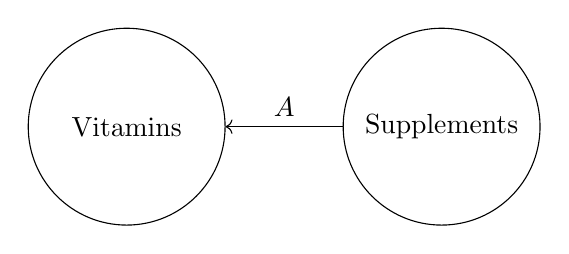
\begin{tikzpicture}
\node(S)[draw,circle,minimum size=2.5cm,inner sep=1pt] at (4,0) {Supplements};
\node(V)[draw,circle,minimum size=2.5cm,inner sep=1pt] at (0,0) {Vitamins};

\draw[->] (S) --node[above]{$A$} (V);

\end{tikzpicture}$$


Next, we record the relationship between days of the week and supplements:

$$B= \left( \begin{array}{rrr}
100 & 150\\
100 & 50\\
150 & 100
\end{array}\right)$$


Where now the rows are quantities of supplements and columns are days of the week.  So the 100 in the third row second column represents the 100mg taken on Wednesday of Supplement 3.  This to may be conceptualized as an arrow or transformation whose inputs are days of the week, and whose outputs are quantities of supplements.

$$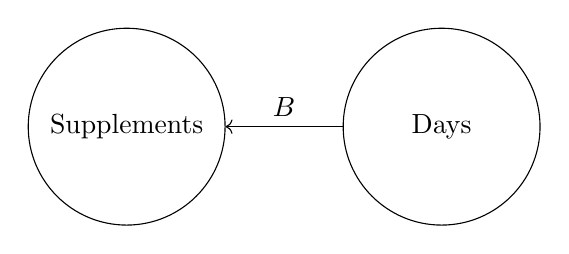
\begin{tikzpicture}
\node(S)[draw,circle,minimum size=2.5cm,inner sep=1pt] at (4,0) {Supplements};
%\node(V)[draw,circle,minimum size=2.5cm,inner sep=1pt] at (0,0) {Vitamins};
\node(D)[draw,circle,minimum size=2.5cm,inner sep=1pt] at (8,0) {Days};

%\draw[->] (S) --node[above]{A} (V);
\draw[->] (D) --node[above]{$B$} (S);

\end{tikzpicture}$$

Our goal now is to establish a relationship between days of the week and quantity of vitamins.

$$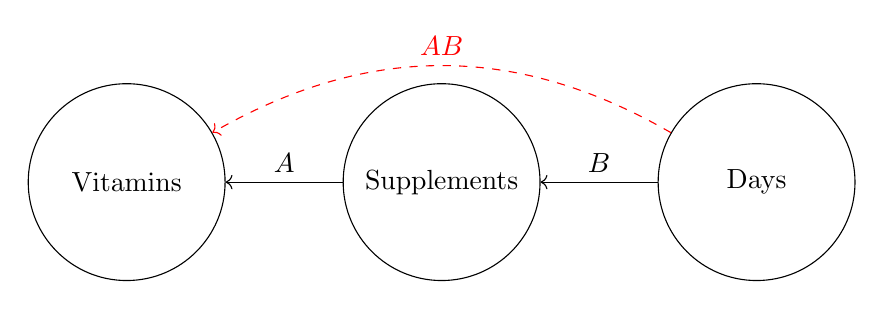
\begin{tikzpicture}
\node(S)[draw,circle,minimum size=2.5cm,inner sep=1pt] at (4,0) {Supplements};
\node(V)[draw,circle,minimum size=2.5cm,inner sep=1pt] at (0,0) {Vitamins};
\node(D)[draw,circle,minimum size=2.5cm,inner sep=1pt] at (8,0) {Days};

\draw[->] (S) --node[above]{$A$} (V);
\draw[->] (D) --node[above]{$B$} (S);

\draw [->, dashed, red] (D) to [out=150,in=30] node[above]{$AB$} (V);


\end{tikzpicture}$$

So, how much Vitamin A does Margo get on Monday?  She took \textcolor{blue}{100} mg of Supplement 1, of which \textcolor{red}{20\%} is Vitamin A, \textcolor{blue}{100} mg of Supplement 2, of which \textcolor{red}{10\%} is Vitamin A, and \textcolor{blue}{150} mg of Supplement 1, of which \textcolor{red}{50\%} is Vitamin A:

$$\left( \begin{array}{rrr}
\textcolor{red}{0.2} & \textcolor{red}{0.1} & \textcolor{red}{0.5}\\
0.2 & 0.3 & 0.1\\
0.2 & 0.4 & 0.2
\end{array}\right)\left( \begin{array}{rrr}
\textcolor{blue}{100} & 150\\
\textcolor{blue}{100} & 50\\
\textcolor{blue}{150} & 100
\end{array}\right)=\left( \begin{array}{cr}
\textcolor{red}{0.2}\cdot\textcolor{blue}{100}+\textcolor{red}{0.1}\cdot\textcolor{blue}{100}+\textcolor{red}{0.5}\cdot\textcolor{blue}{150} & ? \\
? & ? \\
? & ? 
\end{array}\right)=\left( \begin{array}{cr}
105 & ? \\
? & ? \\
? & ? 
\end{array}\right).$$

So on Monday, Margo got 105 mg of vitamin A.  What about the amount of vitamin D she received on Wednesday?  She took \textcolor{blue}{150} mg of Supplement 1, of which \textcolor{red}{20\%} is Vitamin D, \textcolor{blue}{50} mg of Supplement 2, of which \textcolor{red}{30\%} is Vitamin D, and \textcolor{blue}{100} mg of Supplement 1, of which \textcolor{red}{10\%} is Vitamin A:

\begin{eqnarray*}
\left( \begin{array}{rrr}
0.2 & 0.1 & 0.5\\
\textcolor{red}{0.2} & \textcolor{red}{0.3} & \textcolor{red}{0.1}\\
0.2 & 0.4 & 0.2
\end{array}\right)\left( \begin{array}{rrr}
100 & \textcolor{blue}{150}\\
100 & \textcolor{blue}{50}\\
150 & \textcolor{blue}{100}
\end{array}\right)&=&\left( \begin{array}{cr}
105 & ? \\
? & \textcolor{red}{0.2}\cdot\textcolor{blue}{150}+\textcolor{red}{0.3}\cdot\textcolor{blue}{50}+\textcolor{red}{0.1}\cdot\textcolor{blue}{100} \\
? & ? 
\end{array}\right)\\
&=&\left( \begin{array}{cr}
105 & ? \\
? & 55 \\
? & ? 
\end{array}\right).
\end{eqnarray*}

So Margo got 55 mg of Vitamin D on Wednesday.  Following this line of thinking, we obtain matrix:

$$\left( \begin{array}{rrr}
{0.2} & {0.1} & {0.5}\\
0.2 & 0.3 & 0.1\\
0.2 & 0.4 & 0.2
\end{array}\right)\left( \begin{array}{rrr}
{100} & 150\\
{100} & 50\\
{150} & 100
\end{array}\right)=\left( \begin{array}{cr}
105 & 85 \\
65 & 55 \\
90 & 70 
\end{array}\right).$$

This matrix records how much of each vitamin Margo had per day, where vitamins are rows and days are columns.  So on Monday, she got 90 mg of Vitamin E, and on Wednesday, she got 85 mg of Vitamin A.

\end{example}

So with this illustrative example in mind, we can define matrix multiplication.

\begin{definition}\label{Defn:MatrixProd}
For any matrix $M$, let $(M)_{ij}=m_{ij}$ denote the entry in the $i$th row and $j$th column.   Then, given a $m\times n$ matrix $A$ and a $n\times k$ matrix $B$, we define $AB$ the product of $A$ and $B$ to be a $m\times k$ matrix where:

$$(AB)_{ij}=\begin{pmatrix}\textcolor{red}{a_{i1}} & \textcolor{red}{a_{i2}} & \cdots & \textcolor{red}{a_{in}}\end{pmatrix}\begin{pmatrix}\textcolor{blue}{b_{1j}} \\ \textcolor{blue}{b_{2j}} \\ \vdots \\ \textcolor{blue}{b_{nj}}\end{pmatrix}=\begin{pmatrix}\textcolor{red}{a_{i1}}\textcolor{blue}{b_{1j}}+\textcolor{red}{a_{i2}}\textcolor{blue}{b_{2j}}+\cdots+\textcolor{red}{a_{in}}\textcolor{blue}{b_{nj}} \end{pmatrix}$$

\end{definition}

\textbf{Note that the number of columns of $A$ and the number of rows of $B$ must be the same.}  Recall Example \ref{Example:VitProd}, the outputs of $B$ corresponded to the rows, and the inputs of $A$ corresponded to it's columns, so these had to match up.  This number is also the $n$ is Definition \ref{Defn:MatrixProd}.


\begin{example}\label{Example:MoreMatrixProducts}
Let $$A=\begin{pmatrix}
1 & 2 & 3\\ 4 & 5 & 6
\end{pmatrix}, B=\begin{pmatrix}
0.2 & 0.4 \\ 0.5 & 0.6 \\ 0.1 & 0.8
\end{pmatrix}, C=\begin{pmatrix}
10 \\ 20 \\ 15
\end{pmatrix}.$$
Find:

\begin{enumerate}
    \item $AB$.
    \begin{eqnarray*}
    AB=\begin{pmatrix}
1 & 2 & 3\\ 4 & 5 & 6
\end{pmatrix}\begin{pmatrix}
0.2 & 0.4 \\ 0.5 & 0.6 \\ 0.1 & 0.8
\end{pmatrix}&=&\begin{pmatrix}
1\cdot0.2+2\cdot0.5+3\cdot0.1 & 1\cdot0.4+2\cdot0.6+3\cdot0.8\\
4\cdot0.2+5\cdot0.5+6\cdot0.1 & 4\cdot0.4+5\cdot0.6+6\cdot0.8 
\end{pmatrix}\\
&=&\begin{pmatrix}
1.5 & 4 \\ 3.9  &  9.4
\end{pmatrix}
    \end{eqnarray*}
    
    
    
    \item $BA$.
    \begin{eqnarray*}
    BA=\begin{pmatrix}
0.2 & 0.4 \\ 0.5 & 0.6 \\ 0.1 & 0.8
\end{pmatrix}\begin{pmatrix}
1 & 2 & 3\\ 4 & 5 & 6
\end{pmatrix}&=&\begin{pmatrix}
0.2\cdot1+ 0.4\cdot 4 & 0.2\cdot2+ 0.4\cdot 5 & 0.2\cdot3+ 0.4\cdot6\\
0.5\cdot1+ 0.6\cdot 4 & 0.5\cdot2+ 0.6\cdot 5 & 0.5\cdot3+ 0.6\cdot6\\
0.1\cdot1+ 0.8\cdot 4 & 0.1\cdot2+ 0.8\cdot 5 & 0.1\cdot3+ 0.8\cdot6\\
\end{pmatrix}\\
&=&\begin{pmatrix}
1.8 & 2.4 & 3 \\ 2.9  &  4 & 5.1 \\ 3.3 & 4.2 & 5.1
\end{pmatrix}
    \end{eqnarray*}    
    
    \item $AC$.
    \begin{eqnarray*}
    AC=\begin{pmatrix}
1 & 2 & 3\\ 4 & 5 & 6
\end{pmatrix}\begin{pmatrix}
10\\20\\15
\end{pmatrix}&=&\begin{pmatrix}
1\cdot10+2\cdot20+3\cdot15 \\ 4\cdot10+5\cdot20+6\cdot15
\end{pmatrix}\\
&=&\begin{pmatrix}
95 \\ 230
\end{pmatrix}
    \end{eqnarray*}
    
    
    
    \item $CA$.
    
    Notice that if we try to take the product $CA$:
    \begin{eqnarray*}
    CA=\begin{pmatrix}
10\\20\\15
\end{pmatrix}\begin{pmatrix}
1 & 2 & 3\\ 4 & 5 & 6
\end{pmatrix}&=&\begin{pmatrix}
10\cdot1+?\cdot4 & 10\cdot2+?\cdot5 & 10\cdot3+?\cdot6 \\ 20\cdot1+?\cdot4 & 20\cdot2+?\cdot5 & 20\cdot3+?\cdot6\\15\cdot1+?\cdot4 & 15\cdot2+?\cdot5 & 15\cdot3+?\cdot6
\end{pmatrix}
    \end{eqnarray*}
Since the number of columns of the first matrix do not match with the number of rows of the second matrix, the product is not defined.    
    
    \item $BC$.
    
    Since $B$ has 2 columns and $C$ has 3 rows, these values do not match and this product is not defined.
    \item $CB$.
    
    Since $C$ has 1 column and $B$ has 2 rows, these values do not match and this product is not defined.
\end{enumerate}


\end{example}

Something we should observe here is that, unlike products of real numbers, products of matrices are \textbf{NOT} commutative.  In Example \ref{Example:MoreMatrixProducts}, $AB\neq BA$, and $AC$ was defined whereas $CA$ was not.

Another way matrix products deviate from real number products is that the product of matrices whose entries aren't 0 can result in a matrix whose entries are all 0.

\begin{example}
Let $$A=\begin{pmatrix}1&2\\2&4 \end{pmatrix}, B=\begin{pmatrix}2&6\\-1&-3 \end{pmatrix}.$$

Notice that:

\begin{eqnarray*}
AB=\begin{pmatrix}1&2\\2&4 \end{pmatrix}\begin{pmatrix}2&6\\-1&-3 \end{pmatrix}&=&\begin{pmatrix}
1\cdot 2+2\cdot(-1) & 1\cdot 6+2\cdot(-3)\\ 2\cdot 2+4\cdot(-1)&2\cdot 6 +4\cdot(-3)
\end{pmatrix}\\
&=&\begin{pmatrix}
0 & 0 \\ 0 & 0
\end{pmatrix}.
\end{eqnarray*}
Although neither $A$ nor $B$ have 0 entries, their product is an all 0 matrix.  Also notice that this does not mean $BA$ is an all 0 matrix.

\begin{eqnarray*}
BA=\begin{pmatrix}2&6\\-1&-3 \end{pmatrix}\begin{pmatrix}1&2\\2&4 \end{pmatrix}&=&\begin{pmatrix}
2\cdot 1+6\cdot2 & 2\cdot 2+6\cdot4\\ (-1)\cdot 1+(-3)\cdot2&(-1)\cdot 2 +(-3)\cdot4
\end{pmatrix}\\
&=&\begin{pmatrix}
14 & 28 \\ -7 & -14
\end{pmatrix}.
\end{eqnarray*}

\end{example}






\subsection{Sums of Matrices}

Matrix sums are much more straight forward than their products.  Two Matrices need to have the same dimensions in order to be summed, and the sum is just the sum of the entries, so:

$$\begin{pmatrix} a & b \\ c & d \end{pmatrix}+ \begin{pmatrix} w & x \\ y & z \end{pmatrix}=\begin{pmatrix} a+w & b+x \\ c+y & d+z \end{pmatrix}$$


\begin{example}
Company $B$ gets in on this action and will give 2 dollars to each charity for each student who attends.  NOW given $F$ female and $M$ male students, how much money will go to Elderly and the Homeless?

\begin{eqnarray*}
\begin{pmatrix} 0.8 & 0.5 & 0 \\ 0.2 & 0.5 & 1 \end{pmatrix} \left( \begin{pmatrix} 2 & 1 \\ 1 & 2 \\ 2 & 2\end{pmatrix} + \begin{pmatrix} 2 & 2 \\ 2 & 2 \\ 2 & 2\end{pmatrix}   \right)\begin{pmatrix} F\\M \end{pmatrix}&=&\begin{pmatrix} 0.8 & 0.5 & 0 \\ 0.2 & 0.5 & 1 \end{pmatrix} \begin{pmatrix} 4 & 3 \\ 3 & 4 \\ 4 & 4\end{pmatrix} \begin{pmatrix} F\\M \end{pmatrix}\\
&=&\begin{pmatrix} 4.7 & 4.4 \\ 7.3 &  6.6 \end{pmatrix}\begin{pmatrix} F\\M \end{pmatrix}\\
&=&\begin{pmatrix} 4.7F+4.4M\\ 7.3F+6.6M \end{pmatrix}\\
\end{eqnarray*}
So \$$4.7 F+4.4M$ for Elderly and $\$7.3 F+6.6M$ for Homeless.
\end{example}

\section{Computation using Sage}

As usual, this seems like it should be much easier using technology.  Let's suppose $A=\begin{pmatrix} 1 & 2 \\ 3 & 4\end{pmatrix}, B=\begin{pmatrix} 5 & 6 \\ 7 & 8\end{pmatrix}$.  Verify that:

\begin{eqnarray*}
A+B&=&\begin{pmatrix} 6 & 8 \\ 10 & 12\end{pmatrix}\\
AB&=&\begin{pmatrix} 19 & 22 \\ 43 & 50\end{pmatrix}\\
BA&=&\begin{pmatrix} 23 & 34 \\ 31 & 46\end{pmatrix}
\end{eqnarray*}


\url{https://sagecell.sagemath.org/?z=eJxztM1NLCnKrNAIDNRRiI421DGK1Yk21jGJjdXk5XJClTTVMQNKmutYgCULijLzSjQctZ0QbC0E20nLURMAu6IZgA==&lang=sage}



\chapter{Linear Programming}\label{Chapter:LinearProgramming}


\section{Linear Inequalities}\label{Section:LinearInequalities}

Remember when we said the solution to something like $$2x+3y=12$$ is the collection of all points $(x,y)$ that make this statement true.  For equations of the form above, that forms a line.  If however if we replace the $=$ with an inequality like so:

$$2x+3y\leq12$$

What we now mean is every pair $(x,y)$ that make THIS statement true.  So that would include every point on the line $2x+3y=12$, as well as say $(0,0), (1,2), (1,3)$ but not $(1,4)$ (plug them in to see why.)  Obviously, just like in lines, we don't want to test every one of infinitely many points to see what's going on.\\

So, we note that $2x+3y=12$ is a line:  \url{https://www.desmos.com/calculator/spsryp8xxl}

The inequality $2x+3y\leq12$ is not just this line, but the entire half of the plane where $2x+3y$ is some value that is less than 12.  The number 12 cuts the number line in half, numbers less than, and greater than 12, so it makes sense that this line cuts the $x,y$ plane in half as well, we just need to pick a half.\\

Well, we know that $2(0)+3(0)=0\leq12$, and so our half should be the half that contains $(0,0)$.  In general, you can pick any point you want and test it.  For example, if we picked (5,5), we would observe that $2(5)+3(5)=25\not\leq 12$ and so we should pick the half that DOESN'T contain $(5,5)$.  Either way, we obtain: \url{https://www.desmos.com/calculator/yvb1odxncf}


\section{Systems of Linear Inequalities}\label{Section:SystemsLinearInequalities}

If a solution to a system of equations is a set of points that make several equations true, then the same is true of systems of linear inequalities.  It's just going to be the collection of points that make all the inequalities true.


\begin{example}
What is the solution to the following system:

\begin{eqnarray*}
2x+3y&\leq&12\\
x&\geq&0\\
y&\geq&0
\end{eqnarray*}

We know from earlier that the solutions have to lie in the bottom right hand of the plane on or below the line $2x+3y=12$.  We also know that neither the $x$ or $y$ values can be negative.  What's left is a sort of triangle: \url{https://www.desmos.com/calculator/2dekmagipa}, the overlap of regions where all 3 inequalities are true.\\

This may be easier to see: \url{https://www.desmos.com/calculator/apmcey4kfa}.





\end{example}

\newpage
\section{Linear Optimization}\label{Section:LinearOptimization}

\begin{example}
Find $(x,y)$ such that:

\begin{eqnarray*}
2x+3y&\leq&12\\
x&\geq&0\\
y&\geq&0
\end{eqnarray*}

and $f(x,y)=x+y$ is maximized.\\

From above, we know that this region is a triangle in the first quadrant.  We want to find the point(s) in this region where by taking the sum of the points, we get as large as a value as possible.  There are infinitely many points in this region, how are we ever going to find the one that makes this sum the largest?\\

Well, we know that given every possible output from the objective function $f$ i.e.\ every possible $k$ so that $x+y=k$, this actually defines a line: \url{https://www.desmos.com/calculator/qststwgxro}.  In the link you can see the line when $k=0$.  There is one point $(0,0)$ which is actually a part of our region which would give this output.  As we drag $k$ upwards, we see that there is a line segment worth of points in our region which would give that $k$ as an output.  At $k=4$ \url{https://www.desmos.com/calculator/iy5rq5hpxa} we hit a corner of the region but we see that we can still increase $k$.  Now at $k=6$ \url{https://www.desmos.com/calculator/qwrti1mxln}, we see that we've hit another corner.  Very importantly, if we try to increase $k$ at all, our line will fall outside of the feasible region and there will be no points that would give such a $k$ as an output.\\

So, it must be that the largest $k$ can be is 6, and that this happens at $(6,0)$.  One can check to see that this point satisfies all the criteria above.  Most importantly though: \textbf{IT MEANS TO FIND OPTIMAL SOLUTIONS ONE JUST NEEDS TO FIND THE CORNERS OF THE REGION}.  This is because if your line isn't on a corner, you can still slide that value up or down, so the corresponding $k$ value is neither maximal or minimal.


\end{example}

\begin{example}

Suppose that a agriculture student is raising goats and pigs for a project.  The goal is to raise some animals and then sell them for profit.  She can raise a total of at most 16 animals.  It costs \$25 per goat and \$ 75 per pig, and she has a budget of \$900.  Finally, she doesn't particularly like goats, so she won't raise more than 10 of them.  If the profit per goat is \$12 and profit per pig is \$40, how many of each should she raise to maximize profits?\\

We should note, if $x$ is the number of goats and $y$ the number of pigs, then she is maximizing $P(x,y)=12x+40y$.  The inequalities she is dealing with are:

\begin{eqnarray*}
x+y&\leq&16\ \ \text{at most 16 animals}\\
25x+75y&\leq&900\ \ \text{\$900 budget}\\
x&\leq&10\ \ \text{hates goats}\\
x&\geq&0\ \ \text{no negative goats}\\
y&\geq&0\ \ \text{no negative pigs}
\end{eqnarray*}

Sketching our region out we get:  \url{https://www.desmos.com/calculator/lwbkvibuyq}, with corner points:

$$\begin{array}{c|c|c}
x & y & P(x,y)\\
\hline
0 & 0 & 12(0)+40(0)=0\\
10 & 0 & 12(10)+40(0)=120\\
10 & 6 & 12(10)+40(6)=360\\
6 & 10 & 12(6)+40(10)=472\\
0 & 12 & 12(0)+40(12)=480\\
\end{array}$$

So the profit is maximized when you raise 12 pigs and no goats.  To get a better sense of how we found these corners, these are just system of $2\times 2$ systems of equations: \url{https://www.desmos.com/calculator/bzczxrkggy}


\end{example}










\chapter{Logic}\label{Chapter:Logic}


\section{Statements}\label{Section:Statements}

Something thats often misunderstood about Math is that people think that Math is the study of numbers.  This is false, and not even historically justifiable.  Certainly numeracy has taken on a great role within mathematics, but that is not fundamentally what the discipline is.  Really, even when Math deals with numbers, the fundamental thing that is studied are not numbers but \textbf{statements}.  What is a statement?  It is a sentence that is true or false, but not both.  For example:

\begin{enumerate}
\item MSU-Billings is a State School.
\item $10+5=12$.
\item $x<4$.
\end{enumerate}

The first sentence is a true sentence, the second sentence is a false sentence.  The third is true or false depending on the value of $x$, but at no point can it take on the value of both true and false.\\

So we're going to be doing something in this chapter that seems fairly strange. We are going to be working with variables that are placeholders for statements rather than numbers.  The possible values for these statements then, are ``True" and ``False".  We will be performing operations on these statements as in standard algebra, but since every variable has only 2 possible values, the rules of our algebra are going to be different.


\section{Operations on Statements}\label{Section:OperationsStatements}

\subsection{Not}

The first sort of operation we can perform is  \textbf{negation}.  Given any statement, the negation is a statement that is false whenever the original statement is true, and true when the original is false.\\

For example if $p=\text{``It will rain today"}$,  then it's negation $\sim p=\text{``it will not rain today"}$, similarly if $q=``x>10"$, then it's negation $\sim q =``x\leq 10"$.  These are statements that are true whenever the original statement is false and false when they are true.\\

A convenient way to record when a statement is true or false is by something called a ``truth table".  By listing all the truth values of $p$, we can see when $\sim p$ is true:

$$\begin{array}{c|c}
p&\sim p\\
\hline
T & F\\
F&T
\end{array}$$


\subsection{And}

Given statements $p$, $q$, the statement $p\wedge q$ pronounced $p$ and $q$ is when $p$ and $q$ are both true, otherwise it is false.\\

For example, if $p=$``I will eat breakfast today" and $q=$``I will eat lunch today", then the statement $p\wedge q$ is the statement ``I will breakfast today and I will eat lunch today" which is only true if you eat both meals, if you skip one or both, then it is false.

$$\begin{array}{c|c|c}
p&q&p\wedge q\\
\hline
T & T&T\\
T&F&F\\
F&T&F\\
F&F&F
\end{array}$$

So if you skipped breakfast but had lunch, you could take a look at the third line and see that the compound statement ``I will breakfast today and I will eat lunch today" is false.



\subsection{Or}

Given statements $p$, $q$, the statement $p\vee q$ pronounced $p$ or $q$ is when either $p$ or $q$ is true, otherwise it is false.\\

So as in the above example, $p\vee q$ would be ``I will eat breakfast today or I will eat lunch today" and you're covered as long as you either have breakfast or lunch.  If you skip both, then you're lying, but as long as you had either you're telling the truth.

$$\begin{array}{c|c|c}
p&q&p\vee q\\
\hline
T & T&T\\
T&F&T\\
F&T&T\\
F&F&F
\end{array}$$

So if you had breakfast and skipped lunch, you can look at the second row and see that the statement ``I will eat breakfast today or I will eat lunch today" is still true.


\section{Compound Statements}\label{Section:CompoundStatements}

Suppose a friend of your has a test coming up tomorrow .  You ask them about their study plans and they say ``Well, I'll either study today, or I'll skip class tomorrow and study tomorrow."  Now your friend says this, but all sorts of things could happen between now and the test, so under what circumstances is your friend telling the truth and when are they lying?\\

Looking at their statement, there seems to be three fundamental underlying events:

\begin{itemize}
\item Studying today, lets call this $p$.
\item Going to class tomorrow, let's call this $q$.
\item Studying tomorrow, let's call this $r$.
\end{itemize}

Then the sentence ``I'll either study today, or I'll skip class tomorrow and study tomorrow." can be broken down as: $$p\vee (\sim q \wedge r)$$ that is ``Either $p$ OR not $q$ AND $r$".  \\

So when is this statement true?  We first note that $p,q,r$ could all be true or false, your friend could potentially do or not do any of these things.  All the combinations are as follows:

 $$\begin{array}{c|c|c}
p&q&r\\
\hline
T & T&T\\
T&T&F\\
T&F&T\\
T&F&F\\
F & T&T\\
F&T&F\\
F&F&T\\
F&F&F
\end{array}$$

Since $\sim q$ is in our expression, it may be helpful to list out what it's values are.  Remember, that $\sim q$ is the opposite of $q$.  As you get more experienced one may be tempted to skip stuff like $\sim q$ but for now let's proceed with caution:

 $$\begin{array}{c|c|c|c}
p&q&r&\sim q\\
\hline
T & T&T&F\\
T&T&F&F\\
T&F&T&T\\
T&F&F&T\\
F & T&T&F\\
F&T&F&F\\
F&F&T&T\\
F&F&F&T
\end{array}$$

Next, we have the statement $\sim q \wedge r$, which is true whenever both $\sim q$ and $r$ are true\ldots

 $$\begin{array}{c|c|c|c|c}
p&q&r&\sim q & \sim q \wedge r\\
\hline
T & T&T&F & \\
T&T&F&F& \\
T&F&\textcolor{red}{T}&\textcolor{red}{T}&\textcolor{red}{T}\\
T&F&F&T\\
F & T&T&F\\
F&T&F&F\\
F&F&\textcolor{red}{T}&\textcolor{red}{T}&\textcolor{red}{T}\\
F&F&F&T
\end{array}$$

\ldots and false otherwise:

 $$\begin{array}{c|c|c|c|c}
p&q&r&\sim q & \sim q \wedge r\\
\hline
T & T&T&F&F\\
T&T&F&F&F \\
T&F&T&T&T\\
T&F&F&T&F\\
F & T&T&F&F\\
F&T&F&F&F\\
F&F&T&T&T\\
F&F&F&T&F
\end{array}$$

Finally, we have the statement $p\vee (\sim q \wedge r)$ which is true whenever either $p$ or $\sim q \wedge r$ is true \ldots


 $$\begin{array}{c|c|c|c|c|c}
p&q&r&\sim q & \sim q \wedge r& p\vee(\sim q \wedge r)\\
\hline
\textcolor{red}{T} & T&T&F&F&\textcolor{red}{T}\\
\textcolor{red}{T}&T&F&F&F&\textcolor{red}{T} \\
\textcolor{red}{T}&F&T&T&\textcolor{red}{T}&\textcolor{red}{T}\\
\textcolor{red}{T}&F&F&T&F&\textcolor{red}{T}\\
F & T&T&F&F\\
F&T&F&F&F\\
F&F&T&T&\textcolor{red}{T}&\textcolor{red}{T}\\
F&F&F&T&F
\end{array}$$

\ldots and false otherwise:


 $$\begin{array}{c|c|c|c|c|c}
p&q&r&\sim q & \sim q \wedge r& p\vee (\sim q \wedge r)\\
\hline
T & T&T&F&F&T\\
T&T&F&F&F&T \\
T&F&T&T&T&T\\
T&F&F&T&F&T\\
F & T&T&F&F&F\\
F&T&F&F&F&F\\
F&F&T&T&T&T\\
F&F&F&T&F&F
\end{array}$$

If your friend studies today, goes to class tomorrow and studies tomorrow, did they lie?  In this case $p$ is true, $q$ is true and $r$ is true, so looking at the first row:

 $$\begin{array}{c|c|c|c|c|c}
p&q&r&\sim q & \sim q \wedge r& p\vee (\sim q \wedge r)\\
\hline
\textcolor{blue}{T} & \textcolor{blue}T&\textcolor{blue}T&F&F&\textcolor{blue}T\\
T&T&F&F&F&T \\
T&F&T&T&T&T\\
T&F&F&T&F&T\\
F & T&T&F&F&F\\
F&T&F&F&F&F\\
F&F&T&T&T&T\\
F&F&F&T&F&F
\end{array}$$

Your friend was telling the truth!  Let's say instead, they didn't study today, went to class tomorrow and studied tomorrow.  Then $p$ is false, $q$ is true, $r$ is true and we have:

 $$\begin{array}{c|c|c|c|c|c}
p&q&r&\sim q & \sim q \wedge r& p\vee (\sim q \wedge r)\\
\hline
T & T&T&F&F&T\\
T&T&F&F&F&T \\
T&F&T&T&T&T\\
T&F&F&T&F&T\\
\textcolor{blue}F & \textcolor{blue}T&\textcolor{blue}T&F&F&\textcolor{blue}F\\
F&T&F&F&F&F\\
F&F&T&T&T&T\\
F&F&F&T&F&F
\end{array}$$

Then, they would be lying.  They said either they would go to class today (they didn't) or, they would skip class AND study tomorrow.  They studied tomorrow but didn't skip class, so what they said ultimately wasn't true.






\subsection{Sage}

We can automatically generate the truth tables with SageCells.  Using the symbols:

\begin{itemize}
\item    $\&$ -and
\item    $|$-or
\item    $\sim$-not
\item    $\wedge$-xor
 \item   $->$-if-then
\item    $<->$-if and only if
\end{itemize}


We haven't covered all these operations yet.  But if we wanted to say ``$p$ or (not $q$ and $r$)"  That could be recorded as $p|(\sim q\&r)$.  So we could generate the truth table here:  \url{https://sagecell.sagemath.org/?z=eJxLU7BVKCjKL0hOzEnWS8svyi3NSdRQKqjRqCtUK9JU0uTlStMrKSotyShJTMpJ1dAEAIzpD_A=&lang=sage}  It generates the table in a different order than what we have but the same rows still correspond to the same values.



\section{Equivalent Statements}\label{Section:EquivalentStatements}


Naturally, in mathematics, we care about equivalence of things.  For example, one might say that given any $x$, $2(x+3)=2x+6$.  Another example of equivalent statements would be ``I own a red dog" and ``I own a dog and it is red."  Suffice to say, the same information can be transmitted in a lot of distinct ways, and we should have some mechanism for detecting that.\\

Let's take a closer look at $2(x+3)=2x+6$.  What does this really mean?  In essence, it says that no matter what $x$ is, the left hand side and right hand side will yield the same value.  If I plug in $x=0$ then $2(0+3)=2(0)+6=6$, if I plug in $x=4$ then $2(4+3)=2(4)+6=14$, if I plug in $x=-1$ then $2(-1+3)=2(-1)+6=4$ and so forth.  The statements $2(x+3)$ and $2x+6$ have the same value under the same circumstances.  So this is how we define equivalence of logical statements. \textbf{Two logical statements are equivalent if they have the same values under the same circumstances.}\\

For algebraic expressions like the ones above, $x$ can take on infinitely many values, so we can't just sit there and plug in infinitely many values into both sides, so it becomes imperative that we establish some sort of general rules and laws, like distribution, to avoid having to do this, while still being able to meaningfully accomplish things.  The nice thing about logical statements is that for any variable, we only have 2 possible values, $T$ or $F$.  The statement itself can only take on the values $T$ or $F$, so it's much easier to see if two logical statements are equivalent, compared to algebraic ones.\\

\begin{example}
Is ``$\sim(p \vee q)=\sim p \vee \sim q$?"\\

Before we jump into the formal stuff, it helps to concretize this with actual statements.  Let's say $p$ is ``I'll eat breakfast" and $q$ is ``I'll eat lunch".  Then $p \vee q$ is ``I'll eat breakfast or I'll eat lunch".  Is NOT doing this the same as $\sim p \vee \sim q$ which is ``I'll not eat breakfast or I'll not eat lunch?"\\

The first statement is basically ``I'm not eating breakfast or lunch", the second is ``I'll not eat breakfast or I'll not eat lunch", they sound similar spoken aloud but there is a subtle difference.\\

Let's say you skip breakfast and eat lunch.  Since you ate lunch, $p\vee q$ is true, so $\sim(p\vee q)$ must be false, you didn't not eat breakfast or eat lunch.  What about $\sim p \vee \sim q$?  Well you skipped breakfast so $\sim p$ is true and therefore $\sim p \vee \sim q$ is true, so it would seem like they are not the same.\\

Formally, we can look at these truth tables:

$$\begin{array}{c|c|c|c}
p&q&p\vee q& \sim (p\vee q)\\
\hline
T & T&T&F\\
T&F&T&F\\
F&T&T&F\\
F&F&F&T
\end{array}$$

$$\begin{array}{c|c|c|c|c}
p&q&\sim p& \sim q & \sim p \vee \sim q\\
\hline
T & T&F&F&F\\
T&F&F&T&T\\
F&T&T&F&T\\
F&F&T&T&T
\end{array}$$

So $\sim(p\vee q)$ i.e.\ ``I'm not eating breakfast or lunch" is only true if you skip both meals.  If you eat either then you lied.  On the other hand, $\sim p \vee \sim q$ i.e.\  ``I'll skip breakfast or I'll skip lunch" is true so long as you skip either meal.  It's only false if you go ahead and eat both.\\

So what does $\sim(p \vee q)$ equal?
\end{example}

\begin{example}
Does $\sim(p \vee q)=\sim p \wedge \sim q$?\\

Start with the concrete before the formal.  In our extended example, $\sim(p\vee q)$ means ``I'm not eating breakfast or lunch", whereas $\sim p \wedge \sim q$ means ``I'm not eating breakfast and I'm not eating lunch."  It does kinda seem like they're the same\ldots\\

So formally:

$$\begin{array}{c|c|c|c}
p&q&p\vee q& \sim (p\vee q)\\
\hline
T & T&T&F\\
T&F&T&F\\
F&T&T&F\\
F&F&F&T
\end{array}$$

$$\begin{array}{c|c|c|c|c}
p&q&\sim p& \sim q & \sim p \wedge \sim q\\
\hline
T & T&F&F&F\\
T&F&F&T&F\\
F&T&T&F&F\\
F&F&T&T&T
\end{array}$$

now THIS makes more sense.  In order to say ``I'm not having breakfast OR lunch"  you really are saying ``I'm skipping breakfast AND I'm skipping lunch".  So these statements are in fact identical, they have the same values under the same circumstances.\\

This is half of a pair of equivalences called \textbf{DeMorgan's Laws}:

\begin{itemize}
\item $\sim(p \vee q)=\sim p \wedge \sim q$
\item $\sim(p \wedge q)=\sim p \vee \sim q$
\end{itemize}

It's not a bad idea to check this second equivalence, build the truth tables and see if they are the same.

\end{example}



\begin{example}
Is $\sim((p \vee q)\wedge \sim r)=(\sim p \wedge \sim q )\vee r$?\\

So yeah sure, we could go ahead and build truth tables for all this, but at this point Im sure laying out 8 rows of T and F and all these combinations is a real hassle.  On the other hand, we have in fact these very nice laws described above.  One of the reasons we develop algebraic rules is convenience, so let's go ahead:

\begin{eqnarray*}
\sim((p \vee q)\wedge \sim r)&=&\sim(p \vee q)\vee \sim\sim r\ \ \text{By DeMorgan's Law}\\
&=&\sim(p \vee q)\vee r \ \ \text{since $\sim\sim r=r$}\\
&=&(\sim p \wedge \sim q )\vee r \ \ \text{by DeMorgans law again.}
\end{eqnarray*}

So yes, they are equal, fairly nice.
\end{example}



\section{Conditional Statements}\label{Section:ConditionalStatements}

These things go by a few names, conditional statements, if-then statements.  They are statements of the form ``If $p$, then $q$."  When the condition $p$ is satisfied, it implies the statement $q$.  This is written in formal logic as $p\to q.$\\


Let's suppose that you have a child and you say to them ``If you are clean your room, I'll buy you ice-cream!"  What would make you a liar and what would make you a truth teller.\\

If your kid cleans their room, and you buy them ice-cream, then hooray, you kept your promise!  If your kid cleans their room and and you don't buy them ice-cream, then you didn't keep your promise and are a liar.\\

Now this part is sometimes tricky for students, but bear with me.  If your kid doesn't clean their room, you can do whatever you want.  You only said that you would do something if they cleaned their room, you made no promises as to what you would do if they didn't.  So now whether or not you buy them ice-cream, you've technically kept your promise.  This may make you a pushover parent, depending, but it wouldn't make you a liar.\\

So, if we let $p$=``kid cleans room" and $q$=``you buy them ice-cream"  Then the above sentence may be written as $p\to q$ which has the following truth table:

$$
\begin{array}{c|c|c}
p&q&p\to q\\
\hline
T&T&T\\
T&F&F\\
F&T&T\\
F&F&T
\end{array}
$$


As we can see ``If $p$ then $q$" is always true unless $p$ happens and then $q$ does not happen as promised.

\subsection{An equivalent statement}

Notice that $p\to q$ is only false under one circumstance.  So is the statement $p\vee q$.  Is it possible then to rewrite $p\to q$ as an ``or" statement somehow?\\

I claim that $p \to q = \sim p \vee q$.  To see this, consider:


 
$$
\begin{array}{c|c|c|c|c}
p&q&p\to q&\sim p & \sim p \vee q\\
\hline
T&T&T&F&T\\
T&F&F&F&F\\
F&T&T&T&T\\
F&F&T&T&T
\end{array}
$$

And we see that these things have the same truth values and are equivalent statements.  But, more importantly, consider what $\sim p \vee q$ would mean in our example.  ``Either you don't clean your room or you can have ice-cream."  One might rephrase this as ``You can either not clean your room or you can have ice-cream."  Isn't this basically saying ``If you clean your room you can have ice-cream?"  So that definitely sounds like an equivalent statement to me.

\subsection{Negation}

What about the negation of $p\to q$?  Well, one can try all sorts of combinations of $p, q$, but what we do know is how to negate and/or statements, and how to rewrite $p\to q$ so:

\begin{eqnarray*}
\sim(p\to q)&=&\sim(\sim p \vee q)\\
&=&\sim\sim p\wedge \sim q\\
&=&p\wedge \sim q.
\end{eqnarray*}

How does that play out in practice, again using our parenting example, $p\wedge \sim q$ is ``You cleaned your room and I'm not buying you ice-cream."  Damn.  That's basically exactly the opposite of what you said before, which is what a negation is supposed to be.  

\subsection{A Longer Example}

Using these facts, we can take relatively complicated statements, break them down, and negate them with relative ease.  Consider this sentence:\\

``If it is sunny and I am in a good mood, then I will take a walk."\\

So let's let:

\begin{itemize}
\item $p$=``It's Sunny"
\item $q$=``I'm in a good mood."
\item $r$=``I take a walk".
\end{itemize}

We can summarize this whole thing as $(p\wedge q)\to r$.  It's not the easiest thing to see when this statement may be true.  So, we can break this thing down as follows:

\begin{eqnarray*}
(p\wedge q)\to r&=&\sim (p\wedge q)\vee r\\
&=&(\sim p \vee \sim q) \vee r
\end{eqnarray*}

So this is an equivalent statement, and it's not much easier to see that it is true as long as it isn't sunny, you're in a bad mood, or if you take a walk. We would read this as ``Either it's not sunny, or I'm not in a good mood, or I'm taking a walk." \\ 

 If we negate this thing:



\begin{eqnarray*}
\sim ((p\wedge q)\to r)&=&\sim ((\sim p \vee \sim q) \vee r)\\
&=&\sim (\sim p \vee \sim q) \wedge \sim r\\
&=& (\sim \sim p  \wedge \sim \sim q) \wedge \sim r\\
&=&(p\wedge q)\wedge \sim r
\end{eqnarray*}

We would read this as ``It IS sunny and I'm in a good mood and for some reason I'm not going to walk." which is the opposite of what was promised before.


\subsection{Misconceptions}

There are some common misinterpretations of the conditional statement that should be addressed.  In particular, there are colloquial statements which people believe that are equivalent to the conditional which are not.\\

Given the statement $p\to q$, is it equivalent to say $q\to p$?  (We say that $q\to p$ is the \textbf{converse} of $p\to q$.)  We can check with truth tables, but before that, let's ask ourselves this:  Suppose that $p=$``I drink bleach" and $q=$``I get sick."  I think we can all buy that $p\to q$ i.e.\ if I drink bleach then I will get sick.  Now the converse, $q\to p$ is the statement ``If I get sick, then I drank bleach".  Is this the same statement?\\

Doesn't seem so, you could have gotten sick from any sort of things, it didn't have to be bleach.  Another example is if $p=$``I'm a square" and $q=$``I'm a rectangle."  All squares are rectangles, not all rectangles are squares.  So if $p\to q$, we can think of that as all the circumstances where $p$ is true lives inside the collection of circumstances where $q$ is true, and that the reverse is not the same thing.  And of course:

$$\begin{array}{c|c|c|c}
p & q & p\to q & q\to p\\
\hline
T & T & T & T\\
T & F & F & T\\
F & T & T & F \\
F & F & T & T
\end{array}$$


So these columns are not the same and so the statements are not equal.\\

What about $\sim p \to \sim q$? (This is the  \textbf{inverse} of $p\to q$)  Well this would be ``If I'm not drinking bleach then I won't get sick" or ``If I'm not a square then I'm not a rectangle."  This doesn't seem like it's true either.  You can not drink bleach, but then drink paint thinner instead and you'd be sick, and of course there are plenty of rectangles that aren't squares.  That and:

$$\begin{array}{c|c|c|c|c|c}
p & q & p\to q &\sim p & \sim q& \sim p\to \sim q\\
\hline
T & T & T & F & F & T\\
T & F & F & F & T &T\\
F & T & T & T & F & F \\
F & F & T & T & T & T
\end{array}$$


What about $\sim q \to \sim p$ (the \textbf{ contrapositive"} of $p\to q$)?  In our example, that would be, ``If I didn't get sick then I didn't drink bleach" or ``If I'm not a rectangle then I'm not a square".  These DO seem true.  If you didn't get sick you couldn't have drank bleach, if you're not a rectangle, there's no way you could be a square.  Rather than use truth tables, consider:

\begin{eqnarray*}
\sim q \to \sim p&=&(\sim \sim q \vee \sim p)\\
&=&q \vee \sim p\\
&=&\sim p \vee q\\
&=&p\to q.
\end{eqnarray*}

So these things ARE the same.


\subsection{Biconditional}

Maybe you want to describe 2 statements where $p\to q$ and $q\to p$, i.e. whenever 1 is true then the other is true.  Well this is literally $(p\to q)\wedge (q\to p)$.



$$\begin{array}{c|c|c|c|c}
p & q & p\to q & q\to p& (p\to q)\wedge (q\to p)\\
\hline
T & T & T & T&T\\
T & F & F & T&F\\
F & T & T & F &F\\
F & F & T & T&T
\end{array}$$



We symbolize this with $p\leftrightarrow q:$



$$\begin{array}{c|c|c}
p & q & p\leftrightarrow q \\
\hline
T & T & T \\
T & F & F\\
F & T & F \\
F & F & T 
\end{array}$$



\section{Circuits}\label{Section:Circuits}

Consider $$\begin{circuitikz}

\draw (0,0) to[ospst=$p$] (2,0);

\end{circuitikz}$$

This is the diagram of the ``circuit" $p$ Imagine $T$ as been the bridge open and $F$ as the bridge closed.  Can you cross over, well, yes as long as the bridge is open, i.e. as long as $p$ is true.\\

Now how about this:


Consider $$\begin{circuitikz}

\draw (0,0) to[ospst=$p$] (2,0);

\draw (2,0) to[ospst=$q$] (4,0);

\end{circuitikz}$$

Can you get to the other side?  Well, as long as both bridges are open, i.e.  $p\wedge q$.\\


How about this? $$\begin{circuitikz}

\draw (0,0) to (2,0);
\draw (2,0) to (2,1);
\draw (2,0) to (2,-1);

\draw (2,1) to[ospst=$p$] (4,1);

\draw (2,-1) to[ospst=$q$] (4,-1);

\draw(4,1) to (4,0);
\draw(4,-1) to (4,0);

\draw(4,0) to (6,0);


\end{circuitikz}$$


Can you get from one side to the other?  Yes, as long as either bridge is open we can, so this is $p\vee q$.\\

Using these circuit diagrams, we can model any logical statement.  For example $p\wedge ((q\wedge r) \vee (\sim q \wedge \sim r))$ would be:


$$\begin{circuitikz}

\draw (0,0) to[ospst=$p$] (2,0);
\draw (2,0) to (2,1);
\draw (2,0) to (2,-1);

\draw (2,1) to[ospst=$q$] (3,1);
\draw (3,1) to[ospst=$r$] (4,1);

\draw (2,-1) to[ospst=$\sim q$] (3,-1);
\draw (3,-1) to[ospst=$\sim r$] (4,-1);

\draw(4,1) to (4,0);
\draw(4,-1) to (4,0);

\draw(4,0) to (5,0);


\end{circuitikz}$$

And


$$\begin{circuitikz}

\draw (0,0) to[ospst=$p$] (2,0);
\draw (2,0) to (2,1);
\draw (2,0) to (2,-1);

\draw (2,1) to[ospst=$q$] (3,1);
\draw (3,1) to[ospst=$r$] (4,1);

\draw (2,-1) to (3,-1);
\draw (3,-1) to (3,-.5);
\draw (3,-1) to (3,-1.5);

\draw (3,-.5) to[ospst=$\sim s$] (4,-.5);
\draw (3,-1.5) to[ospst=$\sim t$] (4,-1.5);





\draw(4,1) to (4,0);
\draw(4,-1.5) to (4,0);

\draw(4,0) to (5,0);


\end{circuitikz}$$


would be $p \wedge ((q\wedge r)\vee (\sim s\vee \sim t))$.\\

Here, it again helps to be able to break everything down into ands/ors.  We don't have something for implications, but of we wanted to do the circuit for $\sim((p\vee q)\to r)$, we could note:

\begin{eqnarray*}
\sim((p\vee q)\to r)&=&\sim(\sim(p\vee q)\vee r)\\
&=&(p\vee q)\wedge \sim r.
\end{eqnarray*}

So it's circuit would be:

$$\begin{circuitikz}

\draw (0,0) to (2,0);
\draw (2,0) to (2,1);
\draw (2,0) to (2,-1);

\draw (2,1) to[ospst=$p$] (4,1);

\draw (2,-1) to[ospst=$q$] (4,-1);

\draw(4,1) to (4,0);
\draw(4,-1) to (4,0);

\draw(4,0) to[ospst=$\sim r$] (6,0);


\end{circuitikz}$$



\section{Quantifiers}\label{Quantifiers}

There are a lot of things in the world.  A lot of people, a lot of animals, a lot of numbers, a lot of toppings available for pizza, a lot of things I could add to this list.  Presumably, sometimes we'd want to make statements about all these things, and sometimes we want to make statements about some of these things.\\

Suppose $x$ is an MSUB student and $I(x)$ is the statement ``$x$ likes ice cream."  We want to perhaps say something more subtle than this. So we introduce the quantifiers $\forall$ and $\exists$.\\

The $\forall$ is pronounced ``for all" or ``for every", indicates that the following statement is true for all values of $x$.  So $\forall I(x)$ would denote ``For every MSUB student $x$, $x$ likes Ice Cream.".  In order for a $\forall$ statement to be true, it has to be true for EVERY possible value of $x$.\\

The $\exists$ pronounced ``there exists" or ``there is" indicates the following statement is true for some values of $x$.  It could be true for 1 of them, or a bunch of them, or for all of them.  The only thing we know for sure is that there is AT LEAST 1 value of $x$ for which it is true.  So $\exists I(x)$ would mean ``There is an MSUB student who likes Ice Cream." or ``At least one MSUB student likes Ice Cream."\\

Let's let $M(x)$ be ``$x$ is a Math Major", $C(x)$ be ``$x$ takes Calculus".  Then consider the following equivalences:

$$
\begin{tabular}{c|c}
\textbf{ Logic} & \textbf{ English}\\
\hline
$\forall (M(x)\to C(x))$& For every MSUB student, if you're a Math Major then you take Calculus.\\
$\exists (\sim M(x)\wedge \sim C(x))$ & There is an MSUB student who isn't a Math Major and doesn't take Calculus.\\
$\forall \sim C(x)$ & Every MSUB student does not take calculus.
\end{tabular}
$$

Putting aside whether or not the above statements are actually true, here we just see how we can translate statements from english to logical symbols with quantifiers and back.\\

Also, whenever you see a statement $\forall p(x)$, no matter what $p(x)$ is, it is fair to deduce $\exists p(x)$ automatically.  If somethings true for EVERY $x$, then it also has to be true for at least 1 $x$.  The converse is obviously NOT true.  If something is true for a single $x$, it doesn't mean it will be true for more.


\subsection{Negating Quantifiers}

Let's consider $\forall I(x)$ or ``Every MSUB student likes Ice Cream."   If this were NOT true, what would that mean?  It would mean that there is some poor soul out on our campus who does not like Ice Cream.  In other words: $\exists \sim I(x)$.\\

What would the negation of $\exists I(x)$ be?  The statement is saying ``There is a student who likes Ice Cream."  What is the opposite of this?  It would mean that every single student doesn't like Ice Cream, i.e.\ $\forall \sim I(x)$.  So our negation rules are:

\begin{eqnarray*}
\sim(\forall p(x))&=&\exists \sim p(x)\\
\sim(\exists p(x))&=&\forall \sim p(x).
\end{eqnarray*}

So let's practice on the statements we made earlier:

\begin{itemize}
\item The negation of ``For every MSUB student, if you're a Math Major then you take Calculus." is:

\begin{eqnarray*}
\sim(\forall (M(x)\to C(x)))&=&\exists\sim (M(x)\to C(x))\\
&=&\exists\sim (\sim M(x)\vee C(x))\\
&=&\exists(M(x)\wedge \sim C(x))\\
\end{eqnarray*}
``At MSUB, there is a student who is a Math Major and doesn't take Calculus."

\item The negation of ``There is an MSUB student who isn't a Math Major and doesn't take Calculus." is:

\begin{eqnarray*}
\sim(\exists (\sim M(x)\wedge \sim C(x)))&=&\forall \sim(\sim M(x)\wedge \sim C(x))\\
&=&\forall M(x)\vee C(x)
\end{eqnarray*}

``Every student at MSUB either is a Math Major or takes Calculus."

\item The negation of ``Every MSUB student does not take calculus." is:

\begin{eqnarray*}
\sim(\forall \sim C(x))&=&\exists \sim\sim C(x)\\
&=&\exists C(x)
\end{eqnarray*}
``There is an MSUB student taking Calculus."






\end{itemize}
Again, I'm not claiming any of these things are true IRL.  But given the original statements, these should read and feel like real opposites.



\section{Argument Types}\label{Section:Arguments}

Here are some valid types of arguments.

\subsection{Modus Ponens}

$$\begin{array}{l}
p\to q \\
p\\
\hline
q
\end{array}$$

In other words, if you know $p\to q$ and $p$, then $q$ must be true.  So say ``If your pet is a pitbull, then it is a dog."  ``Your pet is a pitbull."  It would then be fair to conclude ``Therefore your pet is a dog."




\subsection{Modus Tollens}

$$\begin{array}{l}
p\to q \\
\sim q\\
\hline
\sim p
\end{array}$$

In other words, if you know $p\to q$ and $\sim q$, then $\sim p$ must be true.  So say ``If your pet is a pitbull, then it is a dog."  ``Your pet is not a dog."  It would then be fair to conclude ``Therefore your pet is not a pitbull."


\subsection{Disjunctive Syllogism}



$$\begin{array}{l}
p\vee q \\
\sim q\\
\hline
p
\end{array}$$
$$\begin{array}{l}
p\vee q \\
\sim p\\
\hline
q
\end{array}$$


If you know $p \vee q$ and one isn't true, then the other must be true.  ``I have to take either math or science next semester, I'm not going to take math, so therefore, I must take science."

\subsection{Reasoning by Transitivity}

$$\begin{array}{l}
p\to q \\
q\to r\\
\hline
p\to r
\end{array}$$

``If it rains then I will get wet.  If I get wet, I will get sick."  $\to $ ``Therefore, if it rains, I will get sick."


\section{Fallacies}\label{Fallacies}

The following are common \textbf{ Fallacies}.  They seem like they could be true but they are not.

\subsection{Fallacy of the Converse}

$$\begin{array}{l}
p\to q \\
q\\
\hline
p
\end{array}$$



\subsection{Fallacy of the Inverse}

$$\begin{array}{l}
p\to q \\
\sim p\\
\hline
\sim q
\end{array}$$

The reason these are fallacies are covered in the previous write-up.


\section{Valid and invalid arguments}\label{Section:ValidArguments}

So are the following valid?

\begin{example}
If I read the handouts and I watch the videos  then I will pass.  I didn't pass. I read the handouts, therefore I didn't watch the videos.\\

So let:

\begin{itemize}
\item $h=$``read handouts."
\item $v=$``watch videos."
\item $p=$``pass class."
\end{itemize}

So what we know is $(h\wedge v)\to p, h, \sim p.$  So:

$$\begin{array}{lcl}
(h\wedge v)\to p&\ \ \ &\\
\sim p\\
\hline
\sim(h\wedge v)=\sim h \vee\sim v & &\text{Modus Tollens}\\
 \\
\sim h \vee \sim v \\
h=\sim \sim h\\
\hline
\sim v  & &\text{Disjunctive Syllogism}
\end{array}$$

Therefore $\sim v$, I did not watch the videos.  This was a valid argument.


\end{example}


\begin{example}
If I drink coffee, I will be happy.  If I drink coffee, I will be wired.  If I am happy, then I am wired.\\

So let:

\begin{itemize}
\item $c=$``drink coffee."
\item $h=$``be happy."
\item $w=$``be wired."
\end{itemize}

What we have is $c\to h, c\to w$.  But there's nothing here to connect $h$ to $w$.  If we knew this person drank coffee, we could make that conclusion, but since we don't know that, if we knew that they were happy, it could be for some reason other than drinking coffee.  So we have no idea whether or not they'd be wired as well.  So we cannot conclude $h \to w$ and this is NOT a valid argument.


\end{example}












\chapter{Financial Mathematics}\label{Chapter:Financial}


\section{Simple Interest}\label{Section:SimpleInterest}

Let's say you take out a loan at \$100 dollars and are charged 5\% monthly simple interest.  What this means is that every month, 5\% of your initial debt is added on as interest.  Over time you would see something like:

$$\begin{array}{|c|c|}
\hline
\text{Month} & \text{Debt}\\
\hline
0 & 100\\
1& 100+(.05)(100)=100+5=105\\
2& 105+(.05)(100)=105+5=110\\
3 & 110+(.05)(100)=110+5=115\\
\vdots & \vdots\\
n & 100+(.05)(100)n=100+5n\\
\hline
\end{array}$$

So in say 5 months you would owe $100+5*5=\$125$.  In general, we could track how much we owe $A$ in month $m$ as $A=100+5m$, which is, as we know, a linear equation: \url{https://www.desmos.com/calculator/m0k43cprhq} \\

Now of course, this could be adjusted to any number of situations.  You could take out a loan for $P$ dollars.  You could have a $r$ interest rate every time period which doesn't have to be a month.  Then the future value $A$ after $m$ time periods would be:

$$\begin{array}{|c|c|}
\hline
\text{Time Unit} & \text{Debt}\\
\hline
0 & P\\
1& P+rP\\
2& P+rP+rP=P+2rP\\
3 & P+2rP+rP=P+3rp\\
\vdots & \vdots\\
m & P+mrP=P(1+mr)\\
\hline
\end{array}$$

This still expresses $A$ as a line with $y$-intercept $P$ and slope $rP$: \url{https://www.desmos.com/calculator/hdj0ublnkk}\\

So suppose you lend your friend some money at 2\% weekly interest, and after 10 weeks they owe you \$240, how much did you lend them?  Well, we know that in this case $r=0.02, m=10$ and the future value $A=240$ so:

\begin{eqnarray*}
A&=&P+mrP\\
240&=&P+(10)(.02)P\\
240&=&1.2P\\
P&=&200
\end{eqnarray*}
 So $P=\$200$ is how much they borrowed.  One can verify this graphically: \url{https://www.desmos.com/calculator/lq0r43ctb0}.
 
 
 \section{Compound Interest}\label{Section:CompoundInterest}

Almost no meaningful financial transaction in the world is computed by simple interest.  The most common type of interest is compound interest which charges interest not just on your principle loan, but also on previously accrued interest as well.\\

So lets say you took out \$100 in a loan that charged 5\% monthly interest compounded monthly.  That means each month, you would owe 5\% more than what you owed the month before.


$$\begin{array}{|c|c|}
\hline
\text{Month} & \text{Debt}\\
\hline
0 & 100\\
1& 100+(.05)(100)=100+5=105\\
2& 105+(.05)(105)=105+5.25=110.25\\
3 & 110.25+(.05)(110.25)=110.25+5.5125=115.405\\
\vdots & \vdots\\
\hline
\end{array}$$

So not only is the debt increasing, but the amount that the debt increases per month, also increases.  Is there an easy way to see how much we'd owe in say 10 months without computing every month in between?\\

Well, If I owe $X$ dollars in any given month, then the next month I'll owe $X+0.05X=(1.05)X$ dollars.  In another month I'll owe $1.05X+(.05)(1.05)X=(1.05)(1.05)X=X(1.05)^2$ dollars.  If we apply this logic to our situation, we can see:


$$\begin{array}{|c|c|}
\hline
\text{Month} & \text{Debt}\\
\hline
0 & 100\\
1& 100+(.05)(100)=(1.05)100\\
2& (1.05)100+(.05)((1.05)100)=(1.05)(1.05)100=(1.05)^2 100\\
3 & (1.05)^2100+(.05)((1.05)^2100)=(1.05)(1.05)^2 100=(1.05)^3 100\\
\vdots & \vdots\\
n & (1.05)^n100\\
\hline
\end{array}$$

So in 10 months, we'd owe $100*(1.05)^10\approx \$162.89$.  In general, this forms an \textbf{exponential function}: \url{https://www.desmos.com/calculator/r51afj5zwr}


In general, if the interest rate per time unit is $i$, then after $n$ time units:


$$\begin{array}{|c|c|}
\hline
\text{Time Unit} & \text{Debt}\\
\hline
0 & P\\
1& P+iP=(1+i)P\\
2& (1+i)P+i(1+i)P=(1+i)^2P\\
3 & (1+i)^2P+i(1+i)^2P=(1+i)^3P\\
\vdots & \vdots\\
n & (1+i)^nP\\
\hline
\end{array}$$

\url{https://www.desmos.com/calculator/kqz7bwj8ip}

So we have the general equation $$A=P(1+i)^n,$$ so as usual, if you know any 3 of these values, in principle we should be able to find the 4th.\\

\subsection{AN ISSUE OF EXTREME ANNOYANCE}

The formulas we have found above is not so very complicated, and neither is solving for values found therein.  However, financial companies have devised a concept that obfuscates this principle via an artificial notion of ``compounding periods".\\

Suppose you have a debt of \$100 that accrues 10\% annual interest.  With no other given information, we would say that the amount you owe in $10$ years would be $$A=100(1.1)^{10}\approx \$259.37$$  right?  But what a financial institution will do is say that the debt is ``compounded quarterly" i.e. 4 times a year.  Thus instead of 10\% interest per year, it will now be $10\%/4=2.5\%$ interest \textbf{ per quarter}.  How much will you owe in 10 years?  Well, 10 years is 40 quarters so: $$A=100(1.025)^{40}\approx 268.51$$

Similarly, if the compounding is done  \textbf{ monthly}, then this is 12 times a year, and each month you'd be charged at a rate of $\frac{10\%}{12}$.  So in 10 years or 120 months, you would owe: $$A=100(1+\frac{0.1}{12})^{120}\approx 270.70$$

My belief is this accomplishes 2 things:

\begin{enumerate}
\item By making the issue more complicated, it makes it more difficult for consumers to figure out how much they are actually going to be charged in interest.
\item By increasing compounding periods, you can effectively charge more interest, see how much the debt's grow in the above scenarios?
\end{enumerate}

In general if you are charged an annual interest rate of $r$ compounded $m$ times a year for $t$ years.  You are really getting charged $$i=\frac{r}{m}$$ interest rate per time unit, and the number of time units will be $$n=mt.$$  How much yearly interest is there really?  It's how much interest you end up accruing in a year:  Let $r_E$ be the effective annual interest:

\begin{eqnarray*}
P(1+r_E)&=&P(1+r/m)^{m}\\
1+r_E&=&(1+r/m)^{m}\\
r_E&=&(1+r/m)^{m}-1\\
\end{eqnarray*}


So 10\% interest compounded quarterly is effectively:

$$r_E=(1+0.1/4)^4-1\approx0.1038$$ or 10.38\% annual interest.  Whereas 10\% compounded monthly is $$r_E=(1+0.1/12)^{12}-1\approx 0.1047$$ or 10.47\% annual interest.




\subsection{Solving}

Now that we got that annoyance out of the way, let's solve some example problems.

\begin{example}
Suppose that I take out a loan for \$500 at 12\% annual interest charged biannually.  How much will I owe in 10 years?\\

So we note that:

\begin{eqnarray*}
P&=&500\ \text{the initial loan}\\
i&=&0.12/2=0.06 \ \text{the interest rate per half-year}\\
n&=&10\cdot 2=20 \ \text{the number of half-years}\\
\end{eqnarray*}

So we are solving:

$$A=500(1+.06)^{20}\approx 1603.57.$$ \url{https://www.desmos.com/calculator/fuvteaqq2q}

\end{example}


\begin{example}
Suppose that I want to invest some money at 8\% annual interest compounded annually (so no shenanigans), and after 20 years I want \$2000.  How much should I invest?

So we note that:

\begin{eqnarray*}
A&=&2000, \ \text{the future value}\\
i&=&0.08, \ \text{the actual interest rate}\\
n&=&20, \ \text{number of years}
\end{eqnarray*}

So we are solving:

\begin{eqnarray*}
2000&=&P(1.08)^{20}\\
P&=&\frac{2000}{1.08^{20}}\approx429.10
\end{eqnarray*}

\url{https://www.desmos.com/calculator/2cavnhsskf}

\end{example}


\begin{example}
Suppose that I want to invest \$500 and in 10 years I want this to grow to \$2000.  What sort of interest would make that possible?\\

So we have:

\begin{eqnarray*}
P&=&500\\
A&=&2000\\
n&=&10
\end{eqnarray*}

So we are solving:

\begin{eqnarray*}
2000&=&500(1+i)^{10}\\
4&=&(1+i)^{10}\\
4^{1/10}=1+i\\
i&=&4^{1/10}-1\approx0.1487
\end{eqnarray*}

or 14.87\% annual interest.

\url{https://www.desmos.com/calculator/tzcuetbwgc}

\end{example}

\begin{example}
Suppose that I borrow \$1000 at 24\% annual interest compounded monthly.  How long until I owe \$20,000?\\

So we have:

\begin{eqnarray*}
P&=&1000\\
A&=&20000\\
i&=&0.24.12=0.02
\end{eqnarray*}

So we are solving:

\begin{eqnarray*}
20000&=&1000(1.02)^n\\
20&=&(1.02)^n\\
\ln(20)&=&n\ln(1.02)\\
n&=&\ln(20)/\ln(1.02)\approx151.28
\end{eqnarray*}

So in about 151-152 \textbf{ MONTHS}, I will owe 20,000 dollars.

\url{https://www.desmos.com/calculator/rpq1zumxyw}



\end{example}

\section{Regular Payments}\label{Section:RegularPayments}

\subsection{Future Value}

Let's say you have a back account that gives you 2\% monthly interest (lucky you!)  and let's also say that from January to May, you deposit \$100 each month.  How much will you have in May? Well:

\begin{itemize}
\item The 100 dollars you put in January would accrue interests for 4 months, so you'd have $100(1.02)^4$ dollars.
\item The 100 dollars you put in February would accrue interests for 3 months, so you'd have $100(1.02)^3$ dollars.
\item The 100 dollars you put in March would accrue interests for 2 months, so you'd have $100(1.02)^2$ dollars.
\item The 100 dollars you put in April would accrue interests for 1 months, so you'd have $100(1.02)^1$ dollars.
\item The 100 dollars you put in May would accrue interests for 0 months, so you'd have $100(1.02)^0$ dollars.
\end{itemize}

So you'd have: $$100(1.02)^4+100(1.02)^3+100(1.02)^2+100(1.02)^1+100(1.02)^0\approx \$520.40$$

But what if this went on for 10 months?  For 10 years?  You probably wouldn't want to calculate every single one of these.  So is there an easier way to compute something like $$100(1.02)^4+100(1.02)^3+100(1.02)^2+100(1.02)^1+100(1.02)^0?$$

So we have a sum of things that look like: $x^n+x^{n-1}+\cdots+x^1+x^0$.  There is a funny fact about this sum.  if we multiply it by $(x-1)$:

\begin{eqnarray*}
(x^n+x^{n-1}+\cdots+x^1+x^0)(x-1)&=&(x^n+x^{n-1}+\cdots+x^1+x^0)x-(x^n+x^{n-1}+\cdots+x^1+x^0)\\
&=&x^{n+1}+x^n+\cdots+x-x^n-x^{n-1}-\cdots-x^0\\
&=&x^{n+1}-x^0\\
&=&x^{n+1}-1
\end{eqnarray*}

Thus:

\begin{eqnarray*}
(x^n+x^{n-1}+\cdots+1)(x-1)&=&x^{n+1}-1\\
x^n+x^{n-1}+\cdots+1&=&\frac{x^{n+1}-1}{x-1}
\end{eqnarray*}


So, we should note that the future value of our investment above is:

\begin{eqnarray*}
100(1.02)^4+100(1.02)^3+100(1.02)^2+100(1.02)^1+100(1.02)^0&=&100((1.02)^4+(1.02)^3+(1.02)^2+(1.02)^1+(1.02)^0)\\
&=&100\frac{(1.02)^5-1}{1.02-1}\\
S&=&100\frac{(1.02)^5-1}{.02}
\end{eqnarray*}

Where $S$ is the future value.  Now, if we did this for $n$ months instead of 5, we would have:

$$S=100\frac{(1.02)^n-1}{.02}$$

If the monthly (or whatever time unit) interest rate was $i$ instead of 2\%, we would get:

$$S=100\frac{(1+i)^n-1}{i}$$

And if the payments were $R$ instead of \$100, we would have:

$$S=R\frac{(1+i)^n-1}{i}$$


So here we have the formula for the  future value of a debt or investment based on a constant payment.

\subsection{Present Value}

So if we have $n$ payments of $R$ at regular interest rate $i$, the future value is $S=R\frac{(1+i)^n-1}{i}$.  What is it's present value?  Well remember that the relationship between present and future value is:

\begin{eqnarray*}
S&=&P(1+i)^n\\
P&=&\frac{S}{(1+i)^n}.
\end{eqnarray*}
From this we get:

\begin{eqnarray*}
P&=&\frac{R\frac{(1+i)^n-1}{i}}{(1+i)^n}\\
&=&R\frac{((1+i)^n-1)\frac{1}{(1+i)^n}}{i}\\
&=&R\frac{1-\frac{1}{(1+i)^n}}{i}\\
P&=&R\frac{1-(1+i)^{-n}}{i}
\end{eqnarray*}

Suppose that we invest \$100,000 in an account that gives 1\% monthly interest and I'd like to pull money out for the next 10 years.  What is the Max that I could pull out?\\

Well, we have a present value of $P=100,000$, a monthly interest rate of $i=0.01$ and $n=120$ months.  So:

\begin{eqnarray*}
100000&=&R\frac{1-(1.01)^{-120}}{.01}\\
1000&\approx&R(1-0.302995)\\
R&\approx&\frac{1000}{0.697005}\\
&\approx&\$1434.71
\end{eqnarray*}

So with an investment like that, you can pull out \$1434.71 for the next 10 years.









\chapter{Non-Linear Functions}\label{Chapter:NonLinear}


\section{Quadratic Functions}\label{Section:Quadratics}



\subsection{Form of Quadratic functions}

\begin{definition}
A function $q(x)$ is a \textbf{ quadratic function} if it may be written as: $$q(x)=ax^2+bx+c.$$ where $a\neq0$.
\end{definition}

The classic example is the standard parabola,  $y=x^2$ or a quadratic with $a=1. b,c=0$.  \url{https://www.desmos.com/calculator/aktz8g8cbh}.  We should be familiar with some of the properties of this shape, it's symmetric on both sides and it goes to positive  infinity in both directions (as $x^2$ cannot be negative).\\

It would be nice if we could show that all quadratics had the same essential shape.  To do this, we must first show that all quadratics also have the form $$q(x)=a(x-h)^2+k.$$

To see this:

\begin{eqnarray*}
q(x)&=&ax^2+bx+c\\
&=&a(x^2+\frac{b}{a}x)+c\\
&=&a(x^2+2\frac{b}{2a}x+\frac{b^2}{4a^2})+c-\frac{b^2}{4a}\\
&=&a(x+\frac{b}{2a})^2+c-\frac{b^2}{4a}\\
\end{eqnarray*}
So by letting $h=-\frac{b}{2a}$ and $k=c-\frac{b^2}{4a}$, we have our form.\\

An interesting byproduct of this is that if we were to solve $ax^2+bx+c=0$, we would get:

\begin{eqnarray*}
ax^2+bx+c&=&0\\
a(x+\frac{b}{2a})^2+c-\frac{b^2}{4a}&=&0\\
a(x+\frac{b}{2a})^2=\frac{b^2}{4a}-c\\
a(x+\frac{b}{2a})^2=\frac{b^2-4ac}{4a}\\
(x+\frac{b}{2a})^2=\frac{b^2-4ac}{4a^2}\\
x+\frac{b}{2a}=\frac{\pm\sqrt{b^2-4ac}}{2a}\\
x=\frac{-b\pm\sqrt{b^2-4ac}}{2a}\\
\end{eqnarray*}

Which is the quadratic formula.

\subsection{Parabolas}

Now that we have this form $a(x-h)^2+k$, consider how $a,h,$ and $k$  affect the shape of the graph: \url{https://www.desmos.com/calculator/4zqd9chlna}.\\

Sliding $k$ shifts the parabola up and down.  We can think of this as adding to or detracting from the value of $x^2$.  Sliding $h$ shifts the graph left and right.  We can think of this as slowing down or speeding up $x^2$ by $h$ units.  $a$ stretches or squashes $x^2$, or if $a$ is negative, also reflects this across the $x$ axis.  But all of these transformations preserve the fundamental shape of a parabola, so all quadratic functions have this shape.



\section{Polynomials}\label{Section:Polynomials}


\begin{definition}

A \textit{polynomial} $p(x)$ is a function that can be written in the form $$p(x)=a_nx^n+a_{n-1}x^{n-1}+\cdots+a_1x^1+a_0(x^0),$$ where $n\geq 0$ is a whole number, and $a_n\neq 0$ \textbf{unless} $p(x)=0$.

\begin{itemize}
\item The $a_i$ are the \textit{coefficients} of $p(x)$.
\item $a_n$ is the \textit{leading coefficient} of $p(x)$.
\item $n$ is the \textit{degree} of $p(x)$.
\item $a_nx^n$ is the \textit{leading term}  of $p(x)$.
\end{itemize}


\end{definition}

\subsection{Long Term Behavior}

When we consider a polynomial $p(x)=a_nx^n+a_{n-1}x^{n-1}+\cdots+a_1x^1+a_0$, we notice that no matter how big the coefficients $a_{n-1}$ through $a_0$ are, they will all eventually be made insignificant by $x^n$ for some sufficiently large values of $x$.  Thus we have the following fact:

\begin{remark}
The long term behavior of $p(x)$ is determined \textbf{completely} by it's leading term $a_nx^n$.
\end{remark}

So we have 2 things to consider, whether or not $a_n$ is positive or negative, or whether or not $n$ is even or odd. \\

If $a_n>0$, then there are 2 possibilities:

\begin{itemize}
\item If $n$ is even, (like $x^2, x^4, x^6)$, then $a_nx^n$ cannot be negative, so $p(x)$ will tend to positive infinity as $x$ goes to either positive or negative infinity.
\item If $n$ is odd, (like $x, x^3, x^5)$, then $a_nx^n$ is positive as long as $x$ is positive, so $p(x)$ will tend to positive infinity as $x$ goes to either positive infinity, and $a_nx^n$ will go to negative infinity as x goes to negative infinity.
\end{itemize}
Then, if $a_n<0$, everything is flipped upside down.  We can summarize as follows:
$$
\begin{tabular}{c|c|c|}
 & $n$ even & $n$ odd\\
\hline 
$a_n>0$ & $p(x)\to \infty$ as $x\to \infty, -\infty$& $p(x)\to  \begin{cases}\infty & x\to \infty\\ -\infty & x\to -\infty \end{cases}$\\
\hline 
$a_n>0$ & $p(x)\to -\infty$ as $x\to \infty, -\infty$& $p(x)\to  \begin{cases}-\infty & x\to \infty\\ \infty & x\to -\infty \end{cases}$\\
\hline
\end{tabular}
$$
\subsection{Short Term Behavior}
The first thing one can always do when analyzing the short term behavior of $p(x)$ is find the $y$-intercept.  The $y$ intercept is just the point on the curve of the function when $x=0$, so this is $p(0)=a_0$.\\

By the \textbf{Fundamental Theorem of Algebra}, we can write $p(x)=a_nx^n+\cdots +a_0$ as: $$p(x)=a_n(x-r_1)^{m_1}(x-r_2)^{m_2}\cdots (x-r_k)^{m_k}\cdot q_1(x)q_2(x)\cdots q_\ell(x)$$
where the $q_i(x)$ are irreducible quadratics.  We call $r_1, \ldots, r_k$ the \textit{roots} of $r(x)$, where root $r_i$ has \textit{multiplicty} $m_i$.  What this means is if we plug $r_i$ into $p(x)$, we end up with 0, since that linear factor ends up being 0.\\

The behavior of $p(x)$ around these roots is determined by the multiplicity of that root.  We know that $p(x)$ will be 0 at those roots, so the question is whether or not the polynomial crosses the $x$ axis at a given roots, or bounces off the axis:

$$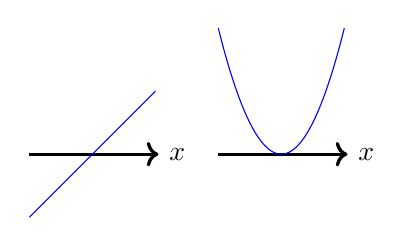
\begin{tikzpicture}[scale=.4][domain=-2:2]
%    \draw[gray!50, thin, step=1] (-10,-5) grid (11,5);
    \draw[very thick,->] (-2,0) -- (2.1,0) node[right] {$x$};
%    \draw[very thick,->] (0,-5) -- (0,5.1) node[above] {$y$};

%    \foreach \x in {-10,...,10} \draw (\x,0.05) -- (\x,-0.05) node[below] {\tiny\x};
%    \foreach \y in {-4,...,4} \draw (-0.05,\y) -- (0.05,\y) node[right] {\tiny\y};


  \draw[scale=1,domain=-2:2,smooth,variable=\x,blue] plot ({\x},{\x});% node[above]{$f(x)$};

    \draw[very thick,->] (4,0) -- (8.1,0) node[right] {$x$};
%    \draw[very thick,->] (0,-5) -- (0,5.1) node[above] {$y$};

%    \foreach \x in {-10,...,10} \draw (\x,0.05) -- (\x,-0.05) node[below] {\tiny\x};
%    \foreach \y in {-4,...,4} \draw (-0.05,\y) -- (0.05,\y) node[right] {\tiny\y};


  \draw[scale=1,domain=4:8,smooth,variable=\x,blue] plot ({\x},{(\x-6)^2});% node[above]{$f(x)$};



\end{tikzpicture}$$ % of mbox

We notice that $p(x)$ only changes sign when it's factors $(x-r_i)^{m_i}$ changes sign.  But $(x-r_i)^{m_i}$ only changes sign if $m_i$ is odd.  So we have the following fact:
\begin{remark}
The polynomial $p(x)$ ``crosses" the $x$-axis at $r_i$ if $m_i$ is odd and ``bounces" if $m_i$ is even.
\end{remark}

\begin{example}
Let $$p(x)=x^3-3x^2=x^2(x-3).$$  \url{https://www.desmos.com/calculator/iy0chaljdq} Since it is a odd degree polynomial with positive leading coefficient, it goes up to $\infty$ as $x$ goes to $\infty$ and down to $-\infty$ as $x$ goes to $-\infty$.  We also see that $p(x)=0$ whenever $x=0$ or $x=3$.  The multiplicity of 0 is 2, and the multiplicity of 3 is 1, which are even and odd respectively, so $p(x)$ ``bounces" at $x=0$ and crosses at $x=1$.

$$  \begin{tikzpicture}[scale=.5]
    \begin{axis}[
        restrict y to domain=-5:5,
        samples=1000,
        minor tick num=1,
        xmin = -3, xmax = 4,
        ymin = -5, ymax = 5,
        unbounded coords=jump,
        axis x line=middle,
        axis y line=middle]

      \addplot[mark=none, domain=-3:4] {\x^3-3*\x^2};
    \end{axis}
  \end{tikzpicture}$$
 % of mbox



\end{example}



\begin{example}
Let $$p(x)=x^4-2x^2+1=(x-1)^2(x+1)^2.$$  \url{https://www.desmos.com/calculator/wmr67oopgj}  Since it is a even degree polynomial with positive leading coefficient, it goes up to $\infty$ as $x$ goes to both positive and negative $\infty$.  We also see that $p(x)=0$ whenever $x=-1$ or $x=1$.  The multiplicity of both of these roots is 2,  so $p(x)$ ``bounces" at both $x=1$ and $x=-1$.

$$  \begin{tikzpicture}[scale=.5]
    \begin{axis}[
        restrict y to domain=-5:5,
        samples=1000,
        minor tick num=1,
        xmin = -3, xmax = 3,
        ymin = -5, ymax = 5,
        unbounded coords=jump,
        axis x line=middle,
        axis y line=middle]

      \addplot[mark=none, domain=-3:3] {\x^4-2*\x^2+1};
    \end{axis}
  \end{tikzpicture}$$
 % of mbox



\end{example}









\section{Rational Functions}\label{Section:RationalFunctions}

\begin{definition}
A \textbf{rational function} is a function $r(x)$ which may be written as $r(x)=\frac{p(x)}{q(x)}$ where $p(x), q(x)$ are both polynomials, and $q(x)\neq 0$.
\end{definition}

Now when we say $q(x)\neq0$, we mean that $q(x)$ is not the polynomial 0, not that $q(x)$ could never be 0.  As before, we will consider the long and short term behavior of polynomials.

\subsection{Long Term Behavior}

For Polynomials, what determined the long term behavior of a polynomial was the leading term.  So it makes sense that a rational function will be determined the same way.  Given  $$r(x)=\frac{a_nx^n+\cdots a_0x^0}{b_mx^m+\cdots b_0x^0},$$ we can determine the long term behavior with $$\frac{a_nx^n}{b_mx^m}$$ which simplifies to $\frac{a_n}{b_m}x^{n-m}$.  So there are some cases to consider here:

\begin{itemize}
\item If $n>m$, then $\frac{a_n}{b_m}x^{n-m}$ is just a regular monomial.  This doesn't mean that $r(x)$'s graph will look like a polynomial's, but it does mean the long term behavior will be the same as that of a polynomial.\\

For example consider $y=\frac{-x^4+x}{x+1}$.  We should note: $\frac{-x^4-x}{x+1}\sim\frac{-x^4}{x}
\sim -x^3$, so the long term behavior of $y$ will be the same as $-x^3$'s:  positive infinity to the left, negative infinity to the right.  \url{https://www.desmos.com/calculator/jzxyyrcgep}.

\item If $n=m$, then $\frac{a_n}{b_m}x^{n-m}=\frac{a_n}{b_m}$ is just a constant.  So as the magnitude of $x$ grows, these values approach $\frac{a_n}{b_m}$.\\

For example consider $y=\frac{-2x^4+x}{3x^4+1}$.  We should note: $\frac{-2x^4-x}{3x^4+1}\sim\frac{-2x^4}{3x^4}
\sim -\frac{2}{3}$, so the long term behavior of $y$ will be the same as $-\frac{2}{3}$'s:   \url{https://www.desmos.com/calculator/qaeq86mivp}.
 
\item If $n<m$, then $\frac{a_n}{b_m}x^{n-m}=\frac{a_n}{b_m}\frac{1}{x^{m-n}}$.  As the magnitude of $x$ grows, the more $\frac{1}{x^{m-n}}$ will shrink and the entire function converges to 0.\\

For example consider $y=\frac{-2x^2+x}{3x^4+1}$.  We should note: $\frac{-2x^2-x}{3x^4+1}\sim\frac{-2x^2}{3x^4}
\sim -\frac{2}{3}\frac{1}{x^2}$, so the long term behavior of $y$ will be converging to 0:   \url{https://www.desmos.com/calculator/n0ftbxmcod}.
 
 
\end{itemize}


\subsection{Short term behavior}

Here, we once again care about the multiplicity of the roots, that is, if $r(x)=\frac{p(x)}{q(x)}$, what we care about is when $p(x)$ or $q(x)$ is 0, and what the multiplicity is.\\

Well, turns out, 0 divided by anything is 0.  So if the numerator is 0, then $r(x)$ is 0.  Moreover, it bounces or crosses in the same way as a polynomial.  So if the multiplicity is odd, the function crosses and if it's even, it bounces.\\

For example, consider $r_1(x)=\frac{x-1}{x}$.  It is clearly 0 when $x=1$, and since the multiplicity is odd, we cross \url{https://www.desmos.com/calculator/9graa40kq1}.  But if we change that to $r_2(x)=\frac{(x-1)^2}{x}$, the multiplicity is now even so we bounce \url{https://www.desmos.com/calculator/iy9kvoac37}.\\

It also turns out you can't divide by 0.  So at those points, the function is undefined.  And as the values in the denominator towards 0, the overall value of the quotient approaches either positive or negative infinity.  Just like roots, whether or not we change signs at these asymptotes depends on the multiplicity of the root.\\




For example, again consider $r_1(x)=\frac{x-1}{x}$.  The denominator is 0 when $x=0$, so we have a vertical asymptote there.  Since the multiplicity is odd, we change signs there: \url{https://www.desmos.com/calculator/ik9xwhui5i}.  If we made that multiplicity even, the function would not change sign at $x=0$, so for $r_2(x)=\frac{x-1}{x^2}$: \url{https://www.desmos.com/calculator/h5famtu30t}






\section{Exponentials}\label{Section:Exponentials}

\begin{definition}
An \textbf{exponential function} is a function $f(x)$ which may be written as $f(x)=b\cdot a^x$.
\end{definition}

We should note that we've seen exponential functions before, in the guise of compound interest.  If the future value of a debt is $S=P(1+i)^x$ after $x$ unites of time, then $P$ is your $b$ and $1+i$ is your $a$.\\

We should also note that there is a real kinship between exponential functions and linear functions.  Linear functions have the form $\ell(x)=mx+b$, which we can think of as $\ell(x)=\overbrace{m+m+\cdots+m}^x+b$, with $x$ copies of $m$.  Similarly we can see that $f(x)=b\cdot a^x=\overbrace{a\cdot a\cdots a}^x\cdot b$, so it is really the multiplicative analogue of the linear function, where the $b$'s are the initial value of the function when $x=0$ and the growth rate of the function is totally determined by $a$ (whereas it's determined by $m$ for linear functions).\\

In that way, we can also tell when $f(x)=b\cdot a^x$ is increasing or decreasing, just by looking at whether or not $a>1$ or $a<1$.  If $a>1$ it is increasing: \url{https://www.desmos.com/calculator/edktzphc6x} if $a<1$ then it's decreasing: \url{https://www.desmos.com/calculator/rpiu9qc4ty}.\\


Exponential functions are used to model anything that grows or decays proportionately to  it's current value.  So for example debts or investment accrue proportionately to how much debt/investment there already is.  Population is another example, the greater the population, the more reproduction there will be within that population and the greater the increase in population.

\section{Logarithms}\label{Section:Logarithms}

So looking at any exponential function, but specifically for increasing ones, we notice that they are 1-1, meaning two different inputs give you 2 different outputs.  Thus, $f(x)=a^x$ is an invertible function.  You can see in these graphs \url{https://www.desmos.com/calculator/cvriy608bg} that reflecting the exponential over the $y=x$ line giving us the green function is another function.  We call this function $\log_a(x)$.  As the inverse of an exponential function, it has some properties:

\begin{itemize}
\item \textbf{It's domain is only positive numbers}.  Why?  Because the only possible outputs of exponential outputs are positive numbers.  Taking the inverse reverses the roles of the domain and range, and so the domain of $\log_a$ is the positives.
\item \textbf{As $\mathbf{x}$ goes to 0, $ \mathbf{\log_a(x)}$ goes to $\mathbf{-\infty}$.}   This is the result of the reflection.  Normally $a^x$ (for $a>1$) goes to 0 as $x\to -\infty$, so when reflected, that line is now asymptotic to the $y$-axis.  Also $\log_a$ returns the power necessary to achieve the value $x$.  If $x$ is a small number like 0.0001, what power would I have to raise $a$ to to get $0.0001$?  It can't be 0, $a^0=1$, so it has to be \textbf{less} than 0, and the smaller $x$ is, the lower this power must go.

\item  As $\mathbf{x\to\infty, \log_a(x)\to \infty}$, again this is the result  of the reflection, but we can also think of this as the powers $a$ needs to be raised to in order to achieve $x$, as this increases, those powers must increase as well.

\item $\log_a(xy)=\log_a(x)+\log_a(y)$. Too see this consider:

\begin{eqnarray*}
xy&=&a^{\log_a{xy}}\\
xy&=&x\cdot y\\
&=&a^{\log_a(x)}\cdot a^{\log_a(y)}\\
&=&a^{\log_a(x)+\log_a(y)}.
\end{eqnarray*}


\item $\log_a(x^y)=y\log_a(x)$.  To see this, consider:

\begin{eqnarray*}
x^y&=&a^{\log_a(x^y)}.\\
x^y&=&(a^{\log_a(x)})^y\\
&=&a^{y\log_a(x)}
\end{eqnarray*}



\end{itemize}

Typically most textbooks include a whole bunch of other arithmetic rules, but they can all be distilled from the 2 above so they're all totally pointless.\\

Special cases of logs are log base 10 which is usually just denoted $\log$ and log based $e$, which is denoted $\ln$.  Astronomers and other scientists like $\log$ since taking $\log$ base 10 gives you approximate magnitude of stuff.  As a mathematician, I prefer $\ln$ since $e$ has pretty special mathematical properties, plus it's shorter, which makes it better.\\

The main use of logs algebraically is to de-exponentiate expressions.  So if one is trying to solve $10=2^x$, we could do this via:

\begin{eqnarray*}
10&=&2^x\\
\ln(10)&=&\ln(2^x)\\
\ln(10)&=&x\ln(2)\\
x&=&\frac{\ln(10)}{\ln(2)}\approx 3.3219.
\end{eqnarray*}

One can also solve problems like this visually:  \url{https://www.desmos.com/calculator/t0pojr0gel}.














\chapter{Introduction to Differential Calculus}\label{Chapter:Calculus}


\section{Limits \& Continuity}\label{Section:LimitsContinuity}

Informally, the limit of a function $\limit{x}{a} f(x)=L$ (if it exists) is a number $L$ such that when $f(x)$ get's closer and closer to $a$, $f(x)$ gets closer and closer to $L$. \\

Consider the function $f(x)=\frac{x^2-1}{x-1}$, what happens as $x$ get's closer and closer to 1?

$$
\begin{array}{|c|c|}
\hline
x & f(x)\\
\hline
1.1 & 2.1\\
1.01 & 2.01\\
1.001 & 2.001\\
.9 & 1.9\\
.99&1.99\\
.999 & 1.999\\
\hline
\end{array}$$

You can test and see these values here: \url{https://www.desmos.com/calculator/w3ycpf3mv4}.  It certainly seems as if $x$ gets closer and closer to $1$, $f(x)$ approaches the value $2$.  Why couldn't we just plug in 1?  Because if we did we would get $f(1)``="\frac{1^2-1}{1-1}``="\frac{0}{0}$ which is undefined.  Recall that $1$ would not be a part of the domain of $f(x)$.  This, in fact, is the whole point of limits, the entire reason they exist, is in order to give values to things like $f(1)$ which are not defined.\\

The left and right limits of a function are values the function approaches as $x$ $a$ from the left or the right, so as we see above, they both (the black and orange dots in the linked graph) both approach the same value.  So:

\begin{itemize}
\item $\limit{x}{1^-}\frac{x^2-1}{x-1}=2$.
\item $\limit{x}{1^+}\frac{x^2-1}{x-1}=2$
\item $\limit{x}{1}\frac{x^2-1}{x-1}=2$
\item $f(1)$ is undefined.
\end{itemize}

So looking at this graph:
$$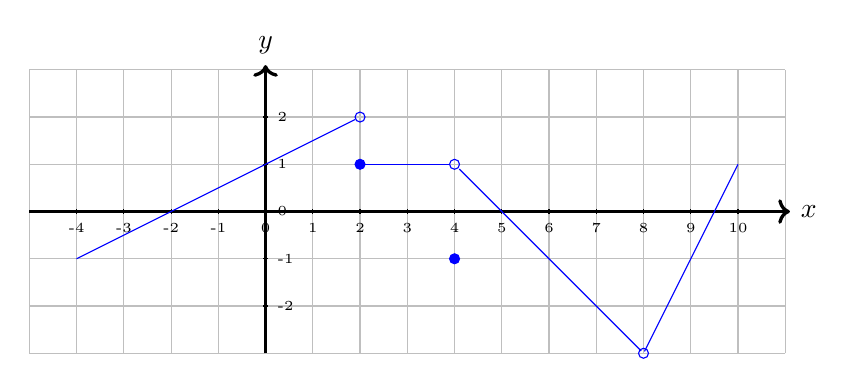
\begin{tikzpicture}[scale=.6][domain=-5:11]
    \draw[gray!50, thin, step=1] (-5,-3) grid (11,3);
    \draw[very thick,->] (-5,0) -- (11.1,0) node[right] {$x$};
    \draw[very thick,->] (0,-3) -- (0,3.1) node[above] {$y$};

    \foreach \x in {-4,...,10} \draw (\x,0.05) -- (\x,-0.05) node[below] {\tiny\x};
    \foreach \y in {-2,...,2} \draw (-0.05,\y) -- (0.05,\y) node[right] {\tiny\y};

    \draw[blue] (2,2) circle (3pt);
    \draw[ blue, fill] (2,1) circle (3pt);
    \draw[blue] (4,1) circle (3pt);
    \draw[fill, blue] (4,-1) circle (3pt);
    \draw[blue] (8,-3) circle (3pt);


  \draw[scale=1,domain=-4:1.9,smooth,variable=\x,blue] plot ({\x},{.5*\x+1});
  \draw[scale=1,domain=2.1:3.9,smooth,variable=\x,blue] plot ({\x},{1});
  \draw[scale=1,domain=4.1:7.95,smooth,variable=\x,blue] plot ({\x},{-1*\x+5});
  \draw[scale=1,domain=8.02:10,smooth,variable=\x,blue] plot ({\x},{2*\x-19});


\end{tikzpicture}$$

For $x=2,4,6,8$, find the left and right limits, the limit, and the value of the function.  See if you understand why the following are true:

\begin{itemize}
\item $\limit{x}{2^-}f(x)=2$, as we approach $x$ from the left, this is what $f(x)$ approaches.
\item $\limit{x}{2^+}f(x)=1$, as we approach $x$ from the right, this is what $f(x)$ approaches.
\item $\limit{x}{2}f(x)$ is undefined, there is no single number that $f(x)$ get's closer to, so there is no limit.
\item $f(2)=1$, that's the actual value of $f(2)$.
\end{itemize}

Similarly, we should see:

\begin{itemize}
\item $\limit{x}{4^-}f(x)=1$.
\item $\limit{x}{4^+}f(x)=1$.
\item $\limit{x}{4}f(x)=1$.
\item $f(4)=-1$.
\item $\limit{x}{6^-}f(x)=-1$.
\item $\limit{x}{6^+}f(x)=-1$.
\item $\limit{x}{6}f(x)=-1$.
\item $f(6)=-1$.
\item $\limit{x}{8^-}f(x)=-3$.
\item $\limit{x}{8^+}f(x)=-3$.
\item $\limit{x}{8}f(x)=-3$.
\item $f(8)$ is undefined.
\end{itemize}

A great shorthand for determining when there is or isn't a limit is: ``$\limit{x}{a}f(x)=L$ and exists if and only if $\limit{x}{a^-}f(x)=L$ and $\limit{x}{a^+}f(x)=L$"

\subsection{Continuity}

I'm not going to overblow continuity with to much verbiage here since we intuitive understand what it means to be continuous, it just means that all the points ``connect".  So what does tat mean for us above?  Out of the values $x=2,4,6,8$, where is $x$ continuous?

It seems like it's only 6 where it's continuous.  2 and 4 have jump discontinuities, and $f(x)$ isn't even defined at $x=8$ so how could it be continuous there?  So the definition of continuous is as intuitive as we would like:\\

$f(x)$ is continuous at $a$ if and only of $f(a)=\limit{x}{a} f(x)$.  So as in above, out of the 4 points we looked at, $x=6$ is the only place where everything ``behaves properly" and we get continuity.




\section{Average rates of change}\label{Section:AvgRoC}

Consider a rocket that is launched into the air and has height $f(x)=-5x^2+20x$ meters in $x$ seconds. \url{https://www.desmos.com/calculator/1rwsdsbcm9}. How fast is the rocket traveling when it's launched ($x=0$ seconds)?\\

Turns out, it's not so easy to think about what this is, we don't typically think about speeds in terms of instantaneous action.  Our methods of measuring speed reflects this, it's always stuff like meters \textbf{ PER SECOND}, miles \textbf{ PER HOUR}, in other words speed is some change in distance \textbf{ OVER TIME} and that period of time is not typically 0.\\

So what now?  Lets start by asking an easier question, what is the average speed of the rocket over the first 3 seconds?\\

It's best in a scenario like this to NOT overthink the underlying problem.  At 0 seconds, you're $f(0)=-5(0)^2+20(0)=0$ meters off the ground.  After 3 seconds you are $f(3)=-5(3^2)+20(3)=15$ meters off the ground.  So you rose by 15 meters in 3 seconds?  You're aveerage speed must be 5 meters per second. \url{https://www.desmos.com/calculator/6k61owwnrd}.\\

In fact:  \textbf{ The average rate of change of a function $f(x)$ over the interval $[a,b]$ is $m=\frac{f(b)-f(a)}{b-a}$.}  This is just the slope of the line connecting $(a,f(a))$ and $(b,f(b))$.\\

Following this idea, the average velocity of our rocket over the 1st 2 seconds is: $m=\frac{f(2)-f(0)}{2-0}=\frac{20}{2}=10$ meters per second. \url{https://www.desmos.com/calculator/ihauynuflo}\\

The average velocity of our rocket over the 1st second is: $m=\frac{f(1)-f(0)}{1-0}=\frac{15}{1}=15$ meters per second. \url{https://www.desmos.com/calculator/jce0fd1bsr}\\

The average velocity of our rocket over the 1st half second is: $m=\frac{f(.5)-f(0)}{.5-0}=\frac{8.75}{.5}=17.5$ meters per second. \url{https://www.desmos.com/calculator/xpxlltf8f5}\\

The average velocity of our rocket over the 1st quarter second is: $m=\frac{f(.25)-f(0)}{.25-0}=\frac{4.6875}{.25}=18.75$ meters per second. \url{https://www.desmos.com/calculator/74kpvz17c5}\\

The average velocity of our rocket over the 1st tenth of a second is: $m=\frac{f(.1)-f(0)}{.1-0}=\frac{1.95}{.1}=19.5$ meters per second. \url{https://www.desmos.com/calculator/qyvtzmyg8k}\\

The average velocity of our rocket over the 1st hundreth of a second is: $m=\frac{f(.01)-f(0)}{.01-0}=\frac{.1995}{.1}=19.95$ meters per second. \url{https://www.desmos.com/calculator/hrawtifwdw}\\


And it does seem like these numbers are getting closer and closer to 20 meters per second as $b$ gets closer to 0.  But if I plug in $0$ for $b$, I get an undefined $0/0$ fraction.  Oh, if only there were some concept in mathematics to describe the values of a function as your inputs slowly approach a given value.........

\section{The Derivative as a Limit}\label{Section:DefofDerivative}

Let's be a bit more general for just a moment, suppose that we had a function $f(x)$ and we wanted to know what the instantaneous rate of change of a function was at some given $x$.  Well, if we stepped forward by $h$ units, we could measure the average rate of change of $f(x)$ over $[x, x+h]$, this would be $$\frac{f(x+h)-f(x)}{x+h-x}=\frac{f(x+h)-f(x)}{h}.$$

What we just observed is that if we let $h$ converge towards 0, that it seems as if our quotient also converges to some value.  This value is the derivative of $f(x)$ at $x$ and is denoted and defined as $$f'(x)=\limit{h}{0}\frac{f(x+h)-f(x)}{h}.$$

So how does this play out given our rocket?  Well:

\begin{eqnarray*}
f'(x)&=&\limit{h}{0}\frac{f(x+h)-f(x)}{h}\\
&=&\limit{h}{0} \frac{-5(x+h)^2+20(x+h)-(-5x^2+20x)}{h}\\
&=&\limit{h}{0}\frac{-5x^2-10xh-5h^2+20x+20h+5x^2-20x}{h}\\
&=&\limit{h}{0}\frac{-10xh-5h^2+20h}{h}\\
&=&\limit{h}{0}\frac{(-10x-5h+20)h}{h}\\
&=&\limit{h}{0} -10x-5h+20\\
&=&-10x+20.
\end{eqnarray*}


So this means that in $0$ seconds, the change in the height was $f'(0)=-10(0)+20=20$ meters/second as we suspected!  But now we can compute all the other instantaneous rates of change as well.  So at $t=1$ second, it'll be $f'(1)=-10(1)+20=10$ meters per second.  In 2 seconds we are at the top with $f'(2)=0$ meters per second, at 3 seconds, $f'(3)=-10$ meters/second to reflect the negative change in height at this point.  Finally in 4 seconds, the rocket hits the ground at $f'(4)=-20$ meters per second.  (drag $a$ around and see for yourself! \url{https://www.desmos.com/calculator/3po0qezgel})




\section{Basic rules of the derivative}\label{Section:RulesofDerivative}

At this point we probably are, or should be, sick of computing limits like: $$\limit{h}{0}\frac{2(x+h)^3-4(x+h)-(2x^3-4x)}{h}.$$  This is technically the derivative of $f(x)=2x^3-4x$.  But there's 2 sides to mathematics, theres the formal definition, and then we should leverage our knowledge and try to find shortcuts to some of these things.  So let's  figure some of these things out.\\

Given functions $f(x), g(x)$ and constants $a,b$ we have: $$\frac{d}{dx}[a(f)x)+bg(x)]=af'(x)+bg'(x).$$  How do we know that?  Well:

\begin{eqnarray*}
\frac{d}{dx}[a(f)x)+bg(x)]&=&\limit{h}{0}\frac{af(x+h)+bg(x+h)-(af(x)-bg(x))}{h}\\
&=&\limit{h}{0}\frac{af(x+h)-af(x)}{h}+\limit{h}{0}\frac{bg(x+h)-bg(x)}{h}\\
&=&a\limit{h}{0}\frac{f(x+h)-f(x)}{h}+b\limit{h}{0}\frac{g(x+h)-g(x)}{h}\\
&=&af'(x)+bg'(x).
\end{eqnarray*}

\section{Power Rule}\label{Section:PowerRule}

We may have noticed a pattern with derivatives.  But to illustrate it explicitly:

\begin{itemize}
\item The derivative of $f(x)=x^0$, it's the derivative of the  constant function $f(x)=1$, and since its a horizontal line, it never has any slope and $f'(x)=0$.
\item  The derivative of $f(x)=x^1$, it's the derivative of the line $f(x)=x$ which always has slope 1, so $f'(x)=1$.

\item The derivative of $f(x)=x^2$ is:

\begin{eqnarray*}
f(x)&=&\limit{h}{0}\frac{f(x+h)-f(x)}{h}\\
&=&\limit{h}{0} \frac{(x+h)^2-x^2}{h}\\
&=&\limit{h}{0} \frac{x^2+2xh+h^2-x^2}{h}\\
&=&\limit{h}{0} \frac{(2x+h)h}{h}\\
&=&\limit{h}{0} 2x+h=2x.\\
\end{eqnarray*}


\item The derivative of $f(x)=x^3$ is:

\begin{eqnarray*}
f(x)&=&\limit{h}{0}\frac{f(x+h)-f(x)}{h}\\
&=&\limit{h}{0} \frac{(x+h)^3-x^3}{h}\\
&=&\limit{h}{0} \frac{x^3+3x^2h+3xh^2+h^3-x^3}{h}\\
&=&\limit{h}{0} \frac{(3x^2+3xh+h^2)h}{h}\\
&=&\limit{h}{0} 3x^2+3xh+h^2=3x^2.\\
\end{eqnarray*}
 
\end{itemize}

To generalize this, we have a rule of differentiation called the \textbf{ power rule} which goes: $\frac{d}{dx}[x^n]=nx^{n-1}$. \\ 

To verify:

\begin{itemize}
\item $\frac{d}{dx}[x^0]=0x^{0-1}=0$.
\item $\frac{d}{dx}[x^1]=1x^{1-1}=1$.
\item $\frac{d}{dx}[x^2]=2x^{2-1}=2x$.
\item $\frac{d}{dx}[x^3]=3x^{3-1}=3x^2$.
\end{itemize}

What's fascinating is that this rule applies to \textbf{ all} powers, not just integer powers.


\subsection{Examples}

We can combine these rules to find the derivatives of some basic functions.  So consider the derivative of $f(x)=x^4-2x^2+7x-3$.  It would be:

\begin{eqnarray*}
f'(x)&=&\frac{d}{dx}[x^4-2x^2+7x-3]\\
&=&\frac{d}{dx}[x^4-2x^2+7x^1-3x^0]\\
&=&4x^3-2(2x^1)+7(1x^0)-3(0x^{-1})\\
&=&12x^3-4x+7.
\end{eqnarray*}

Whereas the derivative of $g(x)=\sqrt{4x}+\frac{3}{x}-\frac{2}{x^2}$ would be:

\begin{eqnarray*}
g'(x)&=&\frac{d}{dx}[\sqrt{4x}+\frac{3}{x}-\frac{2}{x^2}]\\
&=&\frac{d}{dx}[2x^{1/2}+3x^{-1}-2x^{-2}]\\
&=&2(1/2)x^{-1/2}+3(-1x^{-2})-2(2x^{-3})\\
&=&x^{-1/2}-3x^{-2}+4x^{-3}\\
&=&\frac{1}{\sqrt{x}}-\frac{3}{x^2}+\frac{4}{x^3}.
\end{eqnarray*}



\section{Product Rule}\label{Section:ProductRule}

Since the behavior of derivatives of sums behave so well, its tempting to believe that the derivatives of products would behave similarly well, that is, it may be reasonable to guess that $\frac{d}{dx}[f(x)g(x)]=f'(x)g'(x)$.  To try to see if this is true, we should ask, is:

$$\frac{d}{dx}[x\cdot x]=\frac{d}{dx}[x]\frac{d}{dx}[x]?$$

Well on the left hand side $\frac{d}{dx}[x\cdot x]=\frac{d}{dx}[x^2]=2x$.  On the right, $\frac{d}{dx}[x]\frac{d}{dx}[x]=1\cdot1=1$, so these are clearly not the same.  What should it be?\\

We do have a rule for products called the \textbf{ product rule} and it states $\frac{d}{dx}[f(x)g(x)]=f'(x)g(x)+f(x)g'(x).$  To see why:

\begin{eqnarray*}
\frac{d}{dx}[f(x)g(x)]&=&\limit{h}{0}\frac{f(x+h)g(x+h)-f(x)g(x)}{h},\ \text{at this stage, I'm going to pull a clever trick and add by 0:}\\
&=&\limit{h}{0}\frac{f(x+h)g(x+h)\textcolor{blue}{-f(x)g(x+h)+f(x)g(x+h)}-f(x)g(x)}{h}\\
&=&\limit{h}{0}\frac{f(x+h)g(x+h)-f(x)g(x+h)}{h}+\limit{h}{0}\frac{f(x)g(x+h)-f(x)g(x)}{h}\\
&=&\limit{h}{0}\frac{f(x+h)-f(x)}{h}g(x+h)+\limit{h}{0}f(x)\frac{g(x+h)-g(x)}{h}\\
&=&f'(x)g(x)+f(x)g'(x).
\end{eqnarray*}



\section{Quotient Rule}\label{Section:QuotientRule}

If we have a rule for differentiating products, we should have a rule for differentiating quotients as well, after all, quotients and products are basically the same thing.  So let $Q(x)=\frac{f(x)}{g(x)}$, and ask, what is $Q'(x)$.  So:

\begin{eqnarray*}
Q(x)&=&\frac{f(x)}{g(x)}\\
Q(x)g(x)&=&f(x),\ \text{now we can differentiate both sides}\\
\frac{d}{dx}[Q(x)g(x)]&=&f'(x),\ \text{then by the product rule:}\\
Q'(x)g(x)+Q(x)g'(x)&=&f'(x)\\
Q'(x)g(x)&=&f'(x)-Q(x)g'(x),\ \text{then recall that  $Q(x)=\frac{f(x)}{g(x)}$}\\
Q'(x)g(x)&=&f'(x)-\frac{f(x)g'(x)}{g(x)}\\
Q'(x)g(x)&=&\frac{f'(x)g(x)-f(x)g'(x)}{g(x)}\\
Q'(x)&=&\frac{f'(x)g(x)-f(x)g'(x)}{g(x)^2}\\
\end{eqnarray*}


So the \textbf{ quotient rule} is $\frac{d}{dx}[\frac{f(x)}{g(x)}]=\frac{f'(x)g(x)-f(x)g'(x)}{g(x)^2}$.


\subsection{Examples}

So, consider the derivative of $f(x)=x^3(x+1)$, which can be computed:

\begin{eqnarray*}
f'(x)&=&\frac{d}{dx}[x^3](x+1)+x^3\frac{d}{dx}[x+1]\\
&=&3x^2(x+1)+x^3(1)\\
&=&3x^3+3x^2+x^3\\
&=&4x^3+3x^2.
\end{eqnarray*}

Also note we could have computed this some other way:

\begin{eqnarray*}
f(x)&=&x^3(x+1)=x^4+x^3\\
f'(x)&=&4x^3+3x^2.
\end{eqnarray*}

Similarly, the derivative of $g(x)=\frac{x}{x^2+1}$:

\begin{eqnarray*}
g'(x)&=&\frac{(x^2+1)\frac{d}{dx}[x]-x\frac{d}{dx}[x^2+1]}{(x^2+1)^2}\\
&=&\frac{(x^2+1)(1)-x(2x)}{(x^2+1)^2}\\
&=&\frac{1-x^2}{(x^2+1)^2}\\
\end{eqnarray*}




\section{Product Rule}

Since the behavior of derivatives of sums behave so well, its tempting to believe that the derivatives of products would behave similarly well, that is, it may be reasonable to guess that $\frac{d}{dx}[f(x)g(x)]=f'(x)g'(x)$.  To try to see if this is true, we should ask, is:

$$\frac{d}{dx}[x\cdot x]=\frac{d}{dx}[x]\frac{d}{dx}[x]?$$

Well on the left hand side $\frac{d}{dx}[x\cdot x]=\frac{d}{dx}[x^2]=2x$.  On the right, $\frac{d}{dx}[x]\frac{d}{dx}[x]=1\cdot1=1$, so these are clearly not the same.  What should it be?\\

We do have a rule for products called the \textbf{ product rule} and it states $\frac{d}{dx}[f(x)g(x)]=f'(x)g(x)+f(x)g'(x).$  To see why:

\begin{eqnarray*}
\frac{d}{dx}[f(x)g(x)]&=&\limit{h}{0}\frac{f(x+h)g(x+h)-f(x)g(x)}{h},\ \text{at this stage, I'm going to pull a clever trick and add by 0:}\\
&=&\limit{h}{0}\frac{f(x+h)g(x+h)\textcolor{blue}{-f(x)g(x+h)+f(x)g(x+h)}-f(x)g(x)}{h}\\
&=&\limit{h}{0}\frac{f(x+h)g(x+h)-f(x)g(x+h)}{h}+\limit{h}{0}\frac{f(x)g(x+h)-f(x)g(x)}{h}\\
&=&\limit{h}{0}\frac{f(x+h)-f(x)}{h}g(x+h)+\limit{h}{0}f(x)\frac{g(x+h)-g(x)}{h}\\
&=&f'(x)g(x)+f(x)g'(x).
\end{eqnarray*}



\section{Quotient Rule}

If we have a rule for differentiating products, we should have a rule for differentiating quotients as well, after all, quotients and products are basically the same thing.  So let $Q(x)=\frac{f(x)}{g(x)}$, and ask, what is $Q'(x)$.  So:

\begin{eqnarray*}
Q(x)&=&\frac{f(x)}{g(x)}\\
Q(x)g(x)&=&f(x),\ \text{now we can differentiate both sides}\\
\frac{d}{dx}[Q(x)g(x)]&=&f'(x),\ \text{then by the product rule:}\\
Q'(x)g(x)+Q(x)g'(x)&=&f'(x)\\
Q'(x)g(x)&=&f'(x)-Q(x)g'(x),\ \text{then recall that  $Q(x)=\frac{f(x)}{g(x)}$}\\
Q'(x)g(x)&=&f'(x)-\frac{f(x)g'(x)}{g(x)}\\
Q'(x)g(x)&=&\frac{f'(x)g(x)-f(x)g'(x)}{g(x)}\\
Q'(x)&=&\frac{f'(x)g(x)-f(x)g'(x)}{g(x)^2}\\
\end{eqnarray*}


So the \textbf{ quotient rule} is $\frac{d}{dx}[\frac{f(x)}{g(x)}]=\frac{f'(x)g(x)-f(x)g'(x)}{g(x)^2}$.


\subsection{Examples}

So, consider the derivative of $f(x)=x^3(x+1)$, which can be computed:

\begin{eqnarray*}
f'(x)&=&\frac{d}{dx}[x^3](x+1)+x^3\frac{d}{dx}[x+1]\\
&=&3x^2(x+1)+x^3(1)\\
&=&3x^3+3x^2+x^3\\
&=&4x^3+3x^2.
\end{eqnarray*}

Also note we could have computed this some other way:

\begin{eqnarray*}
f(x)&=&x^3(x+1)=x^4+x^3\\
f'(x)&=&4x^3+3x^2.
\end{eqnarray*}

Similarly, the derivative of $g(x)=\frac{x}{x^2+1}$:

\begin{eqnarray*}
g'(x)&=&\frac{(x^2+1)\frac{d}{dx}[x]-x\frac{d}{dx}[x^2+1]}{(x^2+1)^2}\\
&=&\frac{(x^2+1)(1)-x(2x)}{(x^2+1)^2}\\
&=&\frac{1-x^2}{(x^2+1)^2}\\
\end{eqnarray*}


\section{Chain Rule}\label{Section:ChainRule}

We've so far covered sums products and quotients of functions, so how about composition?   The \textbf{ chain rule} is: $\frac{d}{dx}[f(g(x))]=f'(g(x))g'(x)$.  To see why:

\begin{eqnarray*}
\frac{d}{dx}[f(g(x))]&=&\limit{h}{0}\frac{f(g(x+h))-f(g(x))}{h},\ \text{Similar to the product rule, we will multiply by 1:}\\
&=&\limit{h}{0}\frac{f(g(x+h))-f(g(x))}{h}\textcolor{blue}{\frac{g(x+h)-g(x)}{g(x+h)-g(x)}}\\
&=&\limit{h}{0}\frac{f(g(x+h))-f(g(x))}{g(x+h)-g(x)}\frac{g(x+h)-g(x)}{h}\\
&=&\limit{h}{0}\frac{f(g(x+h))-f(g(x))}{g(x+h)-g(x)}\limit{h}{0}\frac{g(x+h)-g(x)}{h}\\
\end{eqnarray*}

We're going tom play a second trick here, we are goin to let $k=g(x+h)-g(x)$, we also note then that $g(x+h+=g(x)+k$.  Also note that when $h\to 0$  It follows that $k=g(x+h)-g(x)\to g(x+0)-g(x)=0$.  So we can make some replacements:

\begin{eqnarray*}
&=&\limit{h}{0}\frac{f(g(x+h))-f(g(x))}{g(x+h)-g(x)}\limit{h}{0}\frac{g(x+h)-g(x)}{h}\\
&=&\limit{\textcolor{red}{k}}{0}\frac{f(\textcolor{red}{g(x)+k})-f(g(x))}{\textcolor{red}{k}}\limit{h}{0}\frac{g(x+h)-g(x)}{h}\\
&=&f'(g(x))g'(x)
\end{eqnarray*}

\subsection{Examples}

Consider $f(x)=\sqrt{x^2+1}$.  We can think of this as $f(x)=g(h(x))$ where $g(x)=\sqrt{x}=x^{1/2}, h(x)=x^2+1$.  So $g'(x)=\frac{1}{2}x^{-1/2}, h'(x)=2x$ and:

\begin{eqnarray*}
f'(x)&=&\frac{d}{dx}[\sqrt{x^2+1}]\\
&=&\frac{d}{dx}[g(h(x))]\\
&=&g'(h(x))h'(x)\\
&=&\frac{1}{2}(x^2+1)^{-1/2}(2x)\\
&=&\frac{x}{\sqrt{x^2+1}}.
\end{eqnarray*}


Another example, lets consider the derivative of $y=(x^2+100)^{300}$.  We COULD expand this polynomial out, but lets agree no one wants that.  On the other hand by the chain rule:

\begin{eqnarray*}
\frac{dy}{dx}&=&\frac{d}{dx}[(x^2+100)^{300}],\ \text{so by the chain rule:}\\
&=&300(x^2+100)^{299}\frac{d}{dx}[x^2+100]\\
&=&300(x^2+100)^{299}(2x)\\
&=&600x(x^2+100)^{299}.
\end{eqnarray*}



\section{Derivative of Exponentials}\label{DerivativeExp}

When we graph an exponential function, say an increasing one $f(x)=a^x, a>1$, we imagine a function that curves up towards infinity on the right and shallows out towards 0 on the left \url{https://www.desmos.com/calculator/51zxitu9xc}.  What then should it's derivatives look like?  Well it seems like the slopes are initially shallow, and then as we go forward the slopes start to increase, and they get progressively and progressively larger.  In other words \textbf{ the derivative is also an exponential function!} \url{https://www.desmos.com/calculator/etbmc1ttzo}.\\

Which one?  Let's first start with a special case, what is the derivative of $f(x)=e^x$?  $e$ is a special number, it has the peculiar property that:

$$\limit{h}{0}\frac{e^h-1}{h}=1.$$  The proof of this is a fairly sophisticated fact and it not trivial, but you can verify it by taking the slider $h$, dragging it towards 0 and seeing what happens: \url{https://www.desmos.com/calculator/4uv0zgguq9}.  Using this fact, we can deduce:

\begin{eqnarray*}
\frac{d}{dx}[e^x]&=&\limit{h}{0}\frac{e^{x+h}-e^x}{h}\\
&=&\limit{h}{0}\frac{e^xe^h-e^x}{h}\\
&=&e^x\limit{h}{0}\frac{e^h-1}{h}\\
&=&e^x\cdot1=e^x.
\end{eqnarray*}


So this explains why $e$ is such a significant number in mathematics, it is the unique number so that the exponential $e^x$ is it's own derivative \url{https://www.desmos.com/calculator/xelrg6t0ez}.   Every other $a^x$ differs from it's derivative slightly: \url{https://www.desmos.com/calculator/aqa6zw4vyz}, you can see that when $a$ is less than $e$ (about 2.714), it's derivative falls under the original function, and when $a>e$, it's derivative falls above the original.\\

So, to compute the actual derivative of $a^x$:

\begin{eqnarray*}
\frac{d}{dx}[a^x]&=&\frac{d}{dx}[(e^{\ln(a)})^x],\ \text{since exponentiating by $e$ and $\ln$ are inverses}\\
&=&\frac{d}{dx}[e^{\ln(a)x}]\\
&=&e^{\ln(a)x}\frac{d}{dx}[\ln(a)x],\ \text{by chain rule}\\
&=&e^{\ln(a)x}\ln(a)\cdot1\\
&=&a^x\ln(a).
\end{eqnarray*}


\section{Logarithms}\label{DerivativeLogs}

We can use the chain rule to find the derivative of log functions as well.  Let's first compute $\frac{d}{dx}[\ln(x)]$:

\begin{eqnarray*}
x&=&e^{\ln(x)}\\
\frac{d}{dx}[x]&=&\frac{d}{dx}[e^{\ln(x)}]\\
1&=&e^{\ln(x)}\frac{d}{dx}[\ln(x)]\\
1&=&x\frac{d}{dx}[\ln(x)]\\
\frac{d}{dx}[\ln(x)]&=&\frac{1}{x}.
\end{eqnarray*}

You can see it graphically verified here: \url{https://www.desmos.com/calculator/u89fjxup7q}.  For general $\log_a(x)$:


\begin{eqnarray*}
x&=&a^{\log_a(x)}\\
\frac{d}{dx}[x]&=&\frac{d}{dx}[a^{\log_a(x)}]\\
1&=&a^{\log_a(x)}\ln(a)\frac{d}{dx}[\log_a(x)]\\
1&=&x\ln(a)\frac{d}{dx}[\log_a(x)]\\
\frac{d}{dx}[\log_a(x)]&=&\frac{1}{x\ln(a)}.
\end{eqnarray*}


Verified graphically here as well: \url{https://www.desmos.com/calculator/znr3xikwcc}.  Drag $a$ around and see how everything matches up.

\subsection{Examples}


Let's try the derivative of $f(x)=e^{x}x^2$:

\begin{eqnarray*}
f'(x)&=&\frac{d}{dx}[e^xx^2]\\
&=_{PR}&\frac{d}{dx}[e^x]x^2+e^x\frac{d}{dx}[x^2]\\
&=&e^xx^2+e^x2x.
\end{eqnarray*}

Let $g(x)=\ln(x^2+1)$:

\begin{eqnarray*}
g'(x)&=&\frac{d}{dx}[\ln(x^2+1)]\\
&=_{CR}&\frac{1}{x^2+1}\frac{d}{dx}[x^2+1]\\
&=&\frac{2x}{x^2+1}.
\end{eqnarray*}

One last one, let $h(x)=2^{\frac{x}{x+1}}$\\

\begin{eqnarray*}
h'(x)&=&\frac{d}{dx}[2^{\frac{x}{x+1}}]\\
&=_{CR}&2^{\frac{x}{x+1}}\ln(2)\frac{d}{dx}[\frac{x}{x+1}]\\
&=_{QR}&2^{\frac{x}{x+1}}\ln(2)\frac{(x+1)\frac{d}{dx}[x]-x\frac{d}{dx}[x+1]}{(x+1)^2}\\
&=&\frac{2^{\frac{x}{x+1}}\ln(2)}{(x+1)^2}
\end{eqnarray*}































\end{document}
